%
% File    : 3yp_report.tex
% Author  : Suleiman Mahmood, Victor Moreno, Eesh Mishra, Rahul Marchand
% Created : 2025
% ____________________________________________________________________________
%
% DESCRIPTION :
%
% Third-year Engineering Group Project Report
% Smartphone-Based mTBI Screening Tool Using Pupillometry
% ____________________________________________________________________________


\documentclass[report,11pt,review,leftmargin=20mm,rightmargin=20mm,topmargin=20mm,bottommargin=20mm]{oxengthesis}


%
% Bibliography: natbib in numerical mode preserves the existing \cite{} → [N]
% behaviour while enabling \citet{key} → "Author et al. [N]" textual citations
% used in chap 9 (business plan) and chap 11 (financial plan).
%https://www.overleaf.com/user/settings#references
\usepackage[numbers]{natbib}
\usepackage{wrapfig}

% Pugh-matrix Harvey-ball symbology (Figure~\ref{fig:pugh-matrix}, \S3.1.2).
% xcolor with [table] option already loaded by oxengthesis.cls; tikz and
% booktabs are added here. Both are idempotent if loaded elsewhere.
\usepackage{tikz}
\usepackage{booktabs}
\definecolor{pughmeets}{RGB}{43,143,72}
\definecolor{pughpartial}{RGB}{216,164,40}
\definecolor{pughnomeet}{RGB}{210,140,140}
\definecolor{pughproprow}{RGB}{223,242,228}
\definecolor{pughheader}{RGB}{47,77,131}
\newcommand{\hbfull}{\tikz[baseline=-0.6ex]{\fill[pughmeets] (0,0) circle (0.22cm);}}
\newcommand{\hbhalf}{\tikz[baseline=-0.6ex]{%
  \draw[pughpartial,line width=1pt] (0,0) circle (0.22cm);%
  \fill[pughpartial] (0,-0.22) arc[start angle=-90,end angle=90,radius=0.22cm] -- cycle;}}
\newcommand{\hbnone}{\tikz[baseline=-0.6ex]{\draw[pughnomeet,line width=1.4pt] (0,0) circle (0.22cm);}}


%
% Global table tightening: mild row-height and column-gap compression applied
% to every table. Values stay above the threshold where readability degrades.
%
\renewcommand{\arraystretch}{0.95}
\setlength{\tabcolsep}{5pt}


%
% Document metadata
%


\title       {Headset-based Oculomotor Screening for mTBI}
\author      {Suleiman Mahmood, Victor Moreno, Eesh Mishra, Rahul Marchand \\ \textit{(Equal contribution)}}
\degree      {{\huge Third-Year Group Project Report}}
\supervisor  {Mauricio Villarroel, Liang He}
\date        {Trinity Term, 2026}



%
% Document contents
%


\makeglossaries

\begin{document}

\frontmatter
\makefrontmatterpages

\mainmatter


\chapter{Introduction}
\label{chapter:introduction}


\section{Clinical Need}

\begin{figure}[b]
    \centering
    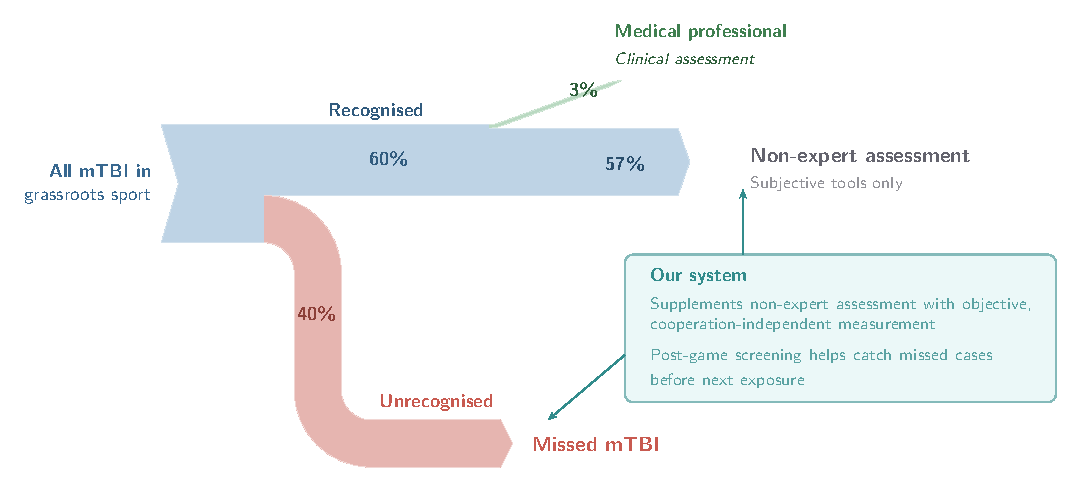
\includegraphics[width=\textwidth]{figures/intro_sankey.pdf}
    \caption{Estimated diagnostic pathway for mTBI in grassroots sport, showing where cases are currently missed. Proportions are approximate; see text for sources and discussion of evidence quality~\cite{mccrea2004unreported, echlin2010sideline, pryor2015athletic}.}
    \label{fig:intro_sankey}
\end{figure}

Mild traumatic brain injury (mTBI)\glsunset{mtbi}, commonly known as concussion, is the most prevalent form of neurological injury worldwide. An estimated 69 million people sustain traumatic brain injury annually~\cite{dewan2019estimating}, of which 70--90\% are classified as mild~\cite{cassidy2004incidence}. Critically, the majority of these injuries occur in community and youth sport settings where no medical professional is present to assess the injured individual.

In these settings, parents, teachers, coaches, and referees often act as de facto first responders yet lack access to objective screening tools. They must rely on visible signs and athlete self-reporting to decide whether medical evaluation is warranted. This approach is inadequate: approximately 50\% of concussions in youth and high school sports go unreported at the time of injury, with athletes failing to recognise the severity of their injury or being unwilling to remove themselves from competition~\cite{mccrea2004unreported, registermihalik2013knowledge}. Athletes routinely minimise symptoms to continue playing, and untrained observers cannot detect subtle neurological dysfunction without quantitative measurement.

The consequences of missed or delayed diagnosis are severe. Second impact syndrome, in which a second head injury is sustained before recovery from the first, causes catastrophic cerebral oedema and brain herniation and is frequently fatal~\cite{sis_statpearls}. Separately, post-concussive syndrome affects up to 15\% of adults following \ab{mtbi}~\cite{ppcs_statpearls}, with up to 50\% of patients symptomatic at three months and 27\% unable to return to their previous level of work at 12 months~\cite{mortaheb2021ppcs}. Early identification is therefore critical to enable appropriate management, prevent premature return to activity, and reduce the likelihood of long-term complications.

These findings establish a clear unmet need: an objective screening capability that can supplement existing non-expert assessment at the point of injury in grassroots sports settings. \Cref{fig:intro_sankey} illustrates this pathway and highlights where cases are currently missed. The 50\% unreporting rate is well-established~\cite{mccrea2004unreported}; bystander detection rates are inferred from video review and instrumented helmet studies~\cite{echlin2010sideline, beckwith2013impacts}, and medical coverage estimates from high school athletic trainer data~\cite{pryor2015athletic}.


\section{Limitations of Existing Approaches}
\label{chapter:introduction:limitations}

Current approaches to \ab{mtbi} assessment fall broadly into two categories: tools that are accessible in field settings but lack objective measurement, and tools that provide quantitative assessment but require clinical infrastructure. Neither addresses the need for objective, point-of-injury screening by non-medical personnel.

\textbf{Accessible but subjective.} The Concussion Recognition Tool 6 (CRT6) was designed specifically for use by non-medical personnel such as parents, coaches, and referees~\cite{echemendia2023crt6}. However, it provides only observational screening without quantitative metrics, requiring the observer to make subjective judgements about concerning signs. More broadly, all field-side assessment approaches that depend on patient self-reporting are vulnerable to symptom minimisation by athletes motivated to return to play. This is not limited to lay observers: athletes systematically underreport symptoms even when assessed by trained team medical personnel, with cleared athletes continuing to minimise symptoms days post-concussion~\cite{meier2015underreporting}. Tools accessible to non-experts thus depend on either patient cooperation or subjective clinical judgement, neither of which provides objective quantitative measurement.

\textbf{Objective but inaccessible.} The \ab{scat6} provides comprehensive evaluation combining symptom inventories, cognitive screening, neurological examination, and balance testing, but requires medical training for proper administration and interpretation~\cite{echemendia2023scat6}. Commercial quantitative pupillometry devices offer objective measurement but cost thousands of pounds and are designed for medical facilities rather than field deployment. The most recent American Congress of Rehabilitation Medicine diagnostic criteria explicitly acknowledge that no validated stand-alone objective diagnostic test is available, even to trained clinicians~\cite{silverberg2023acrm}. Alternative objective biomarkers face different but equally disqualifying limitations: blood biomarkers require venipuncture, laboratory processing, and hours to days of turnaround time, while neuroimaging modalities remain insensitive to the diffuse axonal injury that characterises \ab{mtbi} and require hospital facilities (detailed discussion in \Cref{chapter:background}).

In summary, accessible tools lack objectivity and depend on patient cooperation or subjective assessment, while objective tools require trained personnel, specialised equipment, or clinical infrastructure. No existing approach provides objective quantitative measurement that can supplement non-expert assessment at the point of injury.


\section{Project Objectives}

The analysis in \Cref{chapter:introduction:limitations} establishes four requirements that any effective point-of-injury screening tool must meet:

\begin{itemize}
    \item \textbf{Accessible:} Deployable in grassroots sport settings without specialised medical equipment or infrastructure.

    \item \textbf{Usable by non-experts:} Operable by parents, coaches, and referees without medical training or subjective interpretation.

    \item \textbf{Objective and cooperation-independent:} Provides quantitative measurement that does not depend on patient self-reporting or effort.

    \item \textbf{Rapid:} Completable within 10 minutes, enabling use during or after sporting events.
\end{itemize}

This project develops a headset-based automated pupillometry system designed to \textbf{supplement, not replace,} existing non-expert screening tools such as the CRT6. The rationale for pupillometry as a screening modality is presented in \Cref{chapter:background}; the headset and software design are detailed in \Cref{chapter:headset} and \Cref{chapter:software} respectively.


\section{Scope and Ethical Considerations}

\textbf{Intended use.} The system is a screening instrument, not a diagnostic tool. It identifies individuals who may require further medical evaluation but does not provide a clinical diagnosis of \ab{mtbi}. A negative result does not constitute medical clearance to return to play.

\textbf{Design principles.} In a screening context, the cost of a false negative (a missed concussion) far exceeds the cost of a false positive (an unnecessary referral). The system therefore prioritises sensitivity, and rejects uncertain measurements rather than risks an incorrect result. Hardware and software must be robust to the uncontrolled conditions of field deployment, and application messaging must be clear to non-expert users about what results do and do not mean. The design decisions made to fulfil these criteria are discussed in \Cref{chapter:headset,chapter:software}.

\textbf{Validation limitations.} The system has not been validated on a clinical \ab{mtbi} population. The work presented in this report demonstrates technical feasibility and measurement accuracy on healthy participants. Establishing diagnostic sensitivity and specificity requires future clinical trials with confirmed concussion cases, and any claims regarding diagnostic performance in this report are drawn from the existing literature rather than from our own clinical data.

\textbf{Data privacy.} The system collects oculomotor and biometric data, potentially from minors in sport settings. This carries data privacy obligations under UK GDPR, particularly regarding informed consent, data minimisation, and secure storage. All data collected during testing was handled in accordance with the University's ethical approval procedures. \todo{Detail specific data protection measures implemented (anonymisation, on-device processing, storage protocols).}

\chapter{Technical Background}
\label{chapter:background}

This chapter establishes the scientific foundation for the screening system: it defines \ab{mtbi} and the pathology that resists conventional imaging (\Cref{sec:bg-mtbi}), evaluates existing diagnostic approaches against the screening requirements of \Cref{chapter:introduction} to motivate automated oculomotor screening (\Cref{sec:bg-existing}), details the oculomotor biomarkers underpinning the design (\Cref{sec:bg-oculomotor}), and surveys prior engineering work (\Cref{sec:bg-engineering}).

\section{Mild Traumatic Brain Injury}
\label{sec:bg-mtbi}

\ab{mtbi}, also known as concussion, is defined by the 2023 American Congress of Rehabilitation Medicine criteria as traumatic brain injury with a \ab{gcs} score of 13--15, loss of consciousness lasting less than 30 minutes, and post-traumatic amnesia persisting for less than 24 hours~\cite{silverberg2023acrm}. These thresholds distinguish mild from moderate (\ab{gcs} 9--12) and severe (\ab{gcs} 3--8) TBI. Importantly, the term ``mild'' refers to the initial injury severity classification, not the clinical outcome: a substantial minority of patients experience persistent symptoms and significant disability despite classification as mild~\cite{silverberg2023acrm}.

A primary pathological feature of \ab{mtbi} is \ab{dai}, in which rapid acceleration-deceleration and rotational forces during impact cause widespread microscopic damage to axons~\cite{johnson2013axonal}. Shear forces disrupt axonal microtubules, particularly in white matter tracts such as the corpus callosum, internal capsule, and cerebellar peduncles. This occurs alongside a broader neurometabolic cascade involving ionic flux, excitotoxicity, and neuroinflammation. Unlike focal contusions, \ab{dai} is typically invisible on conventional CT and MRI~\cite{lee2005neuroimaging, palacios2022dti}, motivating screening approaches that do not rely on structural imaging.


\section{Existing Diagnostic Approaches}
\label{sec:bg-existing}

\begin{figure}[b]
    \centering
    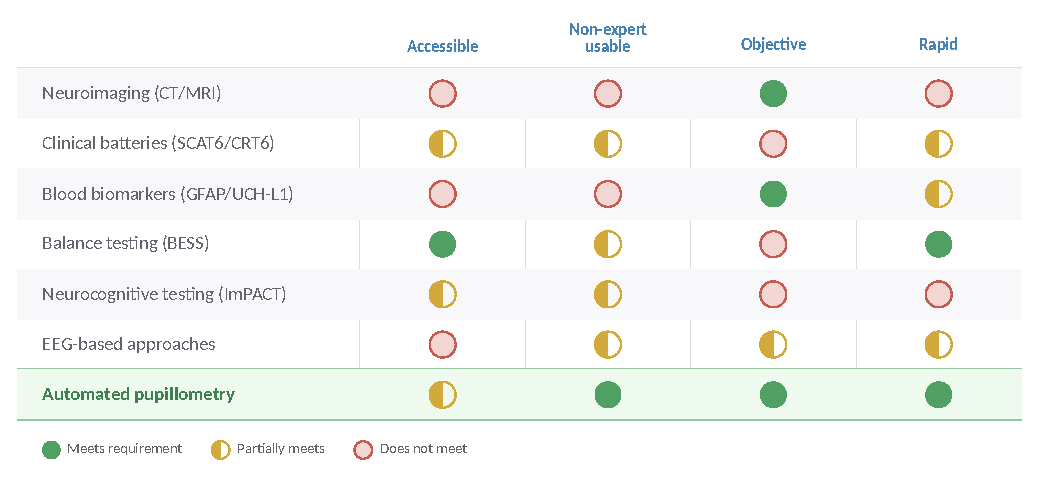
\includegraphics[width=\textwidth]{figures/screening_comparison.pdf}
    \caption{Comparison of candidate mTBI screening approaches against the four requirements identified in \Cref{chapter:introduction}. Automated oculomotor screening most closely satisfies all four criteria, though most existing commercial implementations remain expensive and clinic-based. This accessibility gap is the engineering problem addressed by this project.}
    \label{fig:screening_comparison}
\end{figure}

This section evaluates existing diagnostic approaches against the four requirements of \Cref{chapter:introduction} (\Cref{fig:screening_comparison}) to motivate the choice of automated oculomotor screening.

\textbf{Neuroimaging.} Neuroimaging serves a different clinical purpose to field screening: CT and MRI are used to rule out life-threatening pathology such as intracranial haemorrhage once a patient has reached hospital, not to diagnose \ab{mtbi} at the point of injury~\cite{stiell2001ct, haydel2000ct}. MRI detects abnormalities in approximately 28\% of CT-negative patients~\cite{yuh2013mri}, but most \ab{mtbi} cases remain invisible even on MRI. Advanced diffusion tensor imaging can detect white matter microstructural changes~\cite{palacios2022dti} but remains a research tool. All neuroimaging modalities require hospital infrastructure, specialist operation, and substantial cost.

\textbf{Clinical assessment batteries.} The \ab{scat6} provides structured evaluation combining symptom inventories, cognitive screening, and balance testing, but requires a trained healthcare professional to administer and interpret~\cite{echemendia2023scat6}. The CRT6, designed for non-medical personnel, provides only observational guidance without quantitative metrics~\cite{echemendia2023crt6}. Systematic reviews report highly variable diagnostic performance across assessment components, with sensitivity ranging from 13--92\%~\cite{nelson2013diagnostic}. All such tools depend on either medical training or patient self-report, the latter being vulnerable to symptom minimisation by athletes motivated to continue playing~\cite{meier2015underreporting}.

\textbf{Blood biomarkers.} The FDA-cleared combination of GFAP and UCH-L1 serum biomarkers achieved 97.5\% sensitivity for predicting CT-visible abnormalities, but only approximately 40\% specificity~\cite{bazarian2018blood}. Importantly, these biomarkers are validated for predicting CT findings, not for diagnosing \ab{mtbi} itself. They require venipuncture by trained personnel, laboratory or point-of-care analyser infrastructure, and must be collected within 12 hours of injury. These constraints preclude field deployment by non-medical personnel.

\textbf{Balance and neurocognitive testing.} The Balance Error Scoring System (BESS), commonly used alongside the \ab{scat6}, demonstrates poor sensitivity of only 34\% acutely, declining further over subsequent days~\cite{bell2011bess}. Computerised neurocognitive tests such as ImPACT achieve higher sensitivity (approximately 82\%) but require baseline comparison testing, are vulnerable to deliberate underperformance, and take 20--25 minutes to administer~\cite{schatz2006impact}. Both approaches depend on patient cooperation and physical or cognitive effort.

\textbf{EEG-based approaches.} Quantitative EEG and event-related potential measurements can detect electrophysiological changes following \ab{mtbi}. However, the American Clinical Neurophysiology Society has stated that current evidence does not support the clinical use of quantitative EEG for diagnosing \ab{mtbi}~\cite{nuwer2021qeeg}. Portable systems exist but require electrode application and are sensitive to movement artefact in field environments.

\textbf{Automated oculomotor screening.} Quantitative measurement of the pupillary light reflex and other oculomotor responses provides objective, involuntary biomarkers that do not depend on patient self-report or cooperation. Automated systems require minimal training, can complete assessment in under one minute, and have demonstrated diagnostic accuracy of 91--96\% with machine learning analysis~\cite{maxin2024smartphone}. Automated oculomotor screening therefore satisfies three of the four screening requirements directly: usable by non-experts, objective and cooperation-independent, and rapid. However, most existing commercial systems cost thousands of pounds and are designed for clinical facilities, leaving accessibility as the unresolved engineering challenge this project addresses.

\textbf{Synthesis.} Automated oculomotor screening is the only reviewed approach that satisfies or partially satisfies all four screening requirements (\Cref{fig:screening_comparison}), with accessibility the remaining barrier. The highest published accuracy figures derive from machine learning models validated in specific cohorts, and prospective multi-site validation remains necessary.


\section{Oculomotor Biomarkers}
\label{sec:bg-oculomotor}

Oculomotor dysfunction is observed in 65--90\% of individuals following \ab{mtbi}~\cite{mcdonald2022eye}. This high prevalence reflects the vulnerability of brainstem and midbrain structures to diffuse axonal injury: the oculomotor nucleus, Edinger-Westphal nucleus, and mesencephalic reticular formation all lie in regions particularly susceptible to shearing forces during head acceleration~\cite{hirad2019neural}. This section describes the three oculomotor tests implemented in this system.

\textbf{Pupillary light reflex.} The \ab{plr} is the constriction and subsequent redilation of the pupil in response to light. Constriction is mediated by a parasympathetic pathway from retinal photoreceptors through the pretectal nucleus to the Edinger-Westphal nucleus and via cranial nerve III to the pupil sphincter; redilation is governed by the sympathetic pathway~\cite{ciuffreda2017plr}. \ab{dai} disrupts this pathway at the midbrain level, resulting in measurably altered pupillary dynamics~\cite{bruggeman2020tai}. Multiple \ab{plr} parameters show consistent differences between \ab{mtbi} and control groups, including constriction latency, response amplitude, and recovery time, with eight of nine parameters differing significantly from controls in sport-related concussion and maximum pupil diameter and peak constriction velocity reaching \ab{auc} 0.78~\cite{master2020pupillary, ciuffreda2017plr}.

\textbf{Smooth pursuit.} Smooth pursuit eye movements maintain fixation on a moving target by matching eye velocity to target velocity. The underlying neural pathway spans cortical motion processing areas, pontine relay nuclei, and cerebellar structures, traversing multiple white matter tracts susceptible to \ab{dai}~\cite{mcdonald2022eye, mallott2019cerebellar}. Within 24--48 hours of concussion, athletes show significantly reduced pursuit velocity (Cohen's d = 0.83), with compensatory saccadic intrusions~\cite{murray2019smooth}. Diagnostic discrimination improves further under dual-task conditions: adding a concurrent cognitive load increased \ab{auc} from 0.88 to 0.946~\cite{stubbs2018working}. Smooth pursuit retains discriminative ability for at least 7 days post-injury~\cite{hunfalvay2021smooth}.

\textbf{Vergence.} Vergence eye movements coordinate the eyes to converge or diverge when shifting gaze between near and far targets, controlled by the mesencephalic reticular formation and cerebellar structures~\cite{searle2016vergence}. Convergence insufficiency is one of the most prevalent oculomotor findings following \ab{mtbi}: baseline prevalence in the general population is 2--8\%, rising to 35--49\% acutely post-concussion~\cite{mucha2014voms, pearce2015npc, yaramothu2019vergence, wiecek2021vergence}. Near point of convergence (\ab{npc}) measurement using a threshold of 5 cm achieves an identification rate of 84\%, and combined models incorporating \ab{npc} with other vestibular-ocular measures reach \ab{auc} of 0.89~\cite{mucha2014voms}. Convergence insufficiency also predicts prolonged recovery, with a 12.3-fold increase in odds of recovery exceeding 28 days~\cite{duprey2017convergence}.

\textbf{Multi-modal assessment.} Each of the three biomarkers above probes a different neural pathway, meaning that different patterns of \ab{dai} may affect each test independently~\cite{mcdonald2022eye}. Multi-modal assessment therefore increases sensitivity by detecting abnormality when any single parameter is impaired. Combined oculomotor assessment has achieved 89\% accuracy with 90\% sensitivity and 89\% specificity (\ab{auc} 0.96)~\cite{kelly2019combined}, supporting the multi-parameter approach for screening.

\textbf{Limitations and confounders.} Pupillary responses are influenced by medications (anticholinergics, sympathomimetics, opioids), substance use, and age-related changes including senile miosis and reduced constriction velocity~\cite{mcdougal2015autonomic, huang2024age}. Pre-existing conditions such as physiological anisocoria (present in approximately 20\% of the population), prior eye surgery, and prior TBI can also confound results~\cite{lam1987anisocoria}. For camera-based systems, darker iris pigmentation can reduce the contrast between pupil and iris, complicating boundary detection~\cite{barry2023racially}. Ambient lighting conditions directly affect baseline pupil diameter and must be controlled for reliable measurement. Finally, oculomotor deficits are generally most pronounced in the acute phase and typically resolve over days to weeks, though some can persist beyond symptom resolution~\cite{sussman2016oculomotor}; these confounders inform the hardware and software design choices of \Cref{chapter:headset,chapter:software}.


\section{Engineering Lit Review}
\label{sec:bg-engineering}

\todo{Engineering literature review to be completed.}

\chapter{Hardware}
\label{chapter:headset}

The system is conceived as a low-cost, head-mounted device that standardises the geometry between a user's eyes, a stimulus display, and an imaging sensor in order to perform multi-parameter oculomotor assessment using pupillometry. The headset provides:

\begin{itemize}
    \item A controlled optical pathway from a display to the user's eyes, allowing presentation of pupillary light reflex, smooth pursuit, and vergence stimuli.

    \item A stable, near-frontal view of both eyes for image-based tracking of pupil size and gaze.

    \item A mechanically constrained, repeatable eye--camera distance across users.
\end{itemize}

To remain compatible with deployment in grassroots sports, the design prioritises minimal custom electronics and leverages consumer hardware wherever possible. The headset therefore acts primarily as an optical and mechanical fixture around a smartphone with only simple ancillary electronics (e.g. LEDs) where required.

A key architectural decision is the use of a partially reflective beamsplitter positioned at 45° between the eyes and a display located above the field of view. This beamsplitter performs two functions simultaneously: it reflects the display image into the eyes, mimicking a compact VR headset, and it transmits light from the eyes to a camera located behind the beamsplitter on the same optical axis as the lenses. By keeping the camera bay dark and the display bright, the user perceives only the reflected display image, whilst the camera looks through the beamsplitter at the illuminated eyes. This arrangement resolves the conflict between the need for a straight-on eye view and the requirement that the camera not intrude into the visual field.


\section{Design Criteria}

The hardware must satisfy a set of quantitative and qualitative requirements derived from the clinical use case, the chosen biomarkers, and the intended deployment environment. For clarity, these are grouped into optical, geometric, user-facing, and practical constraints.

\subsection{Optical and Imaging Requirements}

\textbf{Pupil visibility and resolution.} The camera must resolve the pupillary margin sufficiently for accurate segmentation and diameter measurement on each frame. This implies:

\begin{itemize}
    \item Eye region spanning a substantial fraction of the frame (e.g. > 200--300 pixels across the iris for typical smartphone resolutions).

    \item Sufficient contrast between iris and pupil under controlled illumination.
\end{itemize}

\textbf{Viewing angle and distortion.} The camera should view each eye approximately along its optical axis, minimising foreshortening and perspective distortion that would complicate gaze estimation.

\textbf{Controlled illumination.} The optical system must:

\begin{itemize}
    \item Provide enough light to achieve low-noise images at video frame rates.

    \item Avoid large specular glares that obscure the pupil.

    \item Support controlled light stimuli for PLR (rapid change in illumination) without saturating the sensor or causing discomfort.
\end{itemize}

\textbf{Stimulus--eye relationship.} The geometry between the eye and the display must be known and stable so that the position of a dot or other stimuli on the screen can be related to an expected gaze direction.

\subsection{Geometric and Mechanical Requirements}

\textbf{Fixed eye--camera distance.} The headset must constrain the distance and relative orientation between eyes and camera to within a tight tolerance across users (e.g. variations on the order of a few millimetres), ensuring that calibration performed once is valid for repeated tests.

\textbf{Accommodation comfort.} The virtual distance of the viewed image must fall within a comfortable accommodative range for children and adolescents, and must not induce significant eye strain during testing.

\textbf{Alignment repeatability.} The design should assist users in positioning the headset correctly (e.g. via nose bridge, straps, and padding) so that the eye-box (region where both eyes see the full display and are fully visible to the camera) is easy to locate.

\subsection{User-Facing Requirements}

\textbf{Comfort and safety.} The headset must be lightweight, distribute pressure evenly, avoid sharp edges, and be tolerable for a few minutes of use immediately after a suspected head injury.

\textbf{Low cognitive and visual load.} Optical design should avoid unusual or distracting artefacts (e.g. a visible camera in one eye) that could be unsettling, especially for symptomatic users.

\subsection{Practical and Economic Requirements}

\textbf{Low cost.} The bill of materials (excluding the user's smartphone) should fall in the £30--£80 range, precluding the use of multiple high-speed IR cameras or custom microdisplays.

\textbf{Robustness and manufacturability.} Components should be readily available, mechanically robust, and tolerant of repeated handling in school and club environments.

\textbf{Modularity.} The design should permit substitution of different smartphones (within a size range) and potential future upgrades (e.g. adding IR LEDs) without complete redesign.

These requirements guided the exploration of candidate optical and mechanical configurations.


\section{Optics}

\subsection{Direct Viewing Without Lenses}

A natural baseline configuration places the display at a distance where users can focus without additional optics, and positions the camera near the display to observe the eyes. A prototype implementing this concept used a smartphone screen at distances in the range 20--30~cm from the eyes, mounted within an extended headset ``tube''.

Informal testing with multiple users showed that whilst some individuals could accommodate at these distances, others struggled to achieve a clear image or reported rapid onset of eye strain. Reported comfortable focus distances varied substantially between users, and increasing the display distance to accommodate those with poorer near vision produced an impractically large form factor.

This approach failed several requirements:

\begin{itemize}
    \item \textbf{Accommodation comfort and variability.} The design relied on the user's accommodative ability at relatively close distances, producing an unacceptable spread in user experience and risking exacerbation of symptoms in recently concussed individuals.

    \item \textbf{Form factor.} Achieving a universally comfortable focus distance without optics implied a very deep headset, undermining portability and comfort.
\end{itemize}

These results motivated the introduction of lenses to decouple the physical display distance from the perceived focus distance.


\subsection{Formal Justification for Lenses}

\todo{Need lenses for 3D image, which is needed for convergence testing. Analyse the impact of losing convergence testing.}

\todo{Need lenses to be able to position the display nearer than the user's near point without inducing eye-strain or blurry vision. This is necessary otherwise we get an impractically long headset.}


\subsection{Camera Positioning}

\todo{Once the need for lenses has been established, it is useful to consider conventional VR setups, particularly in the context of camera placements. Meta Pro and Apple Vision Pro both have...}


\section{Electronics}

% TODO: Describe electronics design
% - LED illumination
% - PCB design
% - Communication protocols
% - Power management


\section{Ergonomics and Assembly}

The headset must be comfortable for potentially concussed individuals, robust enough for repeated use in grassroots sport settings, and hygienic for sharing between athletes.

\textbf{Material.} The shell is 3D printed in PETG, chosen as a compromise between printability, mechanical properties, and suitability for skin contact. PLA was considered but rejected due to brittleness under impact and a low heat deflection temperature ($\sim$55\textdegree C), making it unsuitable for equipment stored or transported in warm environments~\cite{tymrak2014mechanical}. PETG offers comparable print quality to PLA with substantially better impact resistance, chemical resistance to common cleaning agents, and adequate thermal tolerance ($\sim$70\textdegree C)~\cite{tymrak2014mechanical}. For a production device, Nylon PA12 would be preferred: it is approximately 15--20\% lighter by volume than PETG, offers superior fatigue and abrasion resistance, and is ISO 10993 certified for skin-contact medical devices~\cite{bazan2023pa12}. However, PA12 requires an enclosed print chamber and dry filament storage, making it impractical for rapid prototyping iterations.

\textbf{Strap system.} A three-point elastic strap system (two side straps and one top strap) meets at a padded rear cradle at the occipital bone. This configuration was selected over a halo strap (over-engineered for sub-10-minute use and slower to don) and a simple elastic band (inadequate stability, all load on cheeks). The top strap is critical: it converts the forward torque from the front-mounted optics into a distributed upward force across the crown, preventing the headset from sliding down the face. A rear adjustment mechanism accommodates head circumferences from children aged 10 through adult. Donning time targets under 10 seconds to minimise delay during a screening assessment.

\textbf{Weight and centre of mass.} The complete assembly targets a total weight under 200 g, comparable to a pair of ski goggles and well within the comfort range for short-duration use. At this weight class, research indicates that neck torque is not a significant factor for sessions under 10 minutes, and counterweights are unnecessary~\cite{odell2024weight}. The centre of mass is kept within 2--3 cm anterior to the eyes by minimising the depth of the optical path, following ergonomics research showing that anterior displacement of the centre of mass significantly increases cervical spine loading at higher device weights~\cite{astrologo2024hmd, chihara2018workload}. \todo{Add actual measured weight and CoM position from final prototype.}

\textbf{Facial interface and hygiene.} The facial interface uses PU leather-covered closed-cell foam, 8--10 mm thick, attached to the shell via a snap-fit mechanism for easy removal. PU leather was selected over open-cell foam (which absorbs sweat and harbours bacteria) and silicone (higher cost, though preferable for a production device). The interface is wipeable with alcohol-free antibacterial wipes between uses. The shell itself is sanded and sealed to reduce the porosity inherent in FDM printing, preventing bacterial accumulation on the device body. A cleaning protocol is provided with the device. \todo{Specify cleaning protocol details.}

\textbf{Light sealing and ventilation.} Consistent pupillary light reflex measurement requires controlled ambient light conditions, as identified in \Cref{sec:bg-oculomotor}. The facial interface provides a light seal around the eyes, blocking external illumination. However, a fully sealed enclosure causes fogging of the beamsplitter and lenses from breath and body heat, degrading image quality. This is addressed by incorporating small baffled vents at the lower edge of the headset: the baffles admit airflow while blocking direct light paths. The vents are positioned below the optical axis to prevent light ingress from reaching the camera sensor. \todo{Verify vent design in final prototype.}

\textbf{Robustness.} The device is intended for use in school and club environments where it will be transported in kit bags and handled by non-experts. PETG's impact resistance provides adequate drop protection for the prototype; a production device in PA12 would improve this further. All optical components (beamsplitter, lenses, camera module) are recessed within the shell rather than exposed, protecting them from accidental damage. \todo{Add figure: annotated CAD render showing key features, and side-view diagram showing centre of mass position.}

\chapter{Software}
\label{chapter:software}

\section{System Overview}

The headset is designed such that the Raspberry Pi~5 CPU must run a stimulus display, two 120\,fps camera streams, an IMU polling loop, Bluetooth communication, and edge inference. The software described in this chapter manages these concurrent workloads and implements the full pipeline from raw sensor data to a trial result, covering model training, real-time inference, signal quality filtering, metric extraction, and secure data handling. The software builds on the biomarker analysis in \Cref{chapter:background} and the hardware in \Cref{chapter:headset} to implement the full pipeline from sensor data to trial result.

Separate machine learning models were fine-tuned for each of these biomarkers. For smooth pursuit, a convolutional neural network (CNN) was developed which, given an image, determines the angle of an eye, helping to assess whether a user can follow a marker on a screen properly. For the pupil light reflex biomarker, a different CNN model measures pupil width, giving insight into pupil dilation responses when exposed to light by producing a binary mask that shows whether a pixel belongs to the pupil or not.

The software was designed to ensure that it led to a trial that was robust, giving accurate, repeatable, and reliable results whilst preserving data security as per GDPR and HIPAA compliance~\cite{ico_gdpr_minimisation, hhs_hipaa_privacy}. These constraints led to the design philosophy of simple, validated methodologies that will be reused with hardware iterations and further data collection. This shaped our choices throughout this chapter such as FP32 before INT8 quantisation, using synthetic pursuit trajectories before real trial data, deferring optimisation in favour of buildability, and documenting the path to a more accurate version once the system is more stable with test data available.

To ensure that users can easily operate this system, a phone app controls the headset and displays results. A simple interface lowers the risk of them not wanting to undergo a test due to operating friction, increasing user safety. \Cref{fig:app-design} shows the design of the app which will be developed.

\begin{figure}[htbp]
    \centering
    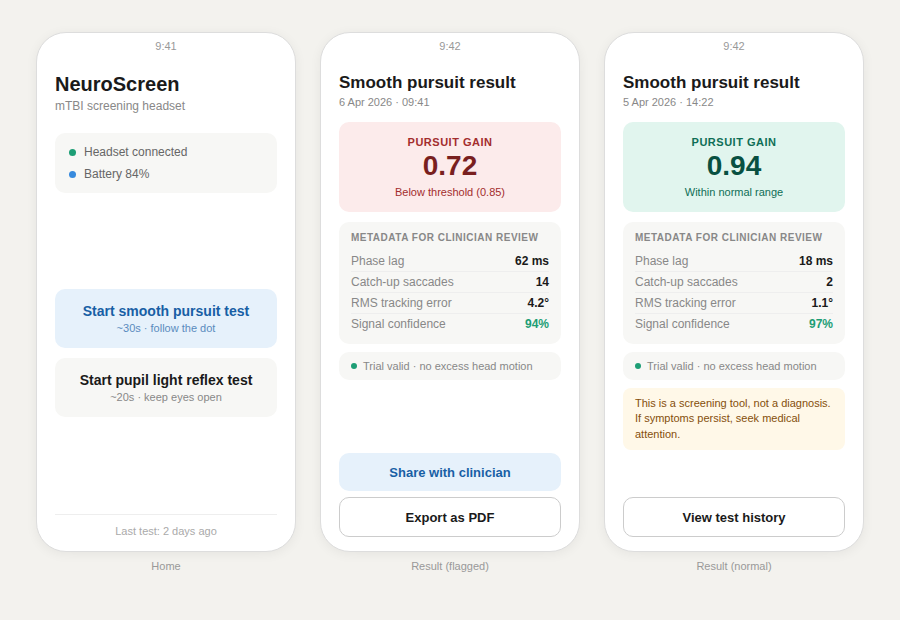
\includegraphics[width=\textwidth]{figures/app_design}
    \caption{App design for controlling the headset.}
    \label{fig:app-design}
\end{figure}

\section{On-Device Inference: LiteRT (formerly TensorFlow Lite) Runtime}

We decided on using LiteRT for the inference engine. A runtime shapes the system's latency, memory footprint, energy consumption, and operational reliability. Simultaneously running with the model are the stimulus display, IMU polling loop, Bluetooth communication, and the cameras. These system conditions paired with the fact that the models run entirely on the Pi~5 show that it is extremely important that an appropriate runtime is selected around our design choices and system philosophy.

The three inference backends evaluated for deploying MobileNetV2 on the Pi~5's Broadcom BCM2712 SoC were: PyTorch, ONNX Runtime, and LiteRT.

PyTorch was not selected as the inference engine since its main function is as a training and research framework rather than a lightweight inference engine. The PyTorch Pi tutorial shows that real-time inference on the Pi~5 is feasible, but considering it will be purely doing forward inference, the full framework is a heavier solution than necessary. ONNX Runtime, however, was intentionally engineered as an inference-focused runtime with a documented Raspberry Pi deployment path and an official edge tutorial, showing it to be a serious option~\cite{onnxruntime2021}.

This is further implied in research comparing the energy consumption of PyTorch versus LiteRT and ONNX Runtime~\cite{malenza2025energy}, showing that ONNX and LiteRT are more energy-efficient on MobileNetV2 for CPU workloads. This paper was on different hardware, however, so more specific benchmarking on the Pi~5 is needed to fully support this statement.

Furthermore, benchmarking on Pi ARM hardware shows that the runtime choice affects inference performance, with LiteRT performing strongly, especially when using INT8 quantisation~\cite{baller2021deepedgebench}. ONNX is frequently used in edge inference devices, with both LiteRT and ONNX being appropriate choices for inference on the Pi, with the final selection depending on future quantisation plans.

At FP32 inference the literature is ambiguous. This was resolved through benchmarking the runtimes on an Apple Silicon ARM CPU using four threads and FP32 precision to display approximately 1.2$\times$ better performance from LiteRT. Apple Silicon is not the Pi~5, with its cache hierarchy and SIMD width differing from the Cortex-A76 cores in the BCM2712, so the absolute latencies are not transferable and the relative rankings have their limitations too. Despite this, both use the ARM instruction set and these rankings are reinforced by trends seen in the literature~\cite{baller2021deepedgebench}.

\begin{table}[htbp]
    \centering
    \caption{Runtime benchmark comparison for MobileNetV2 FP32 inference on Apple Silicon ARM (4 threads, 200 passes, 30-iteration warmup).}
    \label{tab:runtime-benchmark}
    \begin{tabular}{lcccc}
        \toprule
        \textbf{Runtime} & \textbf{Mean Latency} & \textbf{P95} & \textbf{FPS} & \textbf{Model Size} \\
        \midrule
        \textbf{LiteRT (TFLite)} & \textbf{2.68\,ms} & 2.85\,ms & 373 & 11.5\,MB \\
        ONNX Runtime             & 3.23\,ms           & 3.82\,ms & 309 & 0.3\,MB \\
        PyTorch                  & 22.35\,ms          & 23.71\,ms & 45 & 12.0\,MB \\
        \bottomrule
    \end{tabular}
\end{table}

\Cref{tab:runtime-benchmark} shows that LiteRT achieves the best performance. Based on these results and the potential for future INT8 quantisation, LiteRT was selected as the more future-proof choice.

\subsection{Future Improvement and Current Limitations}

The present software uses FP32 deployment to avoid introducing quantisation errors in the gaze estimation pipeline. A future optimisation could be INT8 quantisation, which would cause the CPU inference efficiency to increase as the model size would reduce by approximately $4\times$. Further consideration would have to be put in how quantisation is done, as in MobileNet architectures post-training quantisation (PTQ) can cause large accuracy degradation~\cite{yun2021mobilenets}, whereas quantisation-aware training (QAT) is specifically designed for preserving accuracy~\cite{google_qat} by exposing the model to the effects of quantisation during the training process. This shows that although INT8 quantisation is attractive for constrained resources, the accuracy penalty must be properly controlled via careful quantisation methods. FP32 was therefore chosen for simplicity to achieve validation, with future software updates possibly including INT8 QAT optimisation. This reflects the intentions of the engineering philosophy concerning a simple and reliable baseline, where further optimisations can be brought in later.

\section{Smooth Pursuit Trial}

Smooth pursuit eye movement issues can occur with mTBI, as discussed in depth in \Cref{chapter:background}. Smooth pursuit dysfunction is a reliable indicator for underlying mTBI issues and specifically causes:

\begin{enumerate}
    \item \textbf{Saccadic jumps:} the eyes fall behind the object being watched and then jump forward to catch up.
    \item \textbf{Latency:} a delay between when the object starts moving and when the eyes start to follow it.
\end{enumerate}

The software in this section implements the smooth pursuit assessment pipeline for the headset hardware. For this trial, the user must follow a moving marker on the display screen moving sinusoidally horizontally. The camera collects the images of the eye, and the gaze estimation is compared with the ground truth angle from the marker to develop a set of metrics to assess if there are underlying pursuit issues. If they have smooth pursuit issues, the latencies and saccadic jumps will appear. Strong software was developed to use the data collected from the sensors to train a robust machine learning model and filter the outputs during testing so that truthful metrics can be extracted, producing meaningful and reliable results.

\subsection{Smooth Pursuit Metrics}

The metrics that were chosen are:

\begin{enumerate}
    \item \textbf{Pursuit gain:} Calculated through taking the FFT of both signals, as the target motion is sinusoidal, analysing the amplitudes at the stimulus frequency. Gain is defined as Amplitude$_{\text{eye}}$ / Amplitude$_{\text{target}}$. This should be close to unity, with lower values suggesting poor performance~\cite{devillerssidani2023oculomotor}.

    \item \textbf{Catch-up saccade activity:} The algorithm first calculates the eye velocity from the gaze estimation signal and detects the saccades where the velocity exceeds a threshold, retaining only the events which occur whilst the eye is behind the target and the jump reduces the tracking error~\cite{devillerssidani2023oculomotor}.

    \item \textbf{RMS tracking error:} The root-mean-square difference between the measured eye angle and the expected target angle~\cite{kellar2018comparing}.

    \item \textbf{Motion validity and signal confidence:} The module also outputs two quality-related quantities. Motion validity is derived from IMU-based gating logic and indicates whether excessive head movement compromised the trial. Signal confidence reflects the reliability of the eye-tracking signal, derived from analysis of blur, blinking, and glare.

    \item \textbf{Lag:} Calculated through the cross-correlation between the gaze estimation and ground truth signal, finding the time offset which maximises the correlation peak. This is consistent with prior work in which pursuit lag is treated as a key parameter~\cite{devillerssidani2023oculomotor}.
\end{enumerate}

These metrics are used to determine trial validity. The trial is disqualified if the IMU acceleration exceeds 1.5\,g for more than 300\,ms, or if more than 10\% of frames are rejected by the quality pipeline. These provisional thresholds will be revised against real headset data.

Gain was decided as the core metric for the trial result as it is the most clinically established metric~\cite{leigh2015neurology}, with the other metrics passed as metadata. The gain threshold was set at 0.85. At low stimulus frequencies ($\leq$0.4\,Hz), healthy horizontal pursuit gain is 0.9--1.0~\cite{meyer2020smoothpursuit}; 0.85 sits just below this range, giving noise tolerance without sacrificing sensitivity to genuine deficits. Metadata is provided so that clinicians can make more well-informed decisions about next steps, ensuring ethical considerations protect against false results such as false negatives.

\section{Data Collection Pipeline}

For training and testing, the data streams recorded are the display angle, the timestamps, the IMU motion stream, the quality indicators of the eye signal, and a signal derived from the eye. This derived signal is the raw eye image if collecting for training, and the predicted gaze angle if for testing.

The core difference is that in training mode the goal is to collect images of the eyes with the ground truth angle, and in testing, the goal is to collect the images of the eyes to determine an estimated gaze angle, comparing against the ground truth display angle to understand whether there are underlying smooth pursuit issues.

The data retention schemes for either are hence very different. In training, the system retains raw eye imagery together with the timeseries, event logs, and session metadata. Data is written locally in buffered chunks of 5~seconds, uploaded via WiFi due to system requirements, and then deleted shortly after to preserve memory. This was an engineering tradeoff as too long would mean a high risk of data loss if there is upload delay, and too frequent transfer would cause large transfer overhead.

In testing, the system stores the aligned timeseries, extracts the pursuit metrics, session metadata, and the final trial result, discarding the raw eye video after calculating the image confidence score and the estimated gaze angle. Image data is deleted as 120\,fps is storage intensive at approximately 2\,GB per 30-second session. The compact 5\,kB result is then transmitted to the user's phone via Bluetooth whilst caching the session summary until there is successful transfer, in case of sparse connectivity. Further evidence for this method is seen in research reflecting an edge-computing architecture where sensitive data is processed and stored locally first, with deferred bulk transfer used to reduce the real-time bandwidth and latency requirements so sensitive data is not transmitted over the network~\cite{rancea2024edge}.

Sustainability, IP, and security: These decisions were more environmentally friendly as edge computing is more carbon efficient than cloud computing~\cite{ma2025greening}. Immediately deleting the images and encrypting the wireless transmissions also help with minimising storage footprint and protecting the user's IP and security, under GDPR, CCPA, and HIPAA compliance. These principles can also be carried through in future iterations, extending useful life through keeping old practices.

\begin{figure}[htbp]
    \centering
    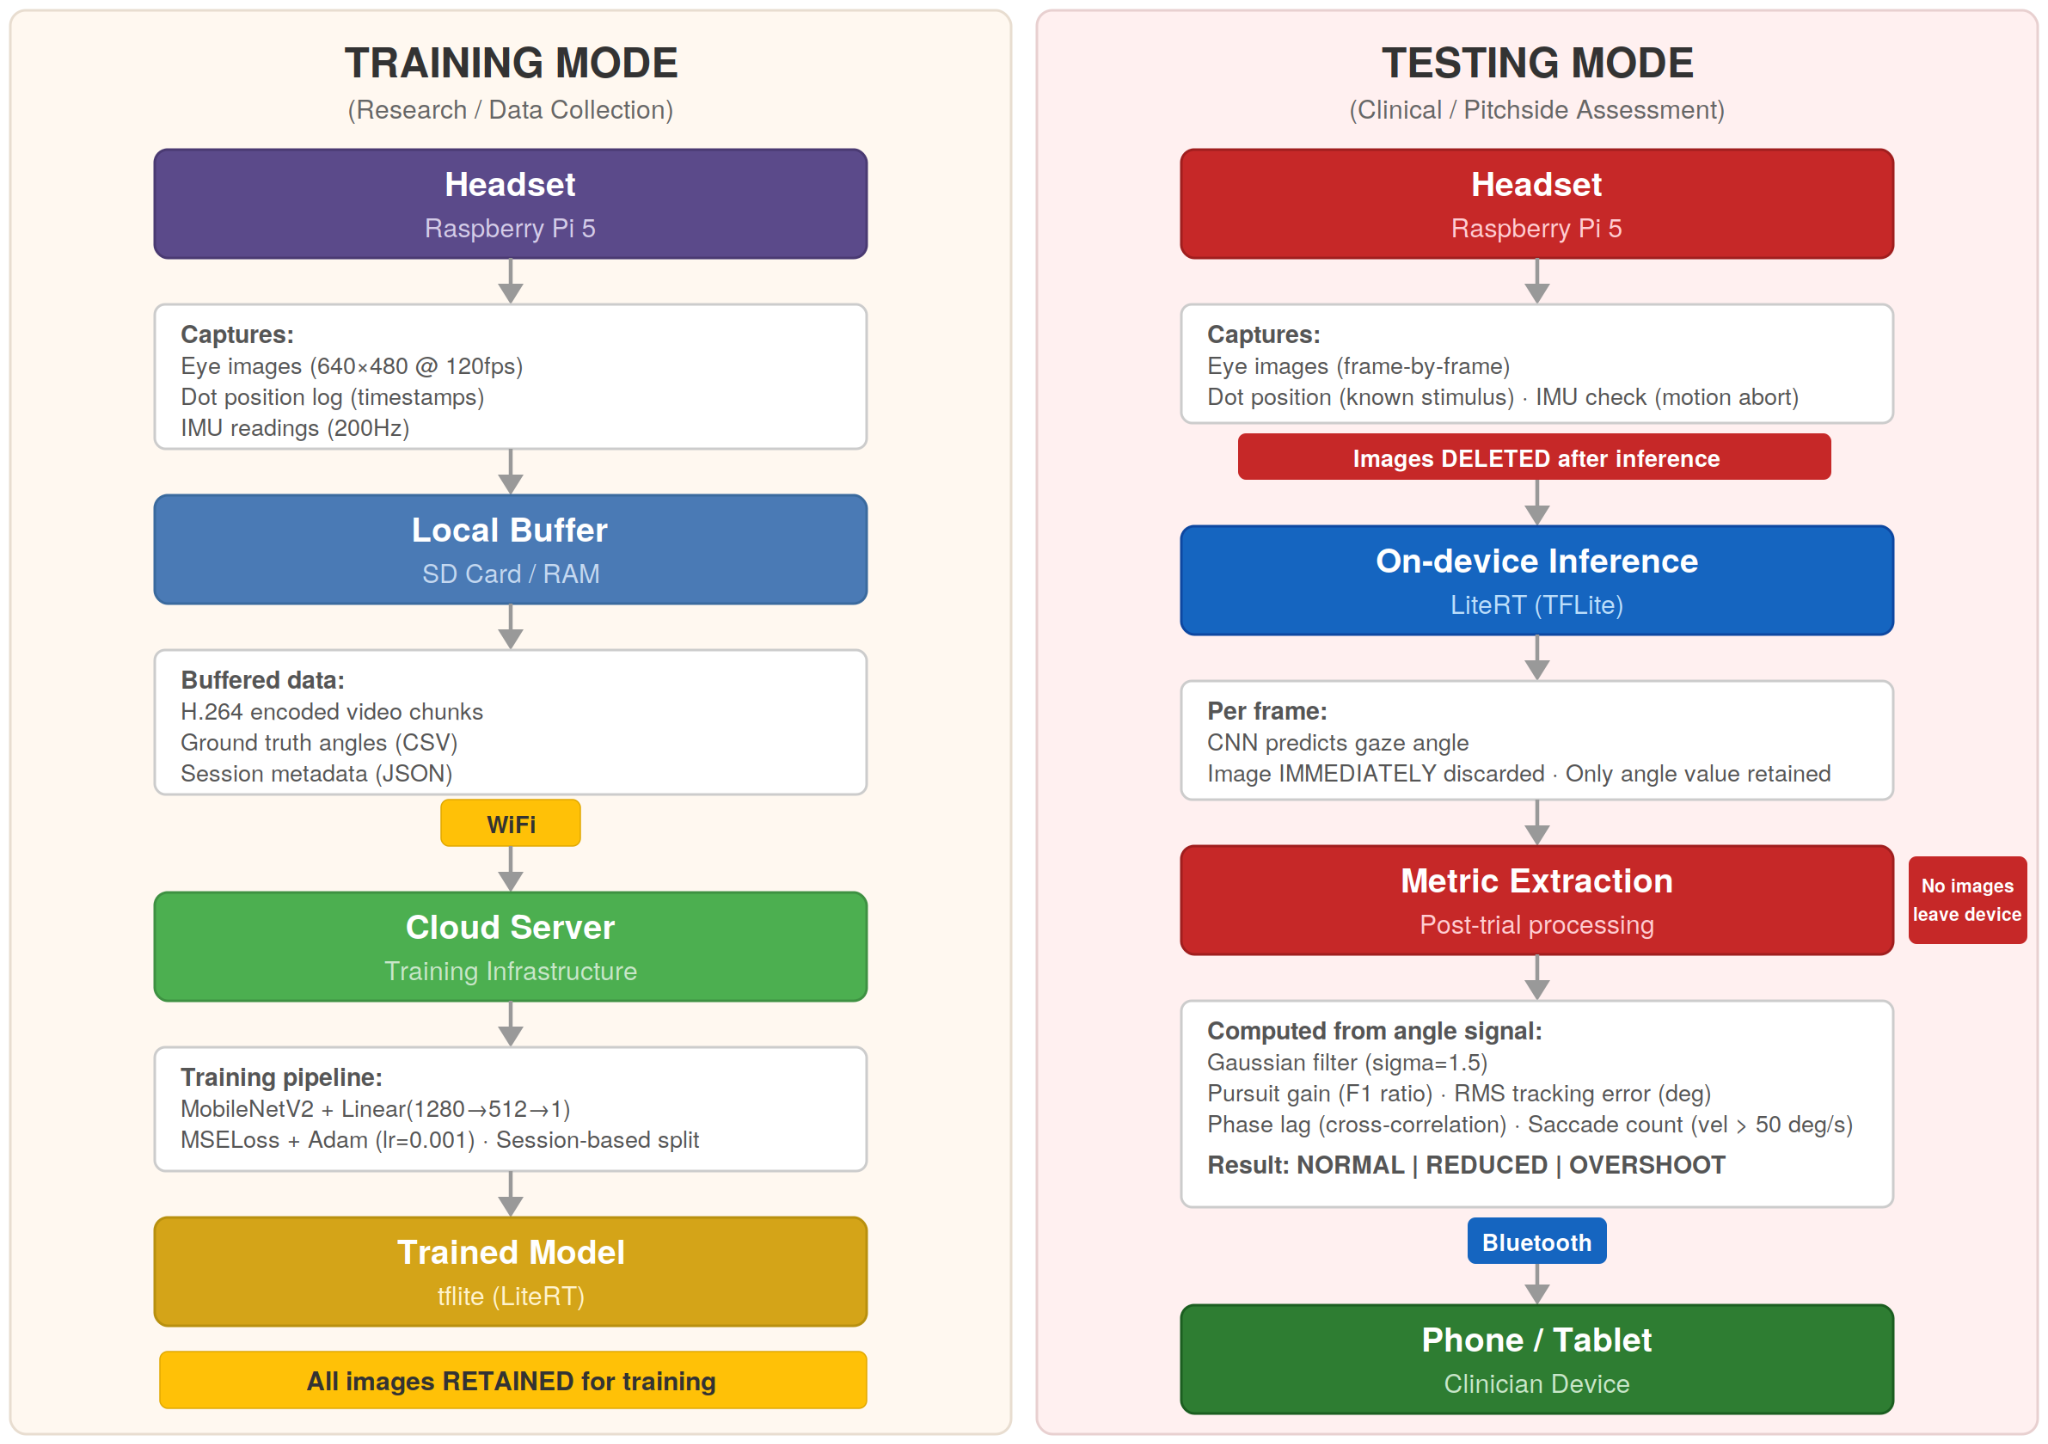
\includegraphics[width=\textwidth]{figures/data_pipeline}
    \caption{Data flow in the smooth pursuit trial, showing the training and testing paths.}
    \label{fig:data-pipeline}
\end{figure}

Both modes require synchronisation between the ground truth signal and the gaze estimation or image signal. In this prototype they are aligned through the monotonic software clock rather than by calibrating hardware latencies (sensor to CPU delay, screen render delay). Hardware calibration will be done in later hardware iterations.

\section{Testing Technologies}

When raw data is collected from the sensors and the gaze estimation model, it is important that it is cleaned so inference is accurate and the results are reliable. Regions of low confidence will exist in the gaze estimation due to blur, glare, and blinking. Removing these is important as they can poison metrics and give misleading results, carrying a risk of potential false negatives. Filtering is also necessary so that artifacts of noise which imitate poor pursuit performance are removed, letting us uncover the true gaze signal. This is predominantly saccade count as the noise imitates its characteristics, with catch-up saccade detection being the most noise-sensitive downstream metric~\cite{birawo2022review, leube2017sampling, cheng2026eye}. Unlike gain or RMS tracking error which are computed over longer temporal windows, the saccadic activity depends on brief high-velocity events and is therefore far more vulnerable to peaks. Simultaneously, over-filtering must be avoided as it can remove the original signal artifacts.

The model outputs gaze angles without confidence estimates; uncertainty-aware gaze regression is shown~\cite{kendall2017uncertainties, kuleshov2018accurate} to produce unreliable calibration, so image quality metrics such as blur and glare are used for external gating instead.

\subsubsection*{Blur and Blinking Detection}

The Laplacian of the image was analysed for detecting blur and blinking, having chosen a value of 1.6 as the cutoff with all values $\leq$~1.6 rejected. Blinking presents images similar to blur so the same algorithm is reused.

\begin{figure}[htbp]
    \centering
    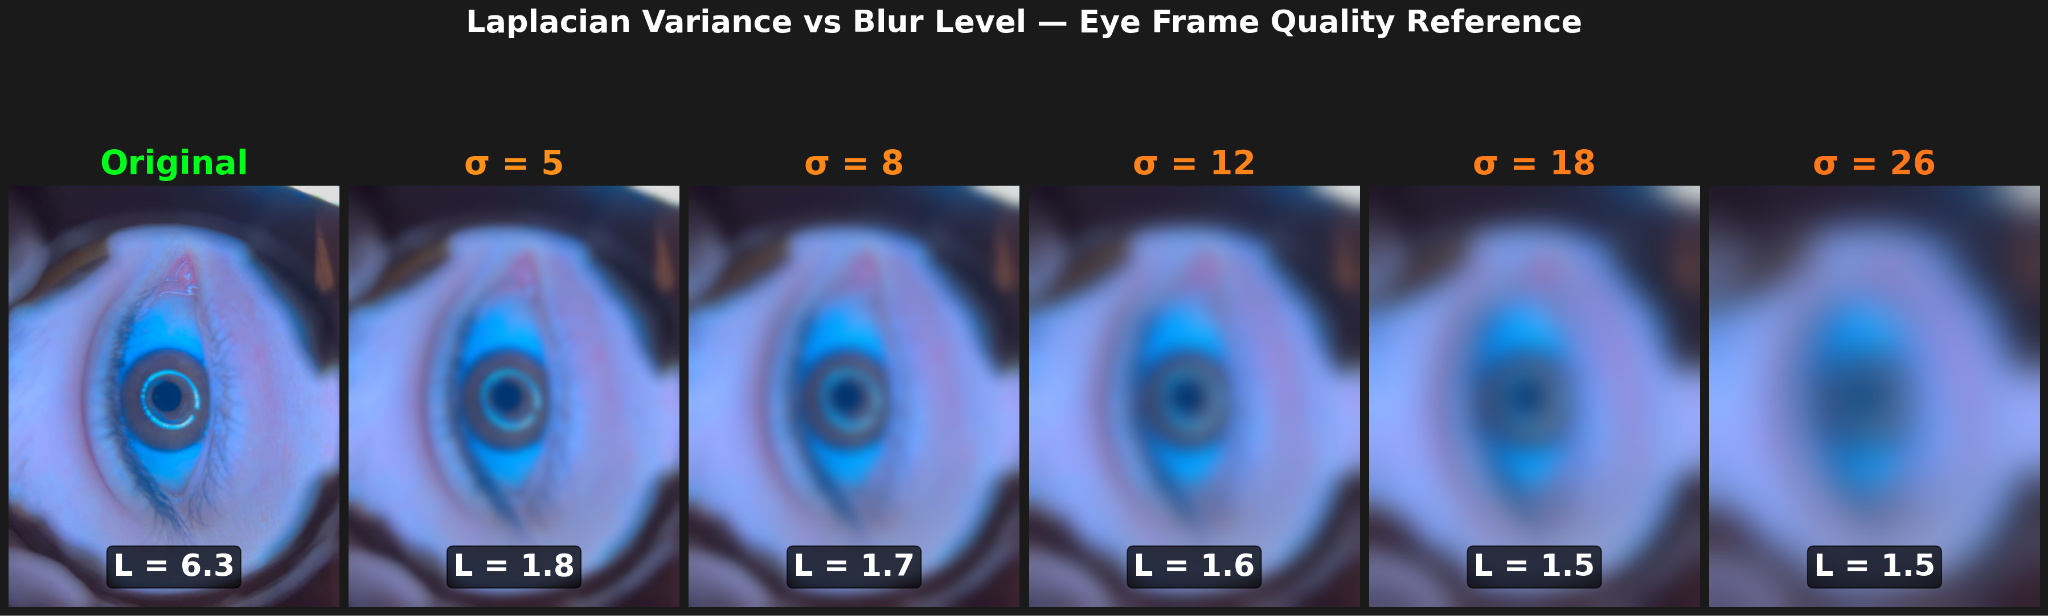
\includegraphics[width=\textwidth]{figures/blur_blink_detection}
    \caption{Blur and blinking---Laplacian variance vs blur level.}
    \label{fig:blur-blink}
\end{figure}

\subsubsection*{Glare Detection}

Glare detection involves analysing the saturated pixel ratio, choosing a value of 1\% as the cutoff so there is still room for glare whilst not poisoning our metrics, giving a balance of accuracy and practicality.

\begin{figure}[htbp]
    \centering
    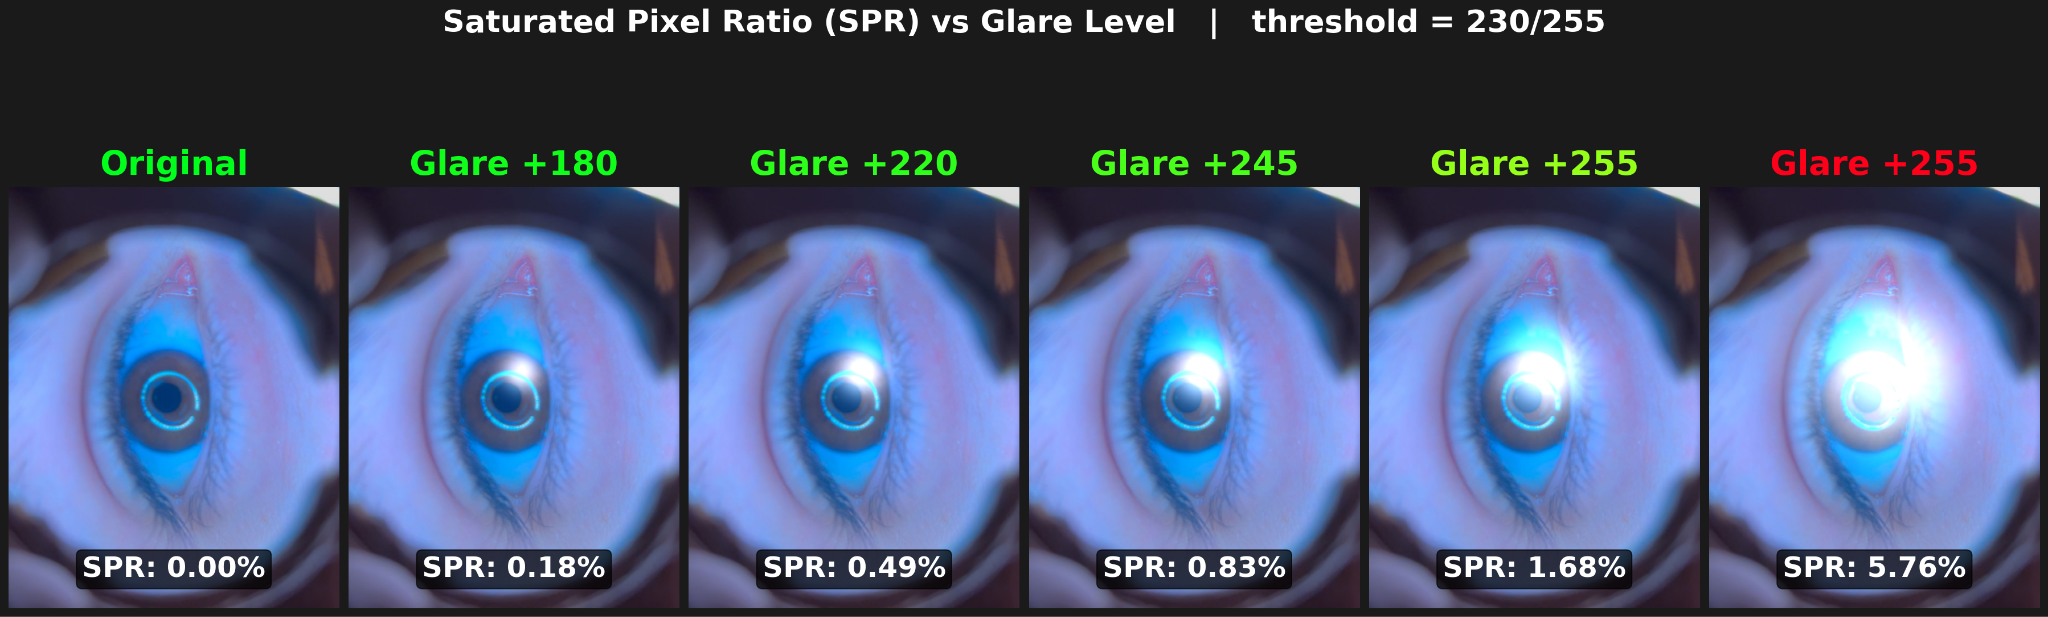
\includegraphics[width=\textwidth]{figures/glare_detection}
    \caption{Glare detection from 0\% to 5.758\% saturated pixel ratio.}
    \label{fig:glare}
\end{figure}

These thresholds outlined produced a risk mitigation strategy against false negatives, a dangerous failure mode prevented under ethical considerations.

\subsubsection*{Filter Selection}

The filter is to preserve genuine pursuit deficits whilst rejecting noise-induced artifacts. This methodology is validated on synthetic data so that the approach can be reused with real noise statistics once headset data is available. To fulfil this, synthetic pursuit trajectories were created from the ideal pursuit with no issues to the worst, increasing the saccade count each time. A comparison was then made between the true saccade count with the calculated one from the filtered signal to see which filter could reproduce the metrics most accurately, using sigma~$=$~0.6 noise addition between these as the test parameter. Saccades were used to guide the filter performance as it is the most noise-sensitive downstream metric, further supported in eye movement detection literature because saccades are detected using velocity-threshold algorithms~\cite{birawo2022review}, making them even more prone to noise after differentiation. Hence, this process was tuned against the most fragile part of the metric pipeline as the filter should then be adequate for the other slower, lower-frequency measures such as gain and RMS tracking error~\cite{birawo2022review}.

\begin{figure}[htbp]
    \centering
    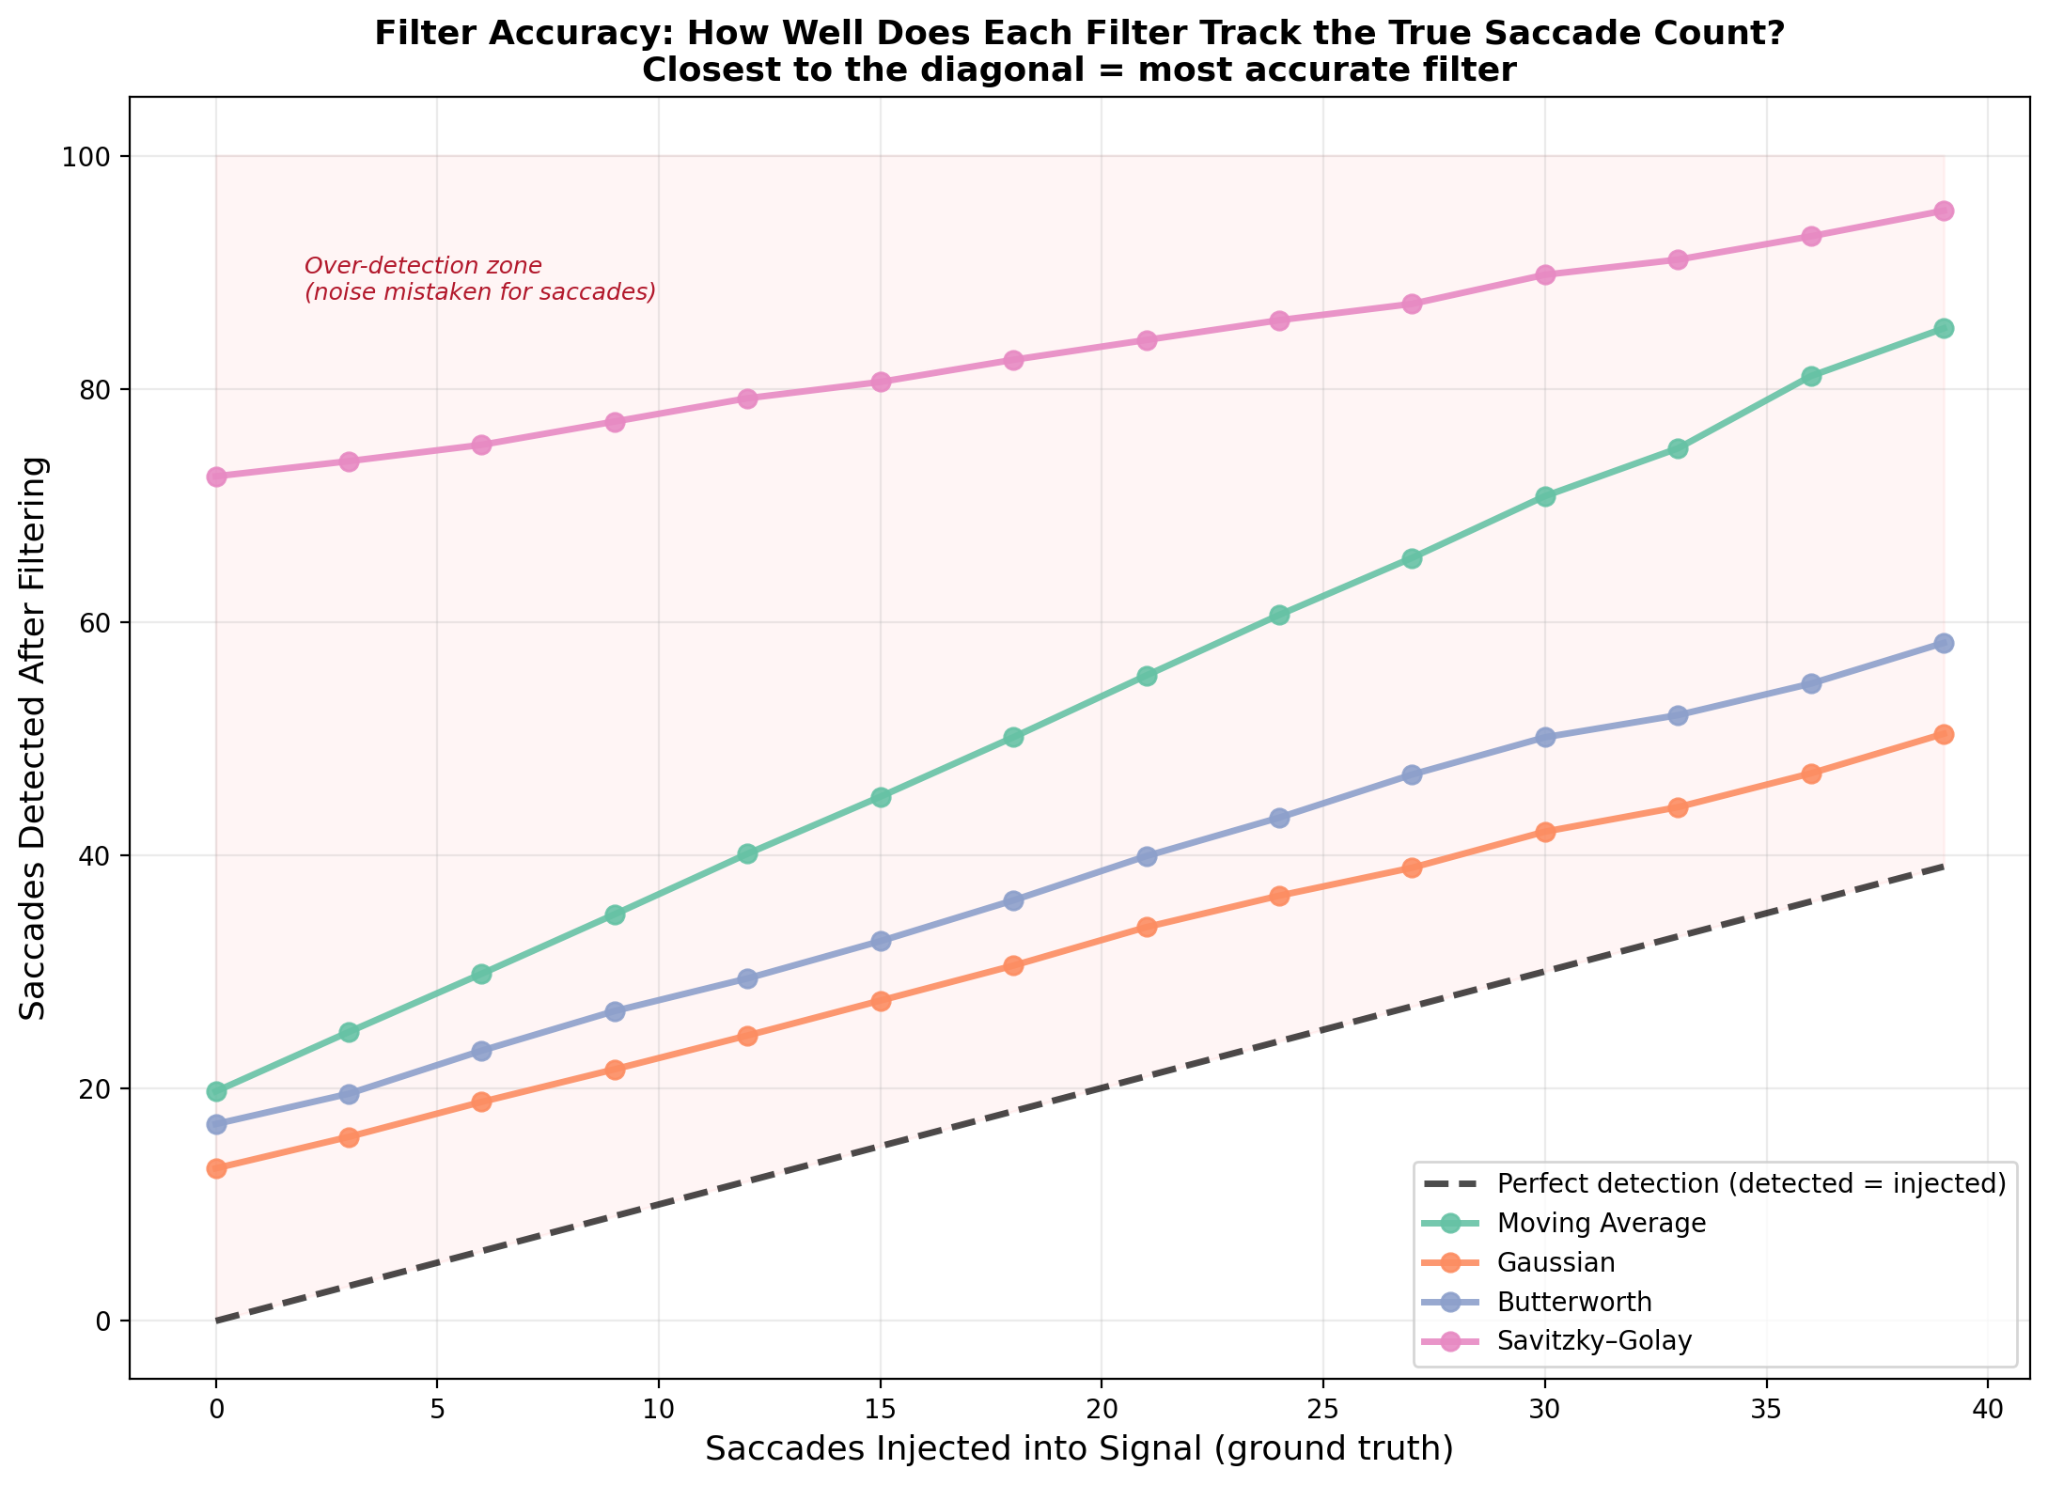
\includegraphics[width=\textwidth]{figures/filter_comparison}
    \caption{Gaussian filter performance comparison.}
    \label{fig:filter-comparison}
\end{figure}

\begin{figure}[htbp]
    \centering
    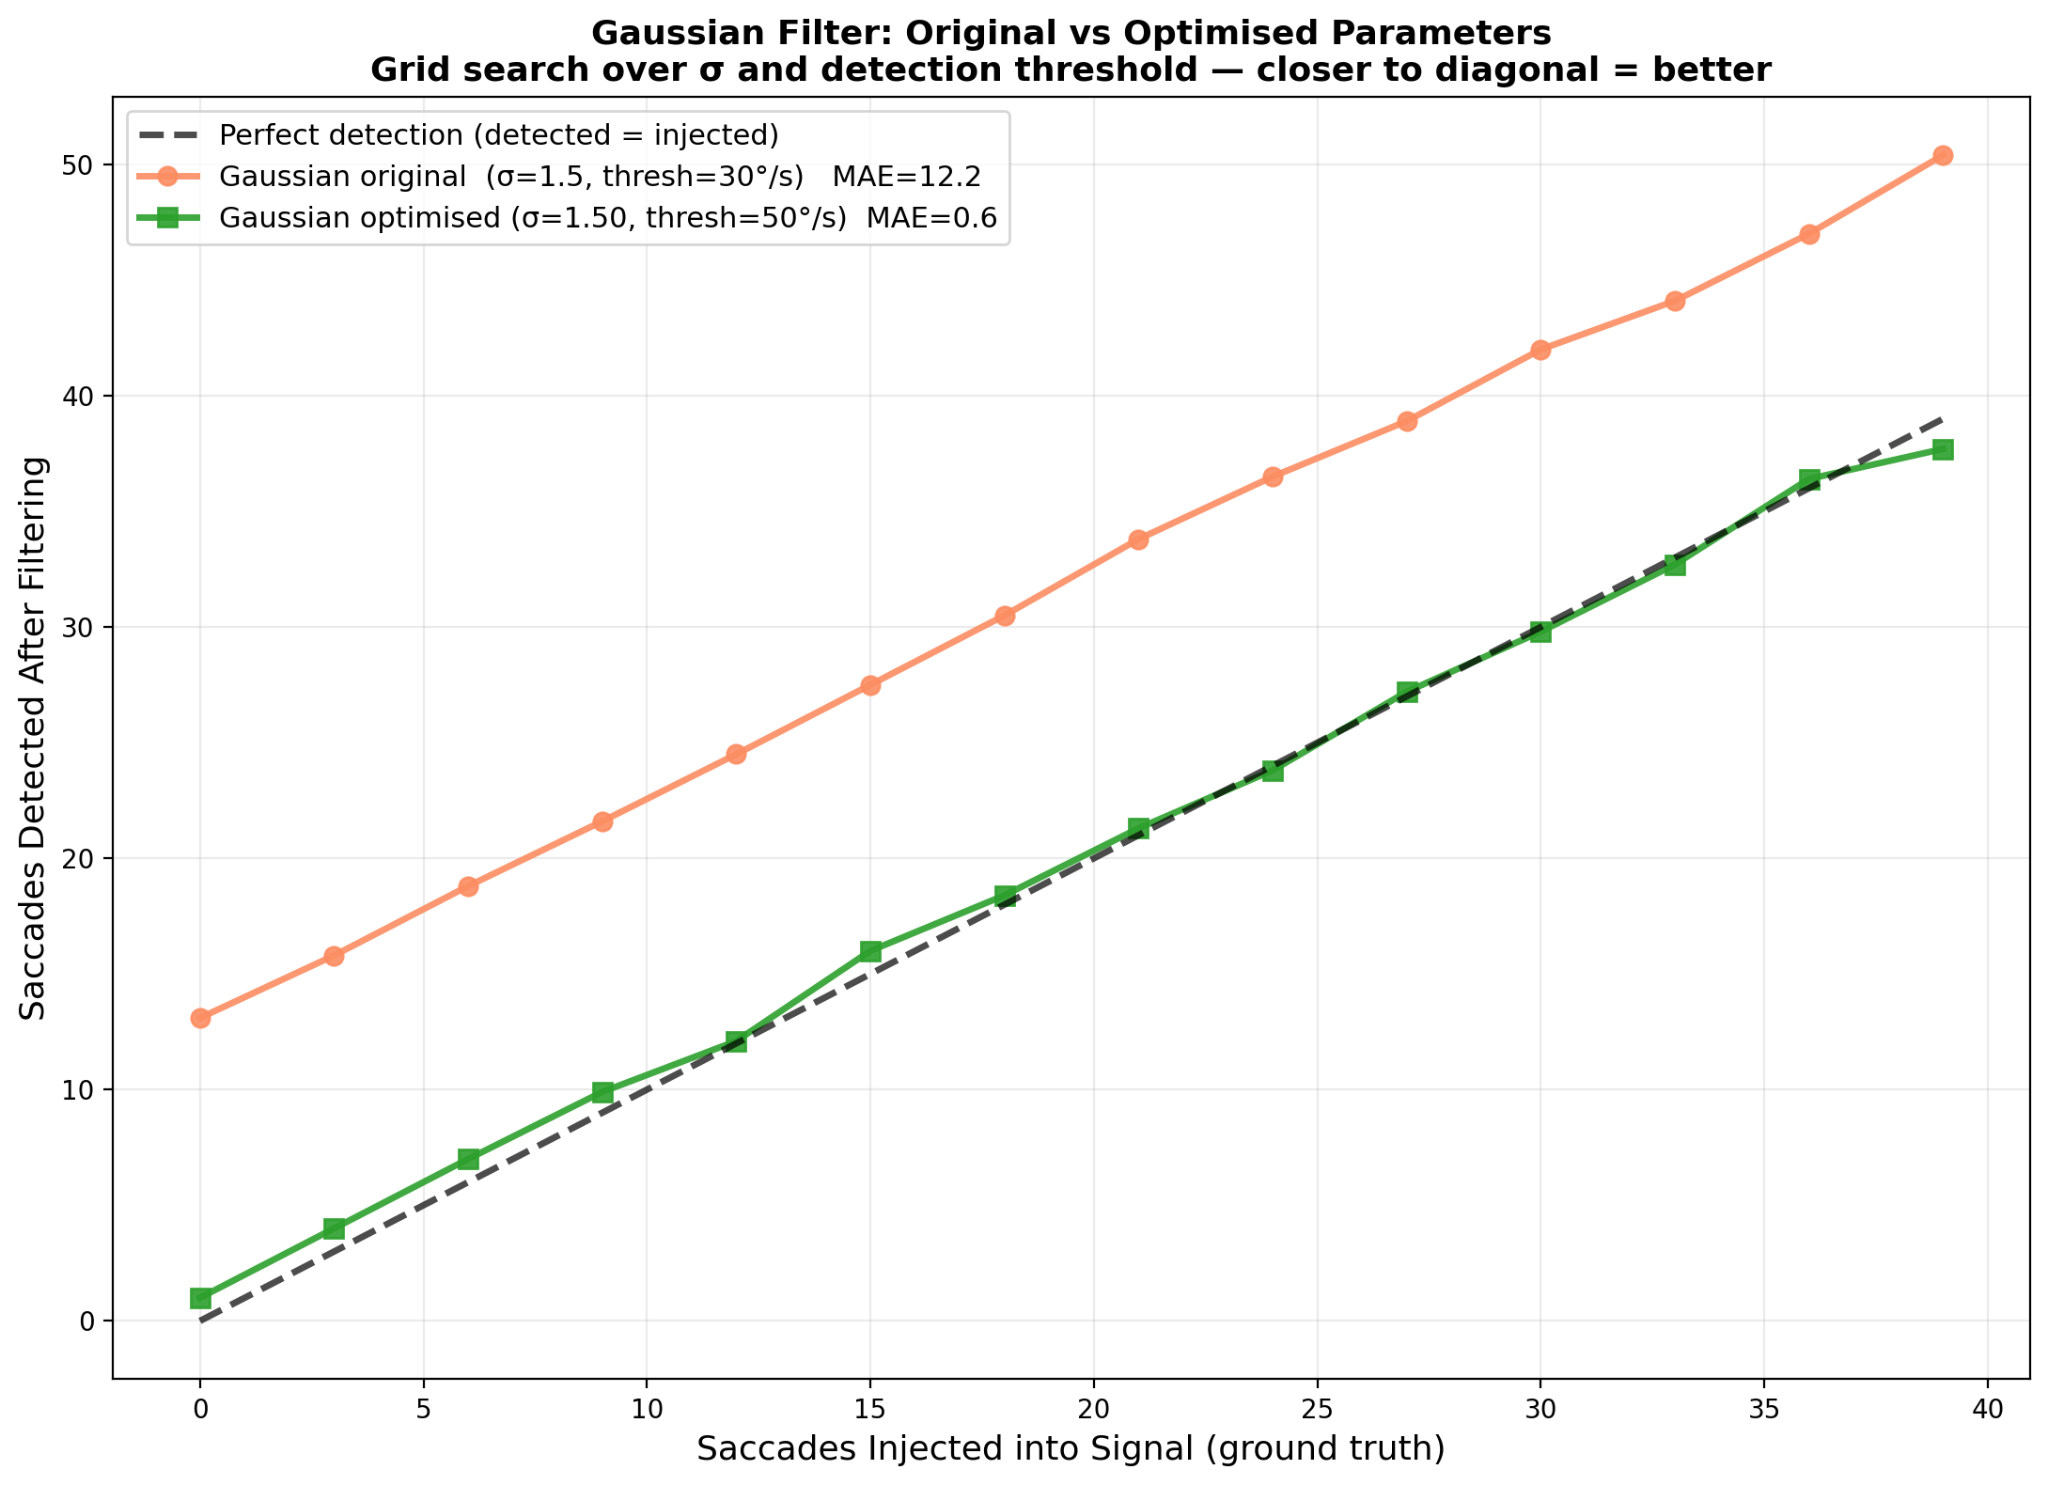
\includegraphics[width=\textwidth]{figures/gaussian_filter_optimisation}
    \caption{General filter performance comparison.}
    \label{fig:gaussian-optimisation}
\end{figure}

\Cref{fig:filter-comparison} shows that the Gaussian filter performs the best as it has the lowest error in saccade predictions. However, it still required optimisation, so a grid search was performed of the better Gaussian filters, achieving the filter in \Cref{fig:gaussian-optimisation}. The original unoptimised parameters were sigma~$=$~1.5 and threshold~$=$~30\,deg/s, giving MAE~$=$~12.2. Raising threshold to 50\,deg/s caught the real saccades, modelled as 120--240\,deg/s velocity peaks. These test results are evidence of the validity of this methodology.

\begin{figure}[htbp]
    \centering
    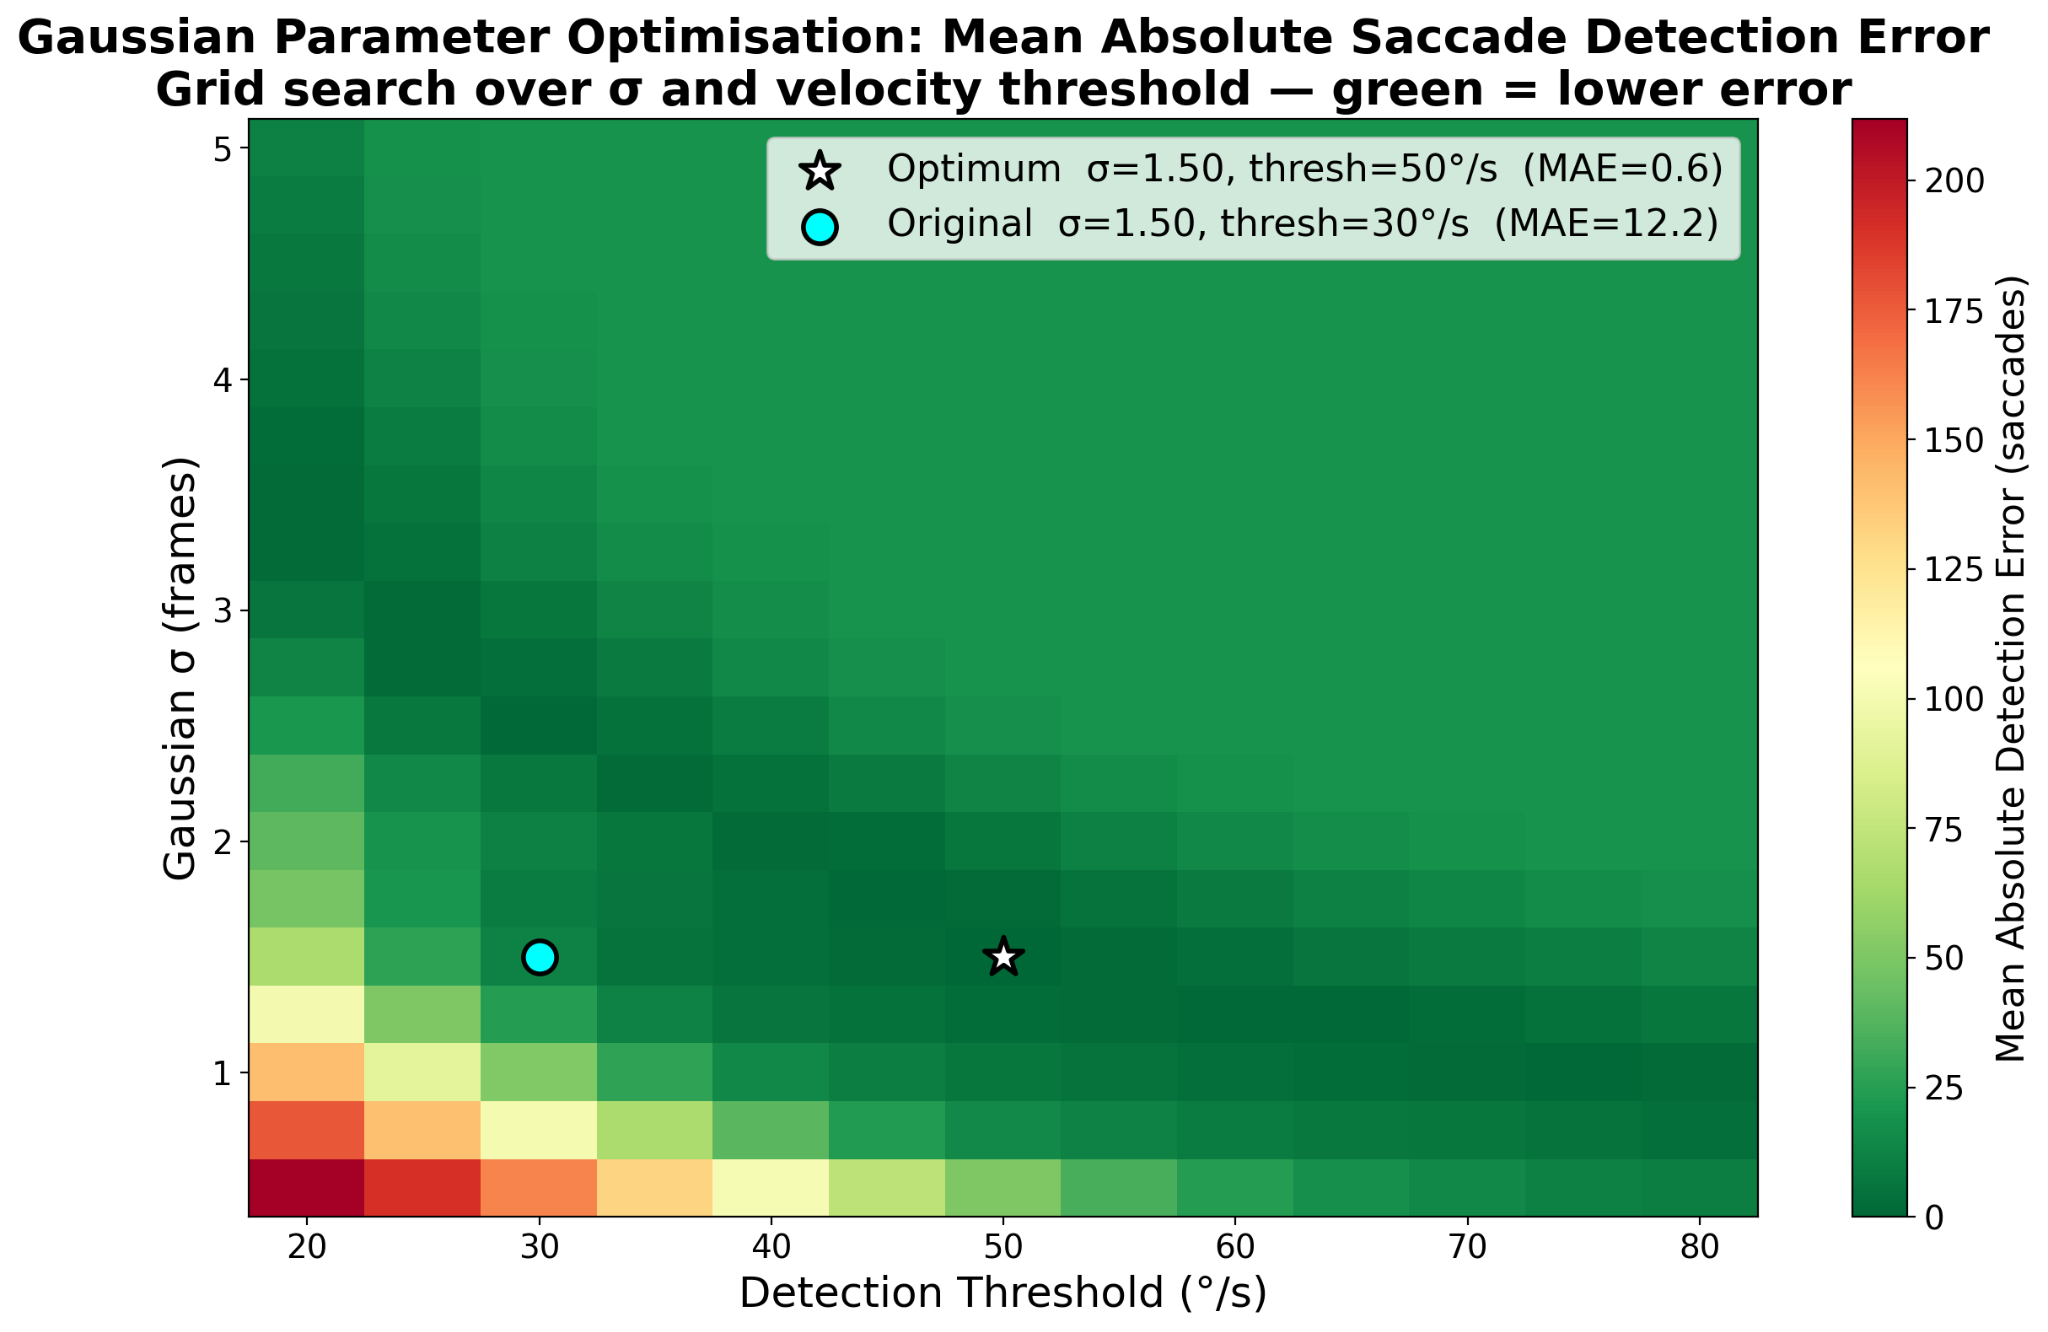
\includegraphics[width=\textwidth]{figures/optimal_gaussian_filter}
    \caption{Optimal Gaussian filter performance.}
    \label{fig:optimal-gaussian}
\end{figure}

\begin{figure}[htbp]
    \centering
    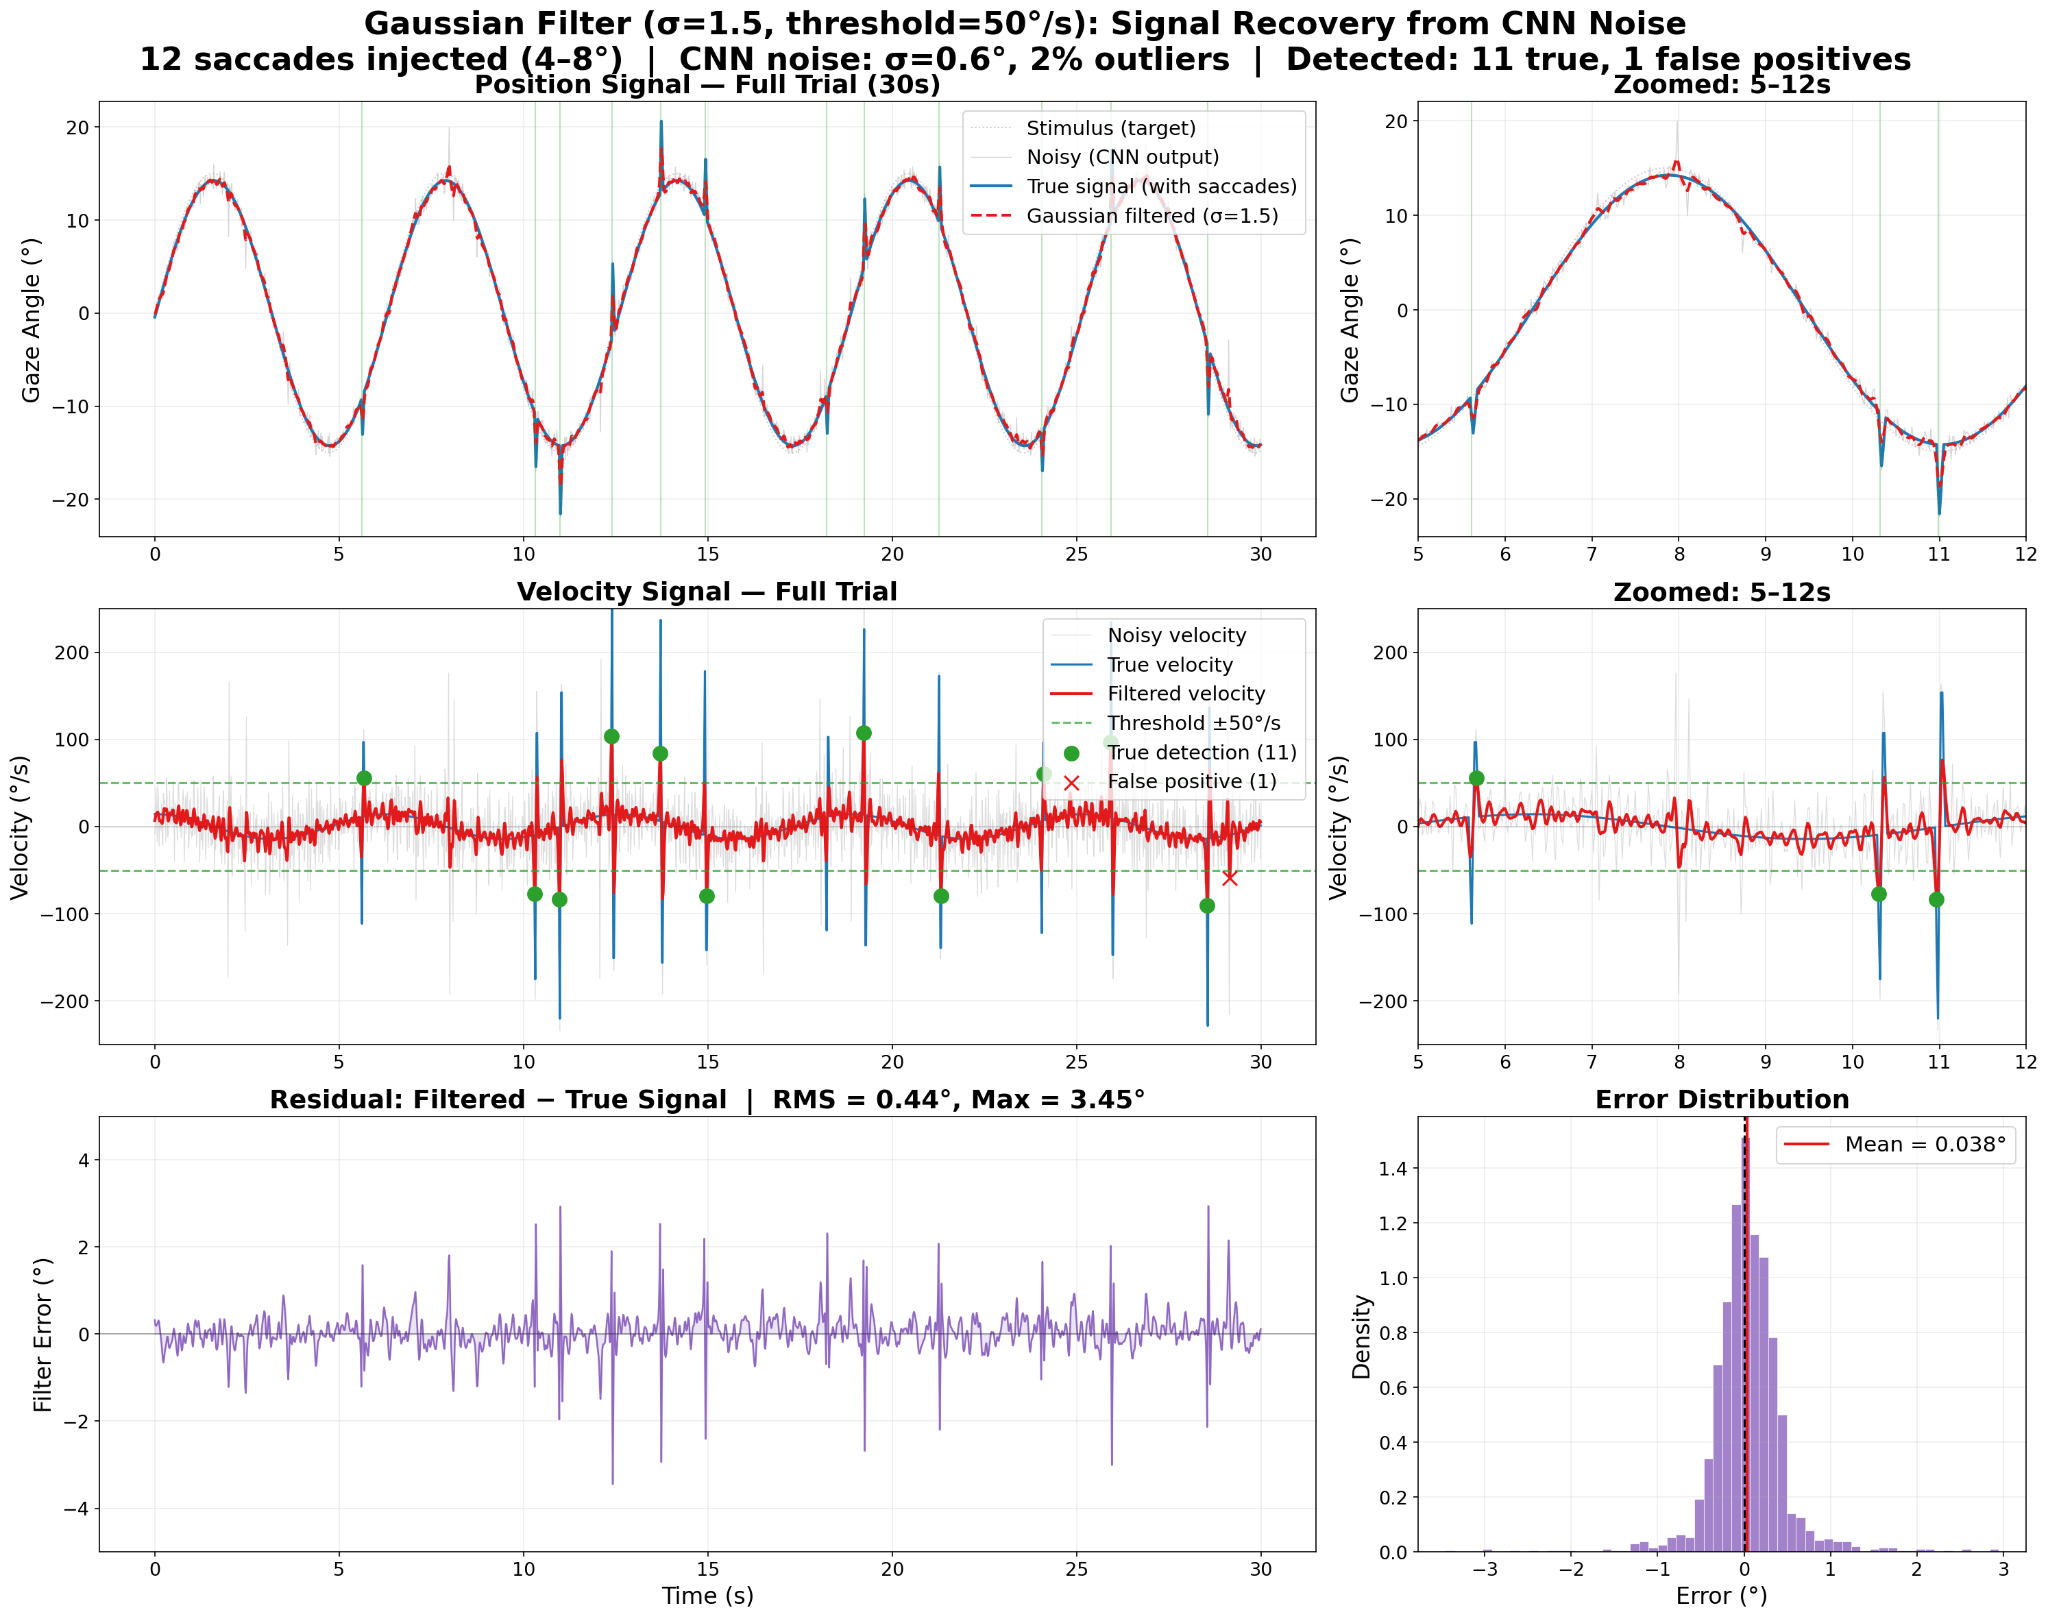
\includegraphics[width=\textwidth]{figures/filter_effects}
    \caption{Filter effects on a noisy signal.}
    \label{fig:filter-effects}
\end{figure}

\subsubsection*{Limitations and Future Improvements}

Saccades of 4--8 degrees of angular amplitude were injected for testing this filter, but there may be smaller ones that appear in future real headset data that would be harder to detect. This shows that the filter could be improved through using this same methodology further, iterating more in the future to provide the best filter for the end product. For now, this method has been proved and the parameters can be optimised later upon data collection, tuning noise and saccade amplitudes more appropriately. This is also the case for the glare, blurring, and IMU head shaking as further data collection is required to develop a more accurate threshold cutoff whilst using the same algorithms outlined in this section.

\section{Training Specific Technology}

The CNN used for understanding the gaze estimation was the MobileNetV2 model as it is explicitly designed for mobile and embedded vision workloads where inference must be fast and memory-efficient. Architectural features such as linear bottlenecks, inverted residual blocks, and depthwise separable convolutions reduce parameter count and the number of multiply-accumulate operations in comparison with heavier CNN alternatives, whilst still preserving useful representational capacity for strong feature understanding~\cite{sandler2018mobilenetv2}. This makes it a good fit for the Raspberry Pi~5 where the model is executed on the CPU whilst having to run camera capture, display update, logging, and Bluetooth/WiFi handling simultaneously. A plausible alternative would have been ResNet-18 as it is used widely for computer vision tasks, but it is computationally heavier than the MobileNetV2. Since this extra compute cost and power was not needed and we are optimising for faster and more efficient edge deployment, the MobileNetV2 was preferred over ResNet-18~\cite{he2016deep}.

The training process of the MobileNetV2 model was adapted to output the horizontal angle and achieve a low validation loss with strong generalisation. The pipeline was built and tested to show that the model structure is robust, so that when data is collected from the headset, the model can be trusted, leaving residual errors to be related to data needing further cleaning and augmentation. Methods are to be reused to automatically remove poor images from the dataset, using the confidence signals to remove poor data and prevent model corruption.

A custom regression head was applied as the MobileNetV2 classifier is designed for ImageNet classification rather than gaze-angle regression~\cite{sandler2018mobilenetv2}. The 1280-dimensional feature vector produced by the MobileNetV2 is then passed through the head which consists of Dropout ($p$~$=$~0.2), a linear reduction from 1280 to 512 dimensions, a ReLU activation, a second Dropout layer ($p$~$=$~0.2), and a final linear projection to the gaze-angle model.

ReLU and dropout layers are used to help prevent overfitting, for instance in subject-specific appearances~\cite{srivastava2014dropout}, supporting generalisation for new users and learning non-linear features of the data.

The backbone was fine-tuned from the start rather than freezing it as the domain gap between ImageNet photographs and the near-infrared eye images is large enough such that adaptation is needed beyond the final layers. This is consistent with the wider literature on transfer learning, showing that feature transferability decreases as the target tasks and input distribution diverge from the original pretraining domain~\cite{yosinski2014transferable}.

The loss function chosen was MSELoss which is optimal for 1D regression due to the continuous output with Gaussian noise~\cite{zhang2015appearance, krafka2016eye}. Both use MSE loss for gaze regression, showing this to be a conventional loss function for the task.

Adam~\cite{kingma2015adam} was selected as the optimiser with a learning rate of 0.001 for early testing, and SGD with momentum for once the hardware design has stabilised. Research found that SGD with momentum outperformed Adam in their eye tracking experiments~\cite{chugh2020eye}, achieving lower final validation loss despite the slower initial convergence. This result is also consistent with a broader finding in the optimisation literature where Adam will cause convergence to a sharp minima that generalises more poorly, whereas SGD's noisier gradient estimates usually have flatter minima with better generalisation~\cite{keskar2017large, wilson2017marginal}. Adam will be initially used, however, as the immediate need is using small amounts of collected data to reach stable and rapid convergence, where the model and preprocessing pipeline are still being iterated. A linear warmup schedule was also implemented that increased the learning rate from near-zero to the target value over the first 5 epochs. This was essential to do as the regression head is randomly initialised whilst the backbone carries the pretrained weights. Without the warmup, the large initial gradients from the head propagate backward and will destroy pretrained features before they have the opportunity to align with the new task. After the warmup, a ReduceLROnPlateau scheduler halves the learning rate if the validation loss stalls for 5 consecutive epochs.

\subsection{Architecture Validation on MPIIGaze}

To validate that these are sensible choices for a machine learning architecture independently of the headset hardware, the pipeline was evaluated on the MPIIGaze benchmark~\cite{zhang2015appearance}, a popular public dataset containing 213{,}659 normalised eye patches from 15 subjects with calibrated 3D gaze direction labels. Training was performed on NVIDIA A100 GPUs and a leave-one-person-out cross validation so that all the images from one subject are kept for testing whilst keeping the remaining 14 subjects for the training set. This is important as it ensures that the validation accuracy reflects true cross-subject generalisation. By showing a competitive accuracy on a known benchmark, this can show that errors in the headset model can be attributed to the headset domain-specific factors in its data collection such as camera resolution and viewing geometry, rather than issues with the model architecture and optimiser set out above. For robustness, both optimisers were used in this comparison.

\begin{table}[htbp]
    \centering
    \caption{15-fold LOPO cross-subject evaluation on MPIIGaze. Our pipeline matches published baselines with a substantially lighter backbone chosen for edge deployment on the Raspberry Pi.}
    \label{tab:mpiigaze-results}
    \begin{tabular}{lccc}
        \toprule
        \textbf{Method} & \textbf{Backbone} & \textbf{Test MAE (15-fold)} \\
        \midrule
        Zhang et al.~\cite{zhang2015appearance} & AlexNet-based & 6.3\textdegree{} \\
        Zhang et al.~\cite{zhang2017appearance} & ResNet-based & 4.80\textdegree{} \\
        Cheng et al.~\cite{cheng2018appearance} & Evaluation-guided asymmetric & 4.70\textdegree{} \\
        Ours (Adam) & MobileNetV2 (11.5\,MB) & 4.97\textdegree{} \\
        Ours (SGD) & MobileNetV2 (11.5\,MB) & 4.85\textdegree{} \\
        \bottomrule
    \end{tabular}
\end{table}

The pipeline achieved 4.97\textdegree{} (Adam) and 4.85\textdegree{} (SGD) mean MAE across the 15 folds, which is competitive with Cheng et al.\ (4.70\textdegree{}), Zhang et al.\ 2017 (4.80\textdegree{}), and 2015 (6.3\textdegree{}). This benchmark validates that the choices of training loop, loss function, and architecture are not the main limiting factor for gaze regression and that the residual error on the headset data is more strongly associated with domain-specific factors such as geometry, subject variance, and IR imagery. Therefore, future optimisations should consider data quality, labelling, and IR-specific augmentation whilst not excluding architecture-specific choices, but rather putting them as a secondary concern instead.

\section{Summary and Design Considerations of the Smooth Pursuit Trial}

The smooth pursuit software developed in this section has met the constraints identified including: GDPR, HIPAA, and CCPA compliance through image deletion; methodologies that are reusable and can be tuned further in the future (synthetic filter validation with MAE 0.6 saccades, architecture validation, basis thresholds); running on the Pi~5 with LiteRT achieving 2.68\,ms mean inference latency with the concurrent display and sensor workloads; developing a training pipeline that displays competitive metrics at 4.97\textdegree{} against literature values such as Cheng et al.\ (4.70\textdegree{}), Zhang et al.\ 2017 (4.80\textdegree{}), and 2015 (6.3\textdegree{}).

The main limitation throughout, however, is the lack of real headset data. This includes filter thresholds, quality gates, and IMU validity cutoffs which are provisional but can be rechosen using the same methodologies once the data becomes available. Architectural changes have not been completely struck off but are less of a concern in comparison with labelling quality, subject diversity, and IR-specific augmentation given the MPIIGaze results. The next steps should be headset data collection, thresholding retuning, and selecting a final optimiser.


\section{Pupil Width Estimation}
\label{sec:pupil-width}

This section describes the pipeline that converts raw eye images from the headset camera into \ab{plr} biomarker measurements. The pipeline must satisfy the following requirements, derived from the literature review  (\Cref{chapter:background}) and the headset hardware (\Cref{chapter:headset}):

\begin{itemize}
    \item \textbf{Precision.} Resolve the pupil diameter changes associated with \ab{plr} abnormalities in \ab{mtbi}, which manifest as differences of 15--20\% in constriction amplitude and 15--20\,ms in latency between concussed and healthy populations;~\cite{master2020pupillary, ciuffreda2017plr}).

    \item \textbf{Robustness.} Handle blinks (100--400\,ms of complete data loss) and other transient artefacts gracefully, detecting and discarding corrupted frames rather than propagating erroneous measurements.

    \item \textbf{Ease of use.} Operate without specialist training or equipment, producing measurements that are comparable across subjects.

    \item \textbf{Inference.} Complete processing within the 8.3\,ms per-frame budget imposed by the headset's 120\,fps capture rate on the Raspberry Pi~5.

\end{itemize}


\subsection{Pipeline Design}
\label{sec:pipeline}

\begin{figure}[htbp]
    \centering
    
\includegraphics[width=\textwidth]{pipeline_figure.pdf}
    \caption{Pupil width estimation pipeline overview. (a)~Preprocessing: raw eye images undergo contrast enhancement. (b)~Direct regression: a CNN predicts pupil diameter as a single scalar. (c)~Semantic segmentation: a CNN produces per-pixel class labels from which iris and pupil boundaries are extracted via ellipse fitting, yielding multiple outputs including confidence. (d)~Biomarker extraction: per-frame measurements are accumulated into a time series and fitted with a parametric PLR model to extract clinically relevant biomarkers.}
    \label{fig:pipeline}
\end{figure}

Two approaches dominate the recent literature for learning-based pupil measurement. In a \emph{regression} approach, a model predicts ellipse parameters directly from the raw image~\cite{kothari2021ellseg, jia2024condseg}. In a \emph{segmentation} approach, the model classifies each pixel into anatomical regions (pupil, iris, sclera, background) and an ellipse is fitted to the segmented boundary~\cite{chaudhary2019ritnet}.

We adopt segmentation. On \textbf{accuracy}, recent comparative work shows complementary strengths: regression achieves tighter ellipse centre localisation (1.12 vs 1.47\,px on OpenEDS), while segmentation produces higher-quality boundaries (97.4\% vs 94.6\% iris \ab{iou})~\cite{jia2024condseg, kothari2021ellseg}. Since our downstream task (tracking diameter changes over time) depends on boundary precision rather than absolute centre accuracy, segmentation is slightly better suited.

On \textbf{robustness}, segmentation produces a per-pixel probability map from which we derive per-frame confidence scores for automated quality gating: frames where the model is uncertain are downweighted or discarded before biomarker extraction, preventing corrupted measurements from propagating downstream. Regression provides no equivalent signal. On \textbf{interpretability}, the segmentation mask is directly inspectable: when the pipeline reports an anomalous \ab{plr} measurement, a user or developer can examine the mask to determine whether the anomaly reflects a genuine physiological response or a processing artefact.

The trade-off is \textbf{annotation cost} when adapting to new hardware. Pixel-level segmentation masks require minutes per image to produce, whereas regression labels (e.g.\ clicking two points on the pupil boundary) take seconds, making regression substantially cheaper to fine-tune on a new device. We offset this by training on existing datasets (OpenEDS; 12\,759 masks~\cite{garbin2019openeds}), applying domain-specific augmentation (\Cref{sec:domain-transfer}), and validating end-to-end using cheaply acquired regression-style diameter labels from our headset.

For a screening tool whose output may prompt referral to a medical professional, the robustness and interpretability advantages take priority over annotation cost: silent failures risk missed referrals, and the ability to audit predictions is essential for trust in the system's output. \Cref{tab:design-matrix} summarises the comparison.

\begin{table}[htbp]
\centering
\caption{Design comparison for pupil diameter extraction. \textbf{Bold} indicates the stronger approach for each criterion.}
\label{tab:design-matrix}
\begin{tabular}{l c c}
\toprule
\tableHCell{Criterion} & \tableHCell{Regression} & \tableHCell{Segmentation} \\
\midrule
Accuracy            & \multicolumn{2}{c}{Complementary (see text)} \\
Robustness          & No per-frame confidence & \textbf{Probability map} \\
Interpretability    & Opaque                  & \textbf{Inspect mask} \\
Annotation cost     & \textbf{Seconds/image}  & Minutes/image \\
Real-time inference & \multicolumn{2}{c}{Both feasible at 120\,fps} \\
\bottomrule
\end{tabular}
\end{table}

\subsection{Ablation}
\label{sec:ablation}

Within the segmentation pipeline, three factors must be configured: model architecture, loss function, and preprocessing. We ablate each on the OpenEDS benchmark to verify our choices. As shown in \Cref{tab:baseline-results}, performance is saturated across architecture and loss function choices; preprocessing is the only ablated factor that meaningfully affects accuracy.

All models are trained on OpenEDS~\cite{garbin2019openeds} (12\,759 annotated images, 152 participants) with the Adam optimiser (learning rate $10^{-3}$), ReduceLROnPlateau scheduling, for 50 epochs on an NVIDIA RTX A4000 (16\,GB). Due to compute constraints, we run three seeds for one configuration per architecture (RITnet + Dice, U-Net + CE) to characterise run-to-run variance, and single seeds for the remaining configurations.

\paragraph{Architecture.} Deployment on the headset's Raspberry Pi~5 imposes inference compute constraints (the 8.3\,ms per-frame budget at 120\,fps has not yet been verified on-device). We compare RITnet~\cite{chaudhary2019ritnet}, a lightweight DenseNet--U-Net hybrid (250K parameters, {<}1\,MB), against a standard U-Net (7.8M parameters, 29.6\,MB). As \Cref{tab:baseline-results} shows, both architectures achieve comparable pupil axis error (0.09 vs 0.13 $\pm$ 0.02\,px), but U-Net is 46\% slower and 30$\times$ larger.

\paragraph{Loss function.} Not all pixels matter equally for diameter estimation: accuracy depends on the pupil--iris boundary. We compare cross-entropy, generalised Dice (which addresses class imbalance by weighting each class inversely by area), CE + Dice, and a compound loss adding a boundary-aware term that upweights pixels near class edges~\cite{chaudhary2019ritnet}. The spread in axis error across all four is 0.04\,px (\Cref{tab:baseline-results}), comparable to the $\pm$0.03\,px seed-to-seed variance observed for Dice. Since the differences are within noise, we adopt the compound loss following the original RITnet paper: the boundary-aware term is theoretically motivated for our boundary-sensitive task, even though its empirical effect is small at this dataset scale.

\paragraph{Preprocessing.} Raw eye images exhibit low contrast between iris and pupil. We apply gamma correction ($\gamma = 0.8$, a nonlinear intensity mapping that brightens dark regions) and CLAHE (contrast-limited adaptive histogram equalisation; clip limit 1.5, tile grid $8 \times 8$), which enhances local contrast without amplifying noise globally. Removing both approximately triples axis error (0.10 to 0.32\,px), making preprocessing the only factor with a meaningful effect.

\begin{table}[htbp]
\centering
\caption{Configuration ablation on the OpenEDS test set. $^\dagger$Mean $\pm$ SD across 3 seeds. FPS measured on an NVIDIA RTX A4000.}
\label{tab:baseline-results}
\begin{tabular}{l l l r r r r}
\toprule
\tableHCell{Model} & \tableHCell{Loss} & \tableHCell{Preproc.} & \tableHCell{Pupil IoU (\%)} & \tableHCell{Axis err (px)} & \tableHCell{Size (MB)} & \tableHCell{FPS} \\
\midrule
RITnet & CE              & Yes & 98.76 & 0.10 & 1.07 & 160 \\
RITnet & Dice$^\dagger$  & Yes & 98.91 $\pm$ 0.02 & 0.12 $\pm$ 0.03 & 1.07 & 167 $\pm$ 10 \\
RITnet & CE + Dice       & Yes & 98.98 & 0.08 & 1.07 & 188 \\
\textbf{RITnet} & \textbf{Compound} & \textbf{Yes} & \textbf{98.93} & \textbf{0.09} & \textbf{1.07} & \textbf{148} \\
RITnet & CE              & No  & 97.82 & 0.32 & 1.07 & 226 \\
U-Net$^\dagger$  & CE    & Yes & 98.93 $\pm$ 0.10 & 0.13 $\pm$ 0.02 & 29.6 & 130 $\pm$ 3 \\
\bottomrule
\end{tabular}
\end{table}

We select RITnet with compound loss and gamma+CLAHE preprocessing as the deployment configuration (bold in \Cref{tab:baseline-results}).

\subsection{Domain Transfer}
\label{sec:domain-transfer}

\paragraph{Domain gap.} OpenEDS was collected using a research-grade eye tracker with near-infrared illumination, high-resolution optics, and controlled viewing geometry. The headset uses \todo{fill in camera details from electronics section} viewing through a beamsplitter under display-reflected visible light. \Cref{fig:domain-gap} illustrates the visual differences: the headset images are lower resolution, exhibit different contrast characteristics, and contain reflections from the beamsplitter optics.

\begin{figure}[htbp]
    \centering
    \begin{minipage}{0.35\textwidth}
        \centering
        
\includegraphics[width=\textwidth]{raw_eye_crop}
        \subcaption{OpenEDS (research eye tracker)}
    \end{minipage}
    \hfill
    \begin{minipage}{0.35\textwidth}
        \centering
        
\includegraphics[width=\textwidth]{headset_raw_cropped}
        \subcaption{Headset}
    \end{minipage}
    \caption{Domain gap between training data and deployment hardware. The images differ in resolution, contrast, illumination spectrum, and noise characteristics.}
    \label{fig:domain-gap}
\end{figure}

\paragraph{Augmentation strategy.} Annotating pixel-level segmentation masks for headset images is prohibitively labour-intensive (as discussed in \Cref{sec:pipeline}). Instead, we bridge the domain gap through data augmentation that simulates the headset imaging conditions during training. We evaluate two strategies of increasing specificity, with results in \Cref{tab:augmentation-results}.

\emph{Standard augmentation} applies geometric transforms (random horizontal flips, small rotations) and photometric perturbations (brightness, contrast, and Gaussian noise jitter) that improve generalisation across any target domain.

\emph{Domain-specific augmentation} adds transforms targeting the identified differences: sclera region brightening (simulating the different illumination balance), resolution downsampling (matching the headset's lower effective resolution), and blur (simulating slight defocus through the beamsplitter optics).

\begin{table}[htbp]
\centering
\caption{Effect of augmentation on OpenEDS test set performance and headset pupil detection rate. Augmentation reduces OpenEDS accuracy (as expected, since the training distribution is broadened) but dramatically improves headset generalisation.}
\label{tab:augmentation-results}
\begin{tabular}{l r r r}
\toprule
\tableHCell{Configuration} & \tableHCell{Pupil IoU (\%)} & \tableHCell{Axis err (px)} & \tableHCell{Headset detection (\%)} \\
\midrule
No augmentation (baseline)  & 98.93 & 0.09 & 22.1 \\
Standard augmentation       & 98.19 & 0.23 & \todo{--} \\
Domain-specific augmentation & 79.28 & 2.68 & 52.3 \\
Domain-specific + 112$\times$112 & 92.72 & 0.27 & \todo{--} \\
\bottomrule
\end{tabular}
\end{table}

The domain-specific augmentation at full OpenEDS resolution significantly degrades in-distribution performance (pupil \ab{iou} drops to 79.3\%) because the aggressive transforms push the training distribution far from the OpenEDS test set. Training at the headset's native resolution (112$\times$112) partially recovers OpenEDS performance (92.7\% \ab{iou}) while maintaining the domain adaptation benefit. On headset images, domain-specific augmentation increases pupil detection from 22\% to 52\%, with sensible diameter measurements (pupil/iris ratio $0.45 \pm 0.09$) where the baseline model produces largely invalid fits.

\paragraph{Headset validation.} \Cref{fig:headset-validation} shows segmentation overlays on headset-captured images for the baseline and domain-augmented models. The baseline model frequently fails to segment the pupil or produces fragmented predictions, whereas the domain-augmented model achieves coherent segmentation on the majority of frames where the pupil is visible. \todo{Add regression-label diameter comparison on ${\sim}100$ labelled headset frames.}

\begin{figure}[htbp]
    \centering
    \begin{minipage}{0.48\textwidth}
        \centering
        
\includegraphics[width=\textwidth]{headset_baseline_overlay}
        \subcaption{Baseline model (22\% detection)}
    \end{minipage}
    \hfill
    \begin{minipage}{0.48\textwidth}
        \centering
        
\includegraphics[width=\textwidth]{headset_domain_aug_overlay}
        \subcaption{Domain-augmented model (52\% detection)}
    \end{minipage}
    \caption{Segmentation results on headset-captured images. The baseline model (a) produces fragmented, mostly invalid predictions. Domain-specific augmentation (b) yields coherent pupil and iris segmentation on the majority of frames where the eye is visible.}
    \label{fig:headset-validation}
\end{figure}


\subsection{PLR Biomarker Extraction}
\label{sec:plr-extraction}

This subsection describes how per-frame segmentation masks are converted into clinically relevant \ab{plr} biomarkers. Each step is presented alongside the evidence that it works.

\paragraph{Diameter extraction.} Given a segmentation mask, we fit an ellipse to the largest pupil contour via least squares, yielding centre coordinates, major and minor axis diameters, and rotation angle. We report mean diameter (average of major and minor axes) for robustness to foreshortening from small head rotations within the headset.

The standard approach applies \texttt{argmax} to the segmentation logits before fitting, discarding the model's uncertainty. We improve on this with a probability-weighted fit: each pixel's contribution is weighted by its softmax probability of belonging to the pupil class, so uncertain boundary pixels have less influence than confident interior pixels. \todo{Report axis error improvement: hard vs soft fitting on OpenEDS test set.}

We normalise pupil diameter by the simultaneously measured iris diameter, producing a dimensionless pupil--iris ratio. Adult iris diameter varies by only ${\sim}3.4\%$ across individuals (11.8\,mm $\pm$ 0.4\,mm~\cite{boyle2021hvid}), so this ratio reflects true pupil size changes rather than geometric scaling, removing the need for per-subject calibration.

\paragraph{Signal cleaning.} The raw diameter time series contains frame-to-frame jitter, data gaps from blinks, and low-frequency pupil oscillations (hippus, 0.5--2\,Hz). Three steps clean the signal before biomarker extraction. \textbf{Blink detection:} frames where the pupil area drops below 50\% of the pre-stimulus baseline or where the segmentation confidence falls below a threshold are identified; short blinks are interpolated, while blinks during the constriction phase invalidate the trial. \textbf{Outlier rejection:} frames where the frame-to-frame diameter change exceeds 8\,mm/s (approximately mean + 2\,SD of healthy peak constriction velocity~\cite{bremner2012pupillometric}) are treated as segmentation failures and interpolated. \textbf{Savitzky--Golay filtering:} a local polynomial is fitted to each window for temporal smoothing~\cite{savitzky1964smoothing}. Unlike a Gaussian kernel, this preserves the sharp constriction onset that is critical for accurate peak velocity estimation.

\paragraph{Parametric curve fitting.} Rather than extracting biomarkers from local derivatives of the smoothed signal (which amplify noise), we fit a parametric model to the entire post-stimulus waveform~\cite{fan2011modeling}:
%
\begin{equation}
    d(t) = d_0 - A \left(1 - e^{-(t - t_{\mathrm{onset}})/\tau_c}\right) e^{-(t - t_{\mathrm{onset}})/\tau_d}
    \label{eq:plr-model}
\end{equation}
%
where $d_0$ is the baseline diameter, $A$ is the constriction amplitude, $t_{\mathrm{onset}}$ is the latency, $\tau_c$ is the constriction time constant, and $\tau_d$ is the dilation recovery time constant. The model is fitted via nonlinear least squares with physiologically informed bounds on each parameter. This acts as a physics-informed regulariser: every data point contributes to every parameter estimate, and the model rejects solutions that would correspond to impossible pupil dynamics. The fitted parameters directly yield the clinically relevant biomarkers identified in \Cref{chapter:background}: constriction latency ($t_{\mathrm{onset}}$), constriction amplitude ($A/d_0 \times 100\%$), peak constriction velocity ($\max |d'(t)|$, derivable analytically), and recovery time constant ($\tau_d$). \Cref{fig:plr-fitted} shows an example fit.

\begin{figure}[htbp]
    \centering
    
\includegraphics[width=0.85\textwidth]{plr_fitted_curve}
    \caption{Parametric curve fitting applied to a synthetic \ab{plr} waveform ($\sigma = 0.2$\,mm noise). The fitted model (red) yields constriction latency, amplitude, peak velocity, and recovery time constant. $R^2 = 0.965$.}
    \label{fig:plr-fitted}
\end{figure}

We validate robustness by generating 100 synthetic \ab{plr} waveforms at each of six noise levels ($\sigma = 0.05$ to $0.5$\,mm) and measuring parameter recovery against known ground truth (\Cref{fig:robustness-noise}). The parametric fit maintains $R^2 > 0.9$ up to $\sigma \approx 0.3$\,mm. Latency is the most robust parameter (error {<}0.04\,s across all noise levels), while amplitude and recovery time degrade at higher noise. In a separate blink injection experiment (3 to 10 consecutive frames zeroed at random post-stimulus positions), $R^2$ remains above 0.99 across all blink durations, confirming that the blink detection and interpolation pipeline effectively neutralises data dropout.

\begin{figure}[htbp]
    \centering
    
\includegraphics[width=\textwidth]{robustness_noise}
    \caption{\ab{plr} parameter recovery under increasing measurement noise (100 trials per condition). The parametric fit degrades gracefully; latency is the most robust parameter.}
    \label{fig:robustness-noise}
\end{figure}

\paragraph{Bilateral comparison.} The headset captures both eyes simultaneously, enabling bilateral \ab{plr} comparison. The relative afferent pupillary defect (RAPD), defined as the asymmetry in \ab{plr} parameters between eyes, is one of the most clinically significant pupillary findings in neurological assessment: even when absolute parameters fall within normal range, inter-eye asymmetry can indicate unilateral injury. We compute parameters independently for each eye and report the inter-eye difference for each biomarker.


\subsection{Limitations}
\label{sec:limitations}

The current pipeline has four principal limitations that define the scope for future work. First, the segmentation model is trained on OpenEDS; despite domain-specific augmentation, the gap to headset imagery may ultimately require fine-tuning on headset-specific annotated data to achieve clinical-grade accuracy. Second, the \ab{plr} extraction pipeline has been validated on synthetic waveforms with known ground truth; clinical validation with concussed and healthy participants is required to confirm that the parametric model captures the full range of pathological \ab{plr} responses observed in \ab{mtbi}. Third, the robustness experiments assume additive Gaussian noise, which may not fully characterise the headset's artefact profile (e.g.\ motion blur from head movement, specular reflections from the beamsplitter). Fourth, each frame is segmented independently; incorporating temporal context could improve frame-to-frame consistency but at the cost of increased model complexity and latency.


\section{Vergence Measurement}
\label{sec:vergence}

Vergence measurement reuses the gaze estimation pipeline described in \Cref{sec:gaze-estimation} to assess a different oculomotor biomarker: the \ab{npc}. During the vergence assessment, the headset display presents a target that moves progressively closer to the user along the depth axis. The system tracks the horizontal gaze angle of each eye independently; as long as the user can maintain binocular fixation, the two gaze vectors converge toward the target.

The \ab{npc} is identified as the target distance at which convergence breaks down, detected either by a sudden divergence in the estimated gaze angles (indicating that one eye has lost fixation) or by the user reporting diplopia. Because this measurement depends on the gaze estimation model's ability to track both eyes simultaneously and resolve small angular differences, the accuracy of the vergence assessment is directly limited by the gaze model's angular resolution. \todo{Detail the geometric conversion from gaze angles to convergence distance and report the achievable NPC precision.}

\chapter{Market Analysis}
\label{chapter:ent-market}

% Owner: Suleiman (market segmentation, stakeholders) + Victor (value proposition, PMF)

This chapter analyses the market opportunity for a headset-based oculomotor screening system for \ab{mtbi}, identifies the key stakeholders and users, and articulates the value proposition for each target segment.


\section{Market Segmentation}
\label{sec:ent-market-analysis}

\todo{Suleiman: Draft this section. Frame the product as a portable oculomotor screening headset for rapid concussion/mTBI assessment, aimed at settings where quick triage matters and access to specialist neurodiagnostics is limited.}

\subsection{Unmet Need in Concussion Assessment}

\todo{Why concussion assessment is a real unmet need — draw on the clinical need established in \Cref{chapter:introduction} but reframe for a commercial audience. Quantify the problem: incidence rates, costs of missed diagnosis, liability exposure for sports organisations.}

\subsection{Market Segmentation}

\todo{Define target markets in layers:
\begin{itemize}
    \item Primary beachhead: sports concussion assessment (elite and semi-professional rugby, football, contact sports)
    \item Adjacent clinical: emergency departments, urgent care, concussion clinics
    \item Future expansion: military, schools/universities, amateur sports organisations, remote/rural healthcare
\end{itemize}
Segment along four axes:
\begin{itemize}
    \item Use case: pitchside screening vs clinic/research use
    \item Buyer type: sports organisations, clinics, hospitals, research institutions
    \item Geography: UK first, then EU/US depending on regulatory logic
    \item Customer sophistication: expert clinical user vs non-technical operator
\end{itemize}
Avoid generic ``the healthcare market is big'' framing. Be specific about where the headset is valuable and realistically adoptable first.}

\subsection{Market Sizing}

\todo{Provide \ab{tam}/\ab{sam}/\ab{som} estimates with explicit assumptions. Include rough sales logic grounded in actual buyer counts (e.g.\ number of Premiership rugby clubs, number of UK EDs, number of university sports programmes), not abstract percentages of trillion-pound markets.}

\subsection{Adoption Dynamics}

\todo{Discuss likely early adopters vs later adopters. Why would research institutions and elite sports be first? What triggers broader adoption — regulatory endorsement, clinical evidence, insurance incentives, high-profile incidents?}


\section{Stakeholder Analysis and User Research}
\label{sec:ent-stakeholders}

\todo{Suleiman: Draft this section.}

\subsection{Stakeholder Map}

\todo{Identify all actors around the device:
\begin{itemize}
    \item Primary users: athlete/patient, sideline operator (physio, sports medic, coach)
    \item Clinical users: ED clinician, concussion specialist, researcher
    \item Decision-makers: team/club/school administrator, hospital procurement, \ab{nhs} buyer
    \item Influencers: parent/guardian (especially youth sport), insurer, regulator
\end{itemize}
Map influence vs interest for key stakeholders.}

\subsection{User Personas}

\todo{Produce 2--4 strong personas, e.g.:
\begin{enumerate}
    \item Sideline physiotherapist for a semi-professional rugby club
    \item ED clinician triaging mild head injuries in a busy department
    \item Concussion researcher collecting longitudinal pupilometry data
    \item School sports staff member with minimal technical training
\end{enumerate}
Each persona should include: role, goals, pain points, technical comfort, context of use, and what success looks like.}

\subsection{User Journeys}

\todo{Build user journeys covering:
\begin{enumerate}
    \item Pre-test: device setup, patient preparation, app connection
    \item Test execution: conducting assessment after suspected impact
    \item Result interpretation: receiving and understanding the result
    \item Post-test decision: repeat test, referral, return-to-play decision
    \item Data management: storing, uploading, reviewing historical data
\end{enumerate}
Connect tightly to product features: quick setup, non-technical operation, local inference, Bluetooth result to phone, Wi-Fi upload, motion quality flags, repeat-test recommendation.}


\section{Value Proposition}
\label{sec:ent-value-prop}

\todo{Victor: Draft this section.}

\subsection{Engineering Decisions as Buyer Value}

\todo{Translate design choices into buyer value:
\begin{itemize}
    \item Local inference on Pi $\rightarrow$ immediate result without cloud dependency
    \item Bluetooth result to phone $\rightarrow$ usable on sidelines without bulky equipment
    \item Wi-Fi deferred upload $\rightarrow$ research and model retraining value without slowing the test
    \item Fixed-focus optics and integrated display $\rightarrow$ simpler, more robust workflow
    \item IMU gating and quality flags $\rightarrow$ better trust in results
    \item Non-technical usability $\rightarrow$ broader adoption beyond specialist labs
\end{itemize}}

\subsection{Segment-Specific Value Propositions}

\todo{Write separate value propositions for each customer segment:
\begin{itemize}
    \item Sports medic: fast, portable, operator-friendly decision support
    \item Clinic: objective repeatable measure and digital record
    \item Researcher: standardised data capture and exportable dataset
    \item Organisation buyer: scalable screening workflow, reduced dependence on expert interpretation
\end{itemize}}


\section{Product-Market Fit}
\label{sec:ent-pmf}

\todo{Victor: Draft this section.}

\subsection{Problem-Solution Fit}

\todo{Test PMF by asking:
\begin{itemize}
    \item What painful problem does it solve better than the status quo?
    \item Is it urgent enough for buyers to act?
    \item Who pays, and through what budget line?
    \item Does the workflow fit actual practice, or does it require behaviour change?
\end{itemize}}

\chapter{Competitor Analysis}
\label{chapter:ent-competitive}

% Owner: Victor

This chapter maps the competitive landscape for concussion assessment tools, compares the headset against existing approaches, and analyses intellectual property considerations.


\section{Landscape of Concussion Assessment Approaches}
\label{sec:ent-competitive-landscape}

\todo{Victor: Map competitors into categories --- do not just list company names:
\begin{itemize}
    \item Traditional concussion screening: \ab{scat6}, CRT6, symptom checklists
    \item Digital cognitive assessment: ImPACT, CogSport, King-Devick
    \item Eye-tracking / pupilometry devices: NeurOptics NPi, EyeGuide Focus, BrightLamp Reflex
    \item Broader neurological monitoring: EEG headbands, blood biomarker kits
    \item Research systems not suitable for field deployment
\end{itemize}
Position the device against current concussion assessment approaches and explain that the system is not just ``another headset'' but a product with specific commercial logic: portable, objective, repeatable, less reliant on specialist expertise, supports both research and pitchside modes, functions offline/local-first.}


\section{Competitive Comparison}
\label{sec:ent-competitive-comparison}

\todo{Compare on key factors:
\begin{itemize}
    \item Portability and field suitability
    \item Objectivity of measurement
    \item Operator skill required
    \item Speed of assessment
    \item Cost and accessibility
    \item Regulatory maturity
    \item Real-time result delivery
\end{itemize}
Present as a comparison table where possible.}


\section{Intellectual Property}
\label{sec:ent-ip}

\todo{Address freedom to operate. Discuss:
\begin{itemize}
    \item What is hard to patent (known subsystems: cameras, Pi, beamsplitters)
    \item What may be patentable: multimodal workflow integration, signal processing pipeline, headset-specific optical arrangement for simultaneous stimulus delivery and eye imaging, quality-gated decision logic
    \item Whether the real moat is patents, data, clinical validation, or partnerships
\end{itemize}
Be realistic: strongest defensibility likely comes from evidence base, multimodal dataset, workflow integration, and validated deployment, not hardware novelty.}

\chapter{Roadmap}
\label{chapter:ent-adoption-roadmap}

% Owner: Suleiman

This chapter develops the adoption roadmap for the headset-based mTBI screening system, identifying the sequence of stakeholder groups that should be targeted and why. The phases are evaluated using evidence from stakeholder interviews, power dynamics within different settings and frameworks to create an evidence-based map of why this sequence was chosen. The downstream go-to-market execution plan is then developed in \Cref{chapter:ent-gtm}.


\section{Technology Adoption Curve}
\label{sec:ent-roadmap-adoption-curve}

\begin{figure}[htbp]
    \centering
    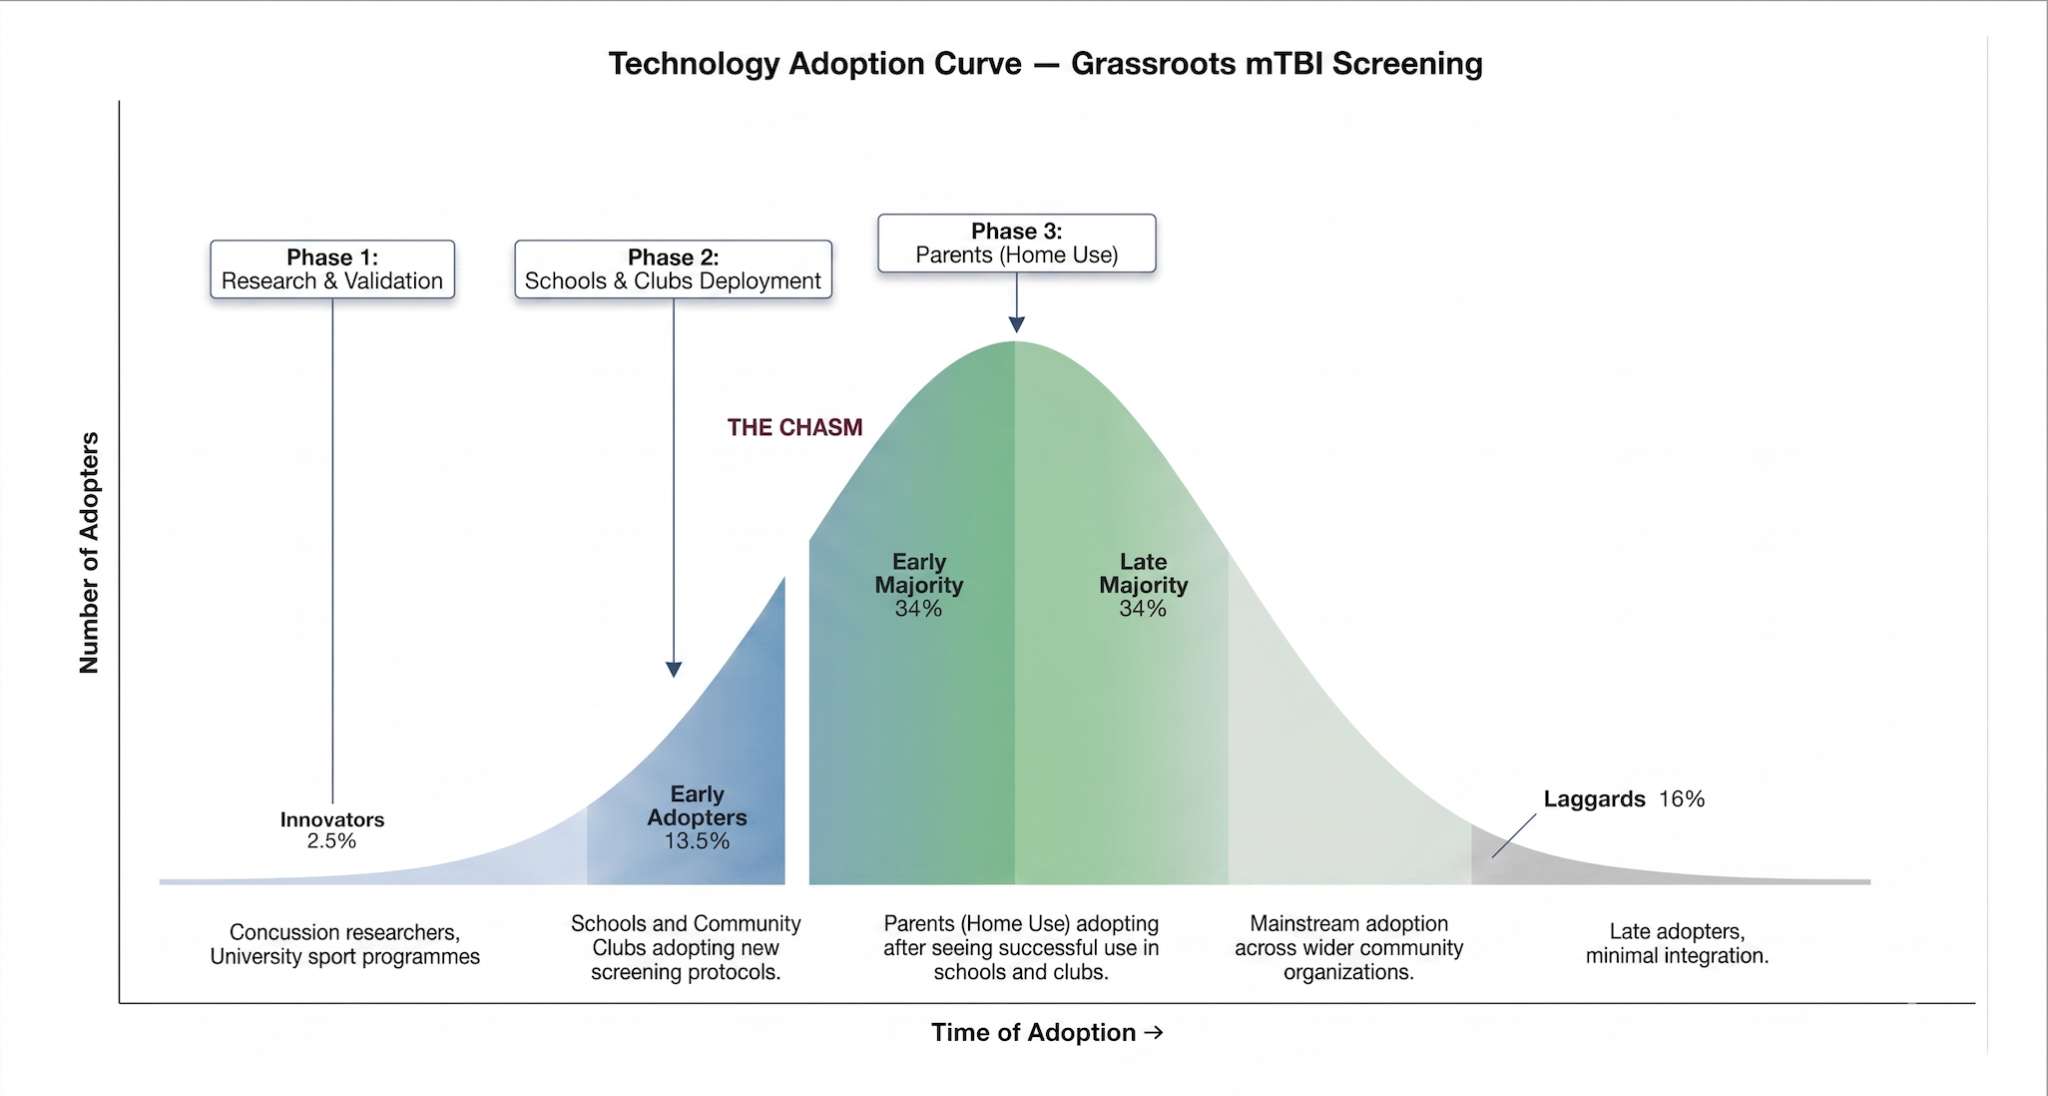
\includegraphics[width=0.85\textwidth]{figures/eem/technology_adoption_curve}
    \caption{Technology adoption curve for grassroots mTBI screening.}
    \label{fig:ent-technology-adoption}
\end{figure}

Using Rogers' diffusion of innovations~\cite{rogers2003diffusion}, Phase 1 consists of innovators which are concussion researchers in this context. They have the frameworks to test unvalidated tools (CUREC) and are motivated by publishing papers and making breakthroughs in emerging fields whilst not requiring a fully functioning product to start testing it. This is advantageous as the product is yet to be regulatory approved here (\Cref{chapter:ent-regulatory}) and under the lean startup build, measure, learn framework~\cite{ries2011lean} this would allow for iteration sequences, converging towards the best product that can be deployed to the market and producing a published validation paper producing strong evidence for acceptance of the stakeholders in Phase 2.

Phase 2 are the early adopters, where schools and youth clubs are targeted. These stakeholders such as the PE teachers, headmasters and coaches will adopt research evidence and institutional endorsement as they see the potential in the product, not because of popularity. This was supported by an interview with a headmaster, a high power, high interest stakeholder in these settings as per the figures below, who said they would ``use it every single time once validated to be safe and useful by experts''. This is typical early adopter behaviour.

The chasm identified by Moore~\cite{moore1991chasm} follows these phases after which we reach Phase 3 with the early majority of the mass market of parents who would want more evidence of a functioning product before using it such as prior use in school, exhibiting early majority behaviour. These last two phases are cumulative; Phase 2 generates institutional validation to assist Phase 3 as well as verifying strategies to expand within the community of schools and clubs which continue through Phase 3 to the mass market of schools, clubs and parents at home.

To justify these claims and sequence of phases to appropriately match the different groups to the characteristics of the phases, these statements were grounded in strong evidence. Appropriate methods covered to support this included user interviews, the ACCORD framework[176], and stakeholder dynamics.

\FloatBarrier
\begin{figure}[!htbp]
    \centering
    \begin{minipage}{0.32\textwidth}
        \centering
        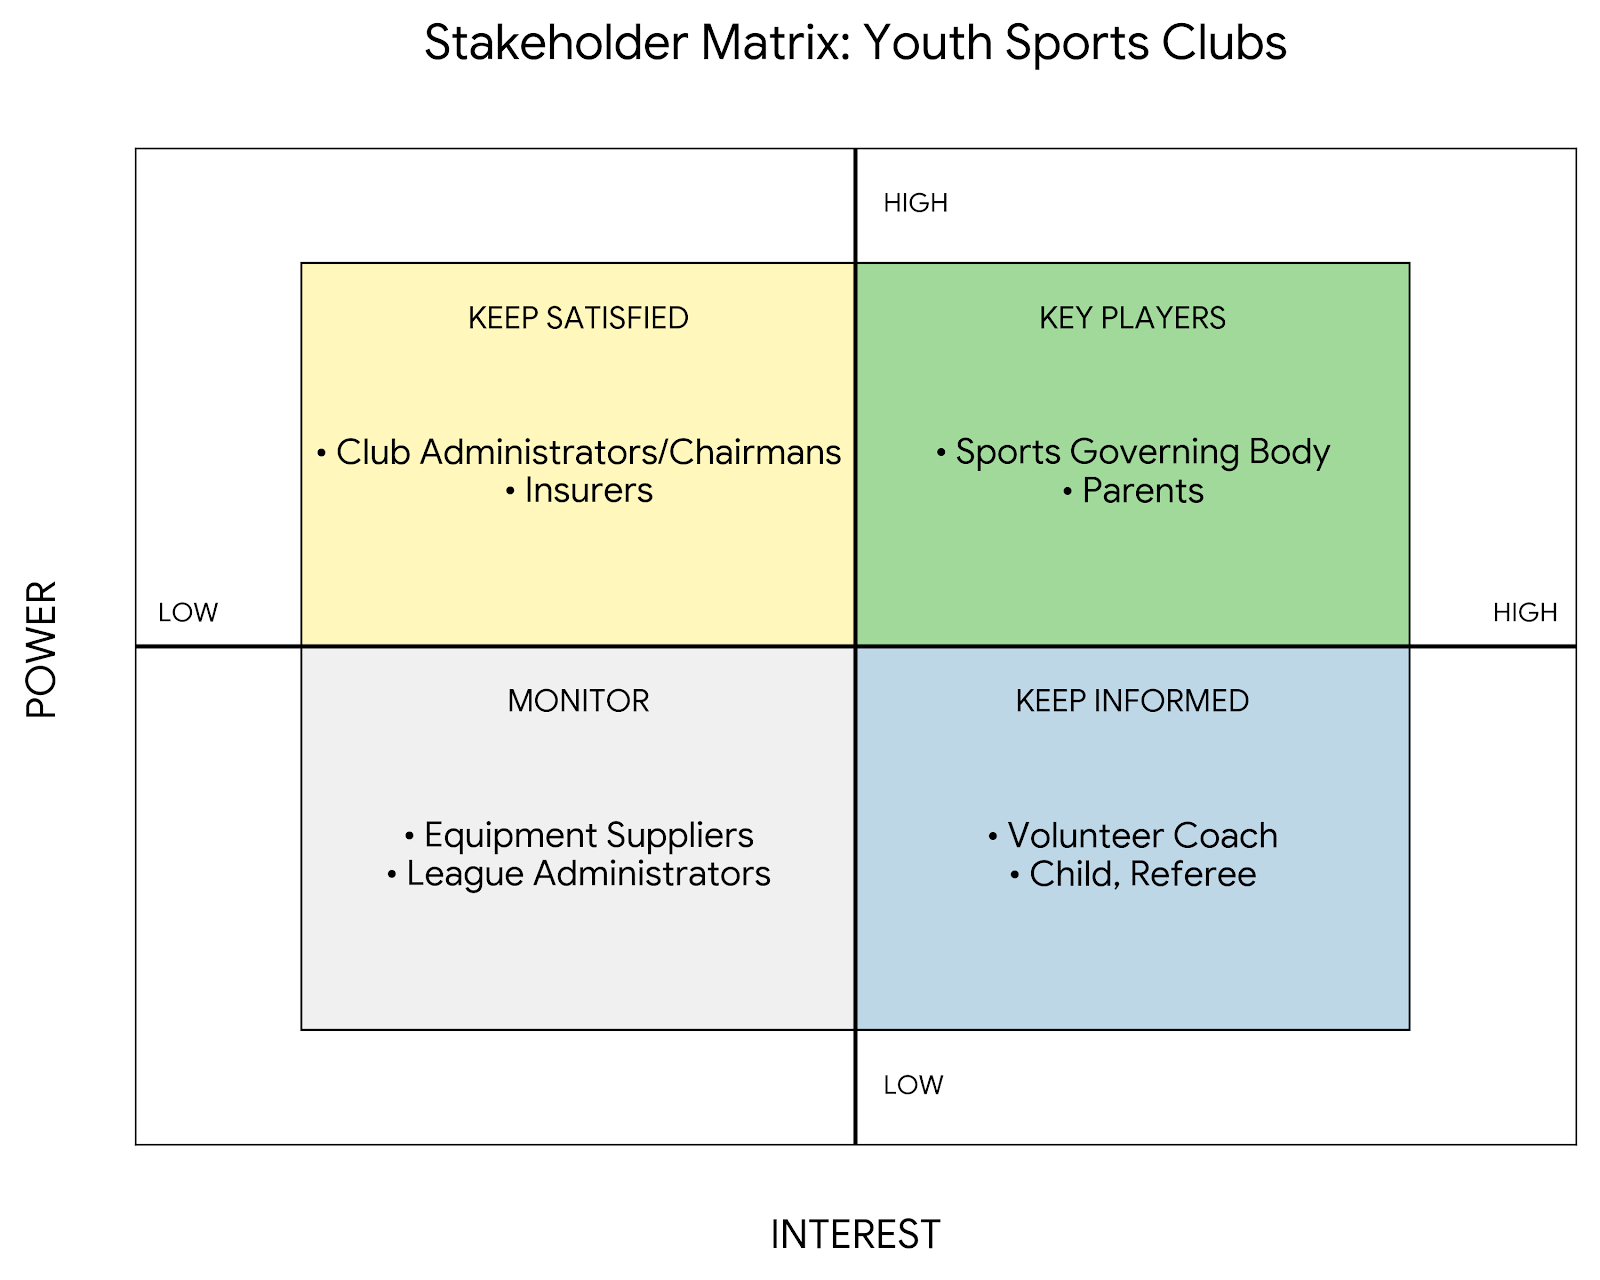
\includegraphics[width=\textwidth]{figures/eem/stakeholder_matrix_youth_sports_clubs}
        \subcaption{Youth sports clubs}
        \label{fig:ent-stakeholder-youth-clubs}
    \end{minipage}\hfill
    \begin{minipage}{0.32\textwidth}
        \centering
        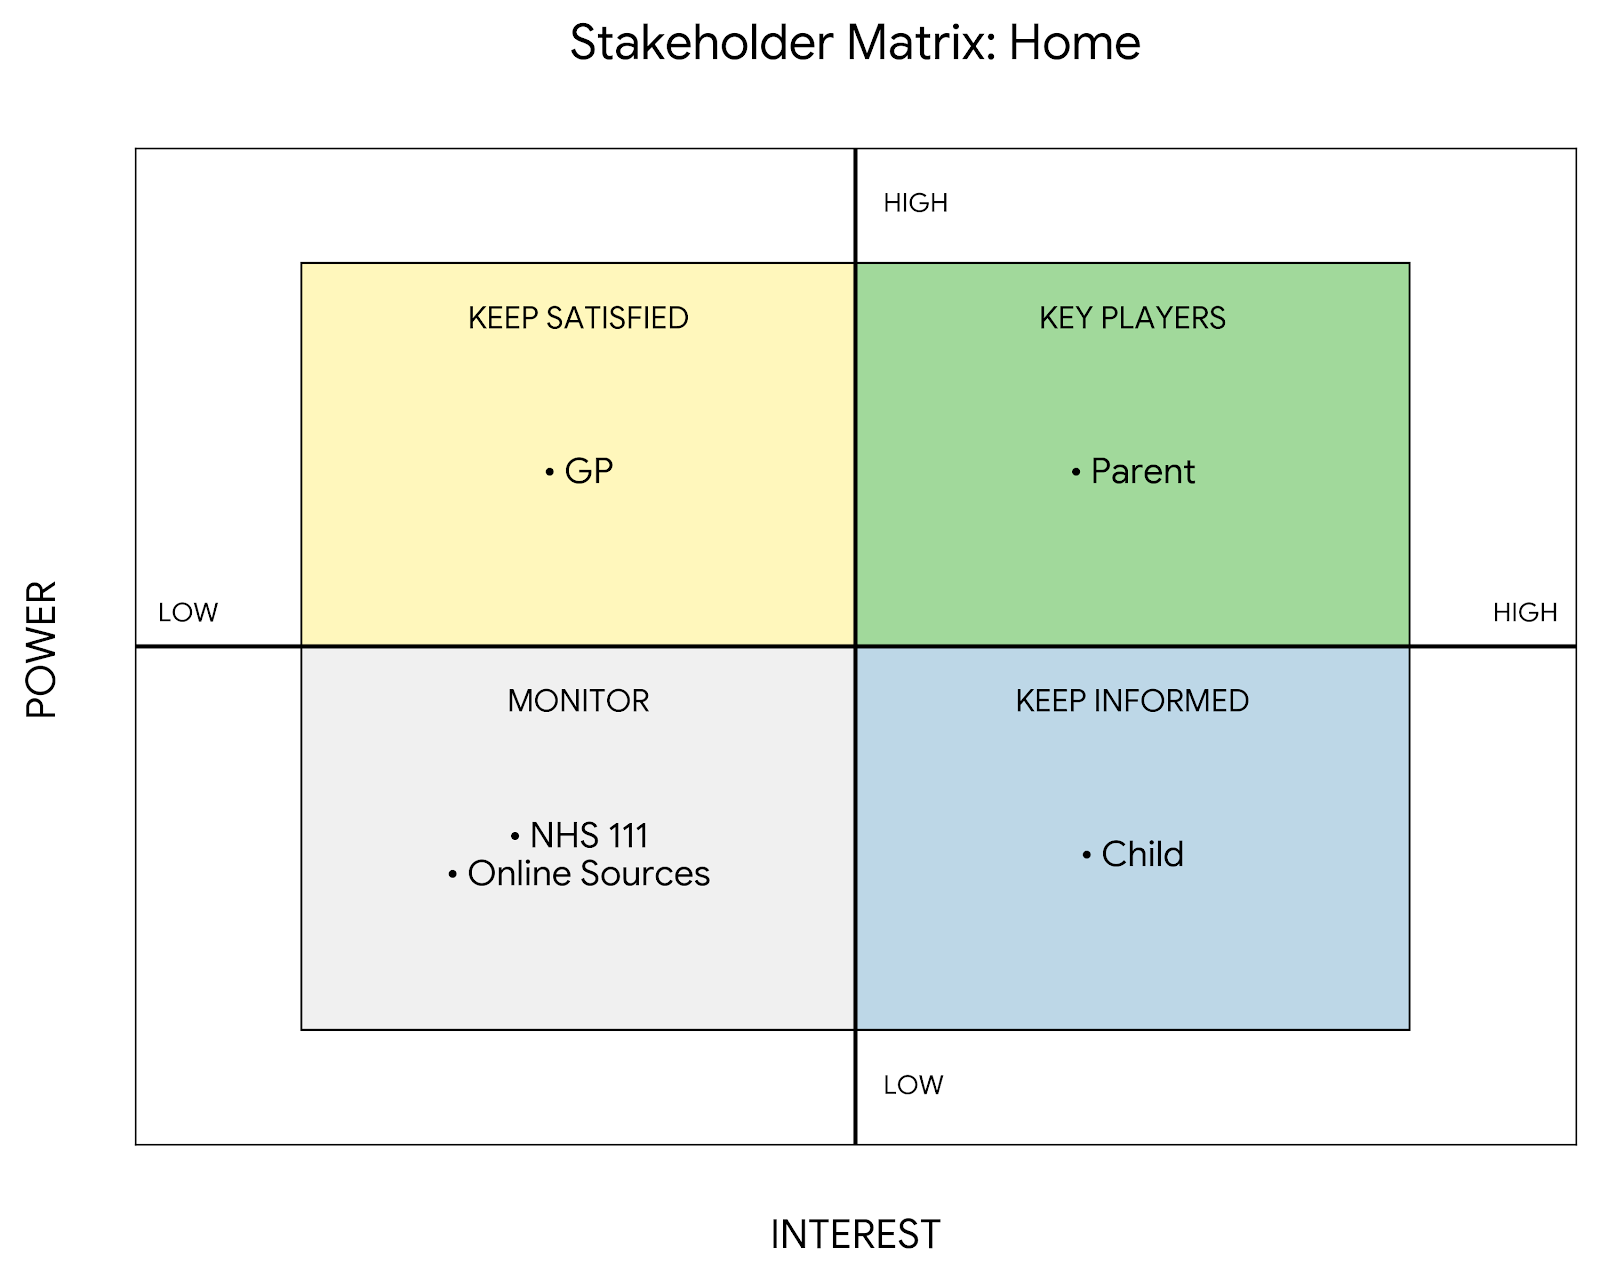
\includegraphics[width=\textwidth]{figures/eem/stakeholder_matrix_home}
        \subcaption{Users at home}
        \label{fig:ent-stakeholder-home}
    \end{minipage}\hfill
    \begin{minipage}{0.32\textwidth}
        \centering
        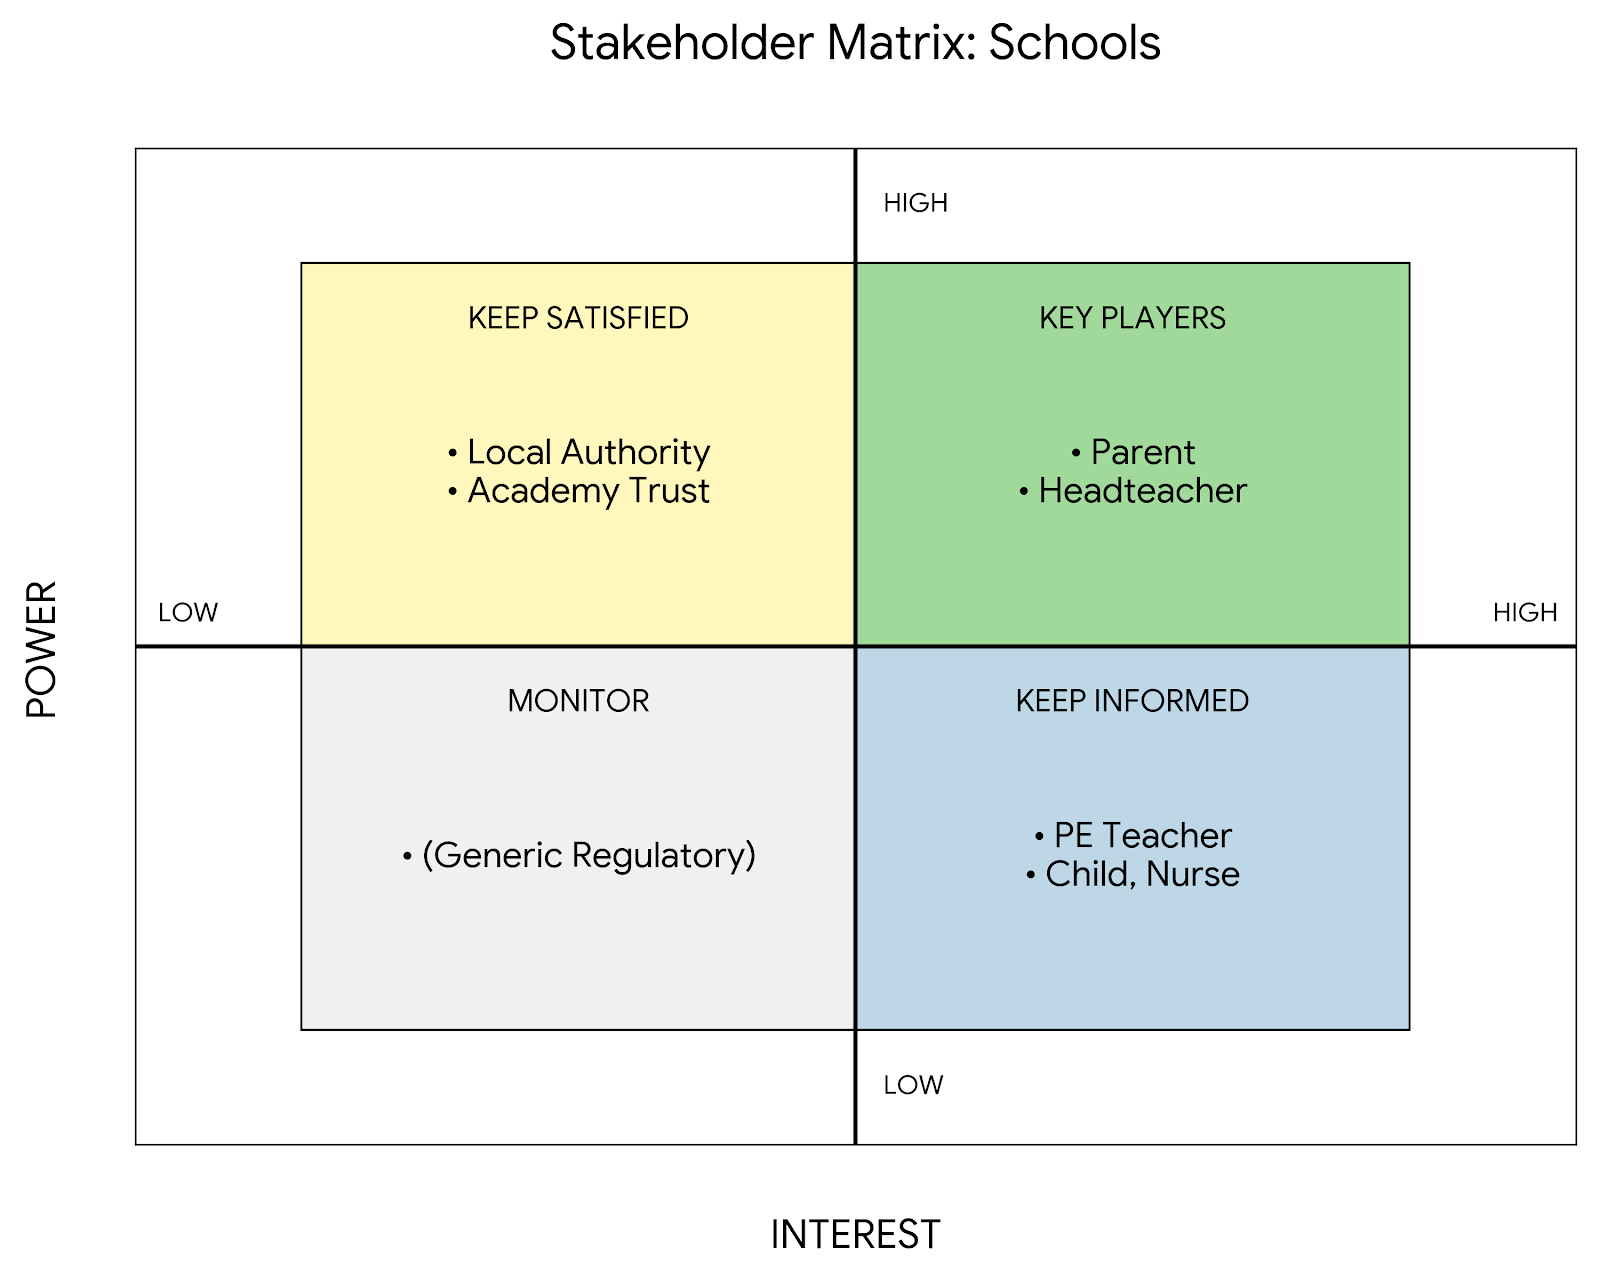
\includegraphics[width=\textwidth]{figures/eem/stakeholder_matrix_schools}
        \subcaption{Users at school}
        \label{fig:ent-stakeholder-schools}
    \end{minipage}
    \caption{Power-interest grids across the three target deployment settings.}
    \label{fig:ent-stakeholder-grids}
\end{figure}
\FloatBarrier

The power interest grids across the different settings of deployment show that parents are persistently high power, high interest stakeholders, driving user interviews to understand what must be in place for them to adopt the product. Statements of parents included ``if 100 schools are using it, I would feel confident'' and ``not something untested'', verifying that there should be sales and validation from schools and clubs before targeting large volume sales to parents.

Additionally, applying the ACCORD framework helps understand how quickly an innovation can be adopted. Analysing this in comparison with and without the prior phase to understand which order is more fruitful relative to each other yielded the following results.

\paragraph{Advantages.} In either case the tool would be better than non-trained coaches and parents by providing an objective measurement that is easy to use. No relative claim could be made here.

\paragraph{Compatibility.} The social compatibility would be relatively larger with Phase 2 than without as using a tool that is used by schools would make the parents feel like they are being a ``good, involved parent'' as verified in a user interview.

\paragraph{Complexity.} For both cases the tool is easy to use, providing low complexity with a simple app interface developed in \Cref{chapter:software}. No relative claim could be made here either.

\paragraph{Observability.} With Phase 2, the observability would be high due to the social proof of the tool being used on pitches and recognisable coaches motivating parents that are watching on the sidelines or hear by word of mouth as per the user interview. Without Phase 2, there would be less evidence for this as they would be beginning at the same time, the amount of observations of the tool's benefit would be lower. This reasoned a relative adoption benefit of having Phase 2 before Phase 3.

\paragraph{Risk.} With Phase 2, the perceived risk would be lower as per the user interview. Without Phase 2 the evidence would not be there to support the parents' worry, pushing favour towards Phase 2.

\paragraph{Divisibility.} With Phase 2, the product would already readily exist among certain schools and clubs at a larger scale than without phase 2, leading to easier trial use, pushing towards relative favour of Phase 2.


\section{Conclusions and Limitations}
\label{sec:ent-roadmap-conclusions}

Through applying the appropriate frameworks, a strong argument was made for pushing forward this adoption sequence. However, the limited number of user interviews, and perhaps a more complicated story of the risk-averse behaviour exhibited by this population, can equally justify selling to parents as soon as there has been regulatory approval. Such an argument could claim if they are risk-averse~\cite{stone2013selfother,dore2014parental}, they would adopt it immediately to help the child.

\chapter{Regulatory Landscape}
\label{chapter:ent-regulatory}

% Owner: Eesh

This chapter examines the regulatory environment for the headset-based \ab{mtbi} screening device, covering product classification, geographic entry pathway selection, claims language, and data privacy obligations. Unlike conventional B2B or B2C technology products, MedTech products require significant emphasis on regulatory constraints due to the intricacy and global complexity of approval processes~\cite{frontiers2024medtechregulation}. These constraints arise in two stages: (i) ethics approvals and health-data governance during data collection and device development, and (ii) intended-use claims, conformity assessments and clinical evidence requirements during commercialisation~\cite{hra_medical_devices,gov_uk_software_apps}. This chapter aims to optimise the product's survival probability by selecting jurisdictions which minimise regulatory friction and align with the chosen GTM strategy in \Cref{chapter:ent-gtm}.


\section{Product Classification}
\label{sec:ent-classification}

The intended purpose of the device must be defined explicitly, as the regulatory pathway changes significantly depending on its product classification~\cite{gov_uk_samd}. Three positionings are available, each with different burden/claim trade-offs:
\begin{itemize}
    \item \textbf{Wellness tool} -- lowest regulatory burden, but limits the claims that can be made about clinical utility and excludes use within the workflow of medical professionals.
    \item \textbf{Decision-support / screening aid} -- moderate burden, permitting the device to support but not replace clinical decision-making.
    \item \textbf{Class IIa medical device} -- highest burden where formal screening or diagnostic claims are made.
\end{itemize}
The headset-based \ab{mtbi} detection product is positioned as a \emph{supporting assessment / screening aid} rather than a \emph{concussion diagnosis device}. This deliberately reduces the regulatory burden during commercialisation, while preserving the clinical credibility that distinguishes the product from a pure consumer wellness device. The implications of this choice for the language used in marketing and product documentation are discussed further in \Cref{sec:ent-claims}.


\section{Phase 1 Jurisdiction: UK}
\label{sec:ent-regulatory-uk}

The UK was selected as the ideal location for Phase 1 of the GTM strategy. Australia, Singapore, the US, and Denmark were also considered, but the UK was chosen for two main reasons. First, the UK has established research governance structures for data collection from \ab{nhs}-affiliated concussion clinics and educational institutions. Second, this choice is operationally realistic for an Oxford-based team with warm access to local research and clinical networks. Although the UK is not the lowest-friction market from an administrative standpoint, it offers the greatest strategic alignment for Phase 1.

\subsection{NHS Research Approval Pathway}

The route by which data can be collected from concussion clinics is the NHS Research Approval Pathway. Our study should be framed as a \emph{formally governed medical-device research study} rather than a \emph{prototype test} in order to support later commercialisation. The Health Research Authority (HRA) states that ethical approval is required for a clinical investigation undertaken by a commercial company to demonstrate the safety and performance of a non-UKCA/CE marked medical device~\cite{hra_medical_devices}. To achieve approval from the Research Ethics Committee (REC), our study must be submitted through the Integrated Research Application System (IRAS). The REC will then evaluate the study on patient involvement, scientific and social value, and confidentiality before allowing it to start. This process allows NeuroScreen to demonstrate its ethics-oriented approach throughout product iteration.

As the parallel data collection from a university sports facility supports the same device investigation, the HRA requires a non-NHS/HSC Site Assessment Form to be provided within the IRAS application~\cite{hra_uk_governance}. This allows the suitability of the non-NHS site to be evaluated by the same REC, which is advantageous for Phase 1: both data-collection venues are assessed and approved through a single regulatory pathway, reducing the administrative cost associated with the process.

\subsection{Data Protection in Phase 1}

Phase 1 places a substantial emphasis on data protection. The collected dataset will contain raw eye video, derived physiological features and baseline information for each user. The Information Commissioner's Office (ICO), which upholds the General Data Protection Regulation (GDPR) in the UK, classifies such health data as \emph{Special Category Data}~\cite{ico_special_category}. This requires submission of a Data Protection Impact Assessment (DPIA) demonstrating a lawful basis for processing under Article 6(1)(e), which permits processing necessary in the public interest~\cite{gdpr_art6}, and Article 9(2)(j), which permits processing for scientific research purposes~\cite{gdpr_art9}. These obligations align with NeuroScreen's emphasis on strict data-collection pipelines, enabling transparency around data retention timelines, access controls and remote storage processes.

Adhering to this rigorous data-collection pathway allows NeuroScreen to generate a clinically credible and internationally reusable evidence package. This reduces the adoption risk associated with Phase 2 by cultivating credibility amongst professional clubs and medical professionals, and supports Phase 3, where the device is offered to non-medical end users (parents) who demand higher reliability assurances.


\section{Phase 2 Jurisdiction: EU}
\label{sec:ent-regulatory-eu}

The EU was chosen for Phase 2. While the UK and Australia are attractive markets for early traction, the EU offers the most scalable first commercial launch due to access to multiple member states through a single regulatory pathway. This aligns with the company's accessibility goals while operating as a lean startup, reducing the per-market regulatory cost of commercialisation.

\subsection{CE Marking and Classification}

To sell the device in the 32 member states of the EU, a Conformit\'{e} Europ\'{e}enne (CE) Mark is required. The first step of the commercialisation pathway is submitting an intended-use statement to the Medical Device Coordination Group (MDCG). EU guidance on medical-device classification states that the intended use of a device is decisive in its classification and qualification~\cite{eu_mdcg_classification}. Rule 11 within the MDR framework classifies \emph{software intended to provide information used to take decisions with diagnostic or therapeutic purposes} as a Class IIa device~\cite{eu_mdcg_classification}. CE-mark approval for a Class IIa device typically takes between 6--9 months~\cite{medenvoy_ce_timeline}. To maximise NeuroScreen's survival chances, the headset's intended-use statement will state that it \emph{supports \ab{mtbi} assessments} rather than diagnosing them, minimising both the approval timeline and the downstream evidence burden (consistent with \Cref{sec:ent-claims}).

\subsection{Conformity Assessment}

Following classification, a conformity assessment is required. A limitation of the EU route is that the pathway requires more than a functioning prototype: the European Commission requires manufacturers to maintain a quality management system and risk management system as set out in Article 9 of the MDR, alongside a clinical evaluation and post-market clinical follow-up~\cite{eu_md_manufacturers}. Although these requirements are demanding, they force NeuroScreen to build robust internal structures at seed stage, future-proofing the business while simultaneously meeting regulatory needs. Detailed quality control, risk assessment, and lifecycle and environmental impact assessment workflows would be developed as part of the Phase 2 entry plan.


\section{Claims Language}
\label{sec:ent-claims}

\todo{This is critical. Discuss what the product can and cannot claim:
\begin{itemize}
    \item ``Supports assessment'' --- lower regulatory burden
    \item ``Screening aid'' --- moderate
    \item ``Decision support'' --- moderate
    \item ``Diagnoses concussion'' --- not permissible without full clinical trial evidence and Class IIa/IIb clearance
\end{itemize}
Recommend claims language for each phase of the roadmap in \Cref{sec:ent-mvp}.}


\section{Prototype vs Commercial Device}
\label{sec:ent-prototype-vs-commercial}

\todo{Clarify what is permissible for a student/research prototype vs what changes for a commercial device. The current prototype operates under university research ethics approval --- what additional requirements apply for commercial deployment?}

\chapter{Business Plan}
\label{chapter:ent-business}

This chapter defines the commercial structure of the venture: how revenue is generated, what the first deployable product includes, how the supply chain scales from prototype to production, and how operations are structured. The analysis draws on the hardware and software design presented in \Cref{chapter:headset,chapter:software} and the market context established in \Cref{chapter:ent-market}. Financial projections derived from these assumptions are presented in \Cref{chapter:ent-financial}.


\section{Revenue Model and Pricing}
\label{sec:ent-revenue}

\subsection{Revenue Model}

\todo{Define candidate revenue models and justify the preferred approach. Consider:
\begin{itemize}
    \item Hardware sale + software subscription
    \item Hardware lease (institutional buyers)
    \item Research licence tier
    \item Per-test pricing (and why it may be inappropriate for the primary use case)
\end{itemize}
State the recommended model and why.}

\subsection{Pricing Strategy}

\todo{Define pricing for hardware, software tiers, and lease options. Justify against:
\begin{itemize}
    \item Competitor pricing (clinical pupillometers, sideline assessment equipment)
    \item Target customer willingness to pay (from market analysis)
    \item Required margins to fund regulatory and development costs
\end{itemize}}


\section{MVP Definition and Roadmap}
\label{sec:ent-mvp}

\subsection{Current Prototype vs MVP}

\todo{Distinguish between the 3YP prototype and a deployable MVP. What does the MVP include? What is explicitly deferred?}

\subsection{Development Roadmap}

\todo{Define phased development:
\begin{itemize}
    \item Phase 1: Research validation
    \item Phase 2: Pitchside deployment
    \item Phase 3: Clinical and institutional scale
\end{itemize}
Key milestones, timeline, and what de-risks each phase.}


\section{Supply Chain}
\label{sec:ent-supply-chain}

\subsection{Bill of Materials}

\todo{BOM breakdown by subsystem at prototype, low-volume, and medium-volume scales. Include a table.}

\subsection{Manufacturing Strategy}

\todo{How manufacturing evolves with volume:
\begin{itemize}
    \item Prototype (in-house, 3D printed)
    \item Low volume (batch SLS, outsourced PCB assembly)
    \item Medium volume (injection moulding, contract manufacturer)
\end{itemize}
Discuss turnkey vs tolling tradeoffs.}

\subsection{Quality Control and Calibration}

\todo{Optical alignment as the primary quality-critical operation. Mechanical precision vs software calibration approach.}

\subsection{Sourcing Risks}

\todo{Key supply chain risks: compute module availability, camera module continuity, optical component sourcing.}


\section{Unit Economics}
\label{sec:ent-unit-economics}

\todo{Bridge between supply chain and financial projections:
\begin{itemize}
    \item Hardware cost vs retail price, gross margin
    \item Assembly, testing, packaging, fulfilment costs
    \item Contribution margin per unit
    \item Subscription revenue per customer (blended across tiers)
    \item Lifetime value per customer
\end{itemize}}


\section{Operations}
\label{sec:ent-operations}

\todo{Operational structure of the venture:
\begin{itemize}
    \item Org structure and headcount plan (by phase/year)
    \item Key roles and estimated compensation
    \item Office/facilities requirements
    \item Insurance (product liability, professional indemnity, clinical trial insurance)
    \item Field operations: maintenance, cleaning protocols, battery management, software updates, warranty and support
\end{itemize}}

\chapter{Go-to-Market Strategy}
\label{chapter:ent-gtm}

% Owner: Suleiman

This chapter defines the strategy for bringing the headset to its first customers, covering beachhead selection, pilot design, sales channels, and partnership development.


\section{Beachhead Market Selection}
\label{sec:ent-beachhead}

\todo{Suleiman: Justify the choice of first customer segment. A sensible sequence:
\begin{enumerate}
    \item Research / validation deployments with university sports medicine groups
    \item Elite and semi-professional sport (rugby, football)
    \item Broader clinical pathways (ED, concussion clinics) once evidence and regulatory progress mature
\end{enumerate}
Why does the beachhead matter for credibility and evidence generation?}


\section{Pilot Strategy}
\label{sec:ent-pilots}

\todo{Define:
\begin{itemize}
    \item Number and type of pilot sites
    \item Success criteria for pilots
    \item Timeline from pilot to commercial deployment
    \item What the pilot proves to future customers
\end{itemize}}


\section{Sales and Distribution}
\label{sec:ent-sales}

\todo{Discuss:
\begin{itemize}
    \item Direct sales vs distributor model
    \item Partnerships with sports organisations, clinics, universities
    \item Role of the phone app as part of the adoption funnel
    \item Evidence-led adoption: published validation data as sales collateral
\end{itemize}}


\section{Partnership Strategy}
\label{sec:ent-partnerships}

\todo{Identify key partnership types:
\begin{itemize}
    \item Clinical research partners for evidence generation
    \item Sports governing bodies for credibility and access
    \item Medical device distributors for scale
    \item \ab{kol}s in sports medicine and concussion research
\end{itemize}}

\chapter{Financial Plan}
\label{chapter:ent-financial}

This chapter presents the financial projections for the venture. Unit economics and operational cost assumptions draw on the supply chain analysis in \Cref{sec:ent-supply-chain} and the adoption scenarios in \Cref{chapter:ent-gtm}. The first four sections cover the core financial model; the funding strategy in \Cref{sec:ent-funding} addresses how the venture is capitalised through to breakeven.


\section{Key Assumptions}
\label{sec:ent-assumptions}

\todo{Present a clear assumptions table covering:
\begin{itemize}
    \item Unit cost and retail price (by volume tier)
    \item Subscription pricing and churn rate
    \item Customer acquisition timeline (from GTM chapter)
    \item Headcount and compensation schedule (from operations)
    \item Regulatory and development cost estimates
    \item Working capital assumptions (inventory, receivables, payables)
\end{itemize}
This table should be the single source of truth for all subsequent projections. The reader should be able to change an assumption and understand how it flows through.}


\section{Profit and Loss Projection}
\label{sec:ent-pnl}

\todo{5-year P\&L with:
\begin{itemize}
    \item Revenue breakdown (hardware, subscriptions, research licences)
    \item Cost of goods sold
    \item Gross profit and margin
    \item Operating expenses by category (R\&D, sales, regulatory, G\&A)
    \item EBITDA
\end{itemize}
Include a table and a chart showing revenue vs costs over time. Explain the path to breakeven.}


\section{Cash Flow Projection}
\label{sec:ent-cash-flow}

\todo{5-year cashflow with:
\begin{itemize}
    \item Operating cashflow (EBITDA adjusted for working capital changes)
    \item Investing cashflow (capex, tooling, software capitalisation)
    \item Financing cashflow (equity injections)
    \item Closing cash balance
\end{itemize}
Highlight the minimum cash point and what it implies for funding requirements.}


\section{Sensitivity Analysis}
\label{sec:ent-sensitivity}

\todo{Stress-test key assumptions:
\begin{itemize}
    \item Base case, conservative, and optimistic scenarios
    \item What happens if adoption is 50\% slower?
    \item What happens if BOM costs are 30\% higher?
    \item What happens if regulatory takes an extra year?
    \item Tornado chart or similar showing which assumptions have the largest impact on breakeven timing
\end{itemize}
This section demonstrates rigour and shows which variables the business is most sensitive to.}


\section{Funding and Investment Strategy}
\label{sec:ent-funding}

\todo{Eesh: Draft this section.}

\subsection{Development Cost Estimate}

\todo{Estimate total development costs across phases.}

\subsection{Funding Requirements}

\todo{Total capital required to reach breakeven, timing and staging of funding rounds.}

\subsection{Funding Sources}

\todo{Evaluate candidate funding sources: grants, angel, VC, non-dilutive.}

\subsection{Investor Proposition}

\todo{Summarise the investment case: return profile, value inflection points, comparable exits.}

\chapter{Funding and Investment Strategy}
\label{chapter:ent-funding}

% Owner: Eesh

This chapter addresses how the capital requirement identified in \Cref{chapter:ent-financial} is bridged: how much to raise, with what staging, and from which sources. The plan is built directly on the unfunded cash trajectory of \Cref{sec:ent-cash-flow} and on the venture-stage classification of MedTech start-ups in the literature.


\section{Funding Envelope}
\label{sec:ent-fund-req}

The unfunded cash-flow projection of \Cref{sec:ent-cash-flow} reaches a peak trough of approximately \pounds3.71\,m in Y6, which sets the minimum funding required before the business is self-financing. Although NeuroScreen is a hardware MedTech venture, a sector notorious for high capex requirements~\cite{meridian_medtech_capex}, the model does not show a primarily capex-driven capital need. Manufacturing capex totals only \pounds112\,k across the seven-year horizon (approximately 3\% of the unfunded trough), reflecting the partial-turnkey arrangement of \Cref{sec:ent-mfg-sourcing}. The binding capital requirement is instead negative operating cash flow from payroll, regulatory work, software and hardware iteration, and early commercial execution: average operating burn between Y1 and Y6 is approximately \pounds605\,k/yr, peaking at \pounds838\,k in Y4 and \pounds858\,k in Y5 (\Cref{sec:ent-projection}).

A prudent but capital-efficient funding envelope is therefore approximately \pounds4.2\,m, providing a roughly 12\% aggregate buffer above the modelled trough and preserving one to two quarters of cash runway around the highest-burn periods.


\section{Timing and Size of Funding Rounds}
\label{sec:ent-fund-timing}

The next step is to determine the cash-injection timeline. Carta's UK guide to raising capital recommends sizing each round from burn rate, runway and fundable milestones, and closing each round before the next operating burn begins~\cite{carta_fundraising}. This timing discipline is particularly important in MedTech, where start-ups face a well-documented \emph{valley of death} between initial investment and MVP, worsened by regulatory, reimbursement and commercialisation risk~\cite{advamed_valley}.

The cash-flow trajectory therefore supports three financing events (\Cref{tab:funding-rounds}), aligned with the transitions into Phase~1 (evidence generation, Y1--Y2), Phase~2 (pilot deployment, Y3--Y4) and Phase~3 (scale preparation, Y5--Y7).

\begin{table}[htbp]
    \centering
    \caption{Indicative fundraising rounds and cash-flow rationale.}
    \label{tab:funding-rounds}
    \begin{tabular}{lllrp{6cm}}
        \toprule
        \textbf{Round} & \textbf{Target close} & \textbf{Practical window} & \textbf{Amount} & \textbf{Cash-flow rationale} \\
        \midrule
        \textbf{Pre-seed / Phase 1} & Y1 Q1 & Y0 Q4--Y1 Q2 & \pounds1.0\,m  & Expected Y1--Y2 burn \textasciitilde\pounds683\,k. Closing buffer after Y2 \textasciitilde\pounds317\,k. \\
        \midrule
        \textbf{Seed / Phase 2}     & Y3 Q1 & Y2 Q4--Y3 Q2 & \pounds1.75\,m & Expected Y3--Y4 burn \textasciitilde\pounds1.59\,m. Closing buffer after Y4 \textasciitilde\pounds477\,k. \\
        \midrule
        \textbf{Seed-2 / Phase 3}   & Y5 Q1 & Y4 Q4--Y5 Q2 & \pounds1.45\,m & Expected Y5--Y6 burn \textasciitilde\pounds1.44\,m. Closing buffer after Y6 \textasciitilde\pounds491\,k. \\
        \bottomrule
    \end{tabular}
\end{table}

The Pre-seed round closes at Y1 Q1 having raised \pounds1.0\,m, which the NYU Entrepreneurial Institute identifies as an adequate 24-month runway~\cite{nyu_runway}. The round is intentionally not oversized: NeuroScreen is still evidence-light, and a larger round would lead to unnecessary early dilution~\cite{carta_fundraising}.

The Seed round closes at Y3 Q1 having raised \pounds1.75\,m at a higher valuation, after Phase~1 milestones have been hit and just before Phase~2 cost burden is incurred. Phase~2 is the major value-inflection point: a working prototype, an early dataset, research-site engagement and a clearer regulatory pathway can be presented to specialist investors. This is consistent with medical-device SME guidance, which identifies regulatory compliance, technical documentation and notified-body engagement as major burdens for small medical-device companies~\cite{bsi_sme_roadmap}.

The Seed-2 round closes at Y5 Q1 having raised \pounds1.45\,m, ahead of the high-burn Phase~3 deployment. The three rounds total \pounds4.2\,m and bridge the \pounds3.71\,m trough.


\section{Funding Sources}
\label{sec:ent-fund-sources}

As the rounds progress, NeuroScreen is progressively de-risked, and the funding sources should align with both the timing and the size of each capital injection.

\textbf{Pre-seed (Y1).} The Pre-seed round should rely primarily on non-dilutive translational funding, supplemented by a limited amount of sector-aware angel or university-linked capital to fill any deficit. This step is vital because it reduces cap-table risk from founders being over-diluted by expensive early capital~\cite{svb_dilution}. Non-dilutive sources such as Innovate UK's Biomedical Catalyst, NIHR i4i and SBRI Healthcare~\cite{ukri_biomedical_catalyst,nihr_i4i,sbri_healthcare} all provide grants sized between \pounds500\,k and \pounds1.5\,m to prove feasibility and route to market.

\textbf{Seed (Y3).} The Seed round should shift to specialist MedTech seed investors, MedTech funds and clinically informed angels. NeuroScreen values investor quality as much as cheque size, since specialist VC investors provide managerial expertise, industry networks and strategic regulatory and clinical guidance beyond capital itself~\cite{oecd_vc_smes,pulse_angels}. This aligns with the regulatory preparation, quality-system implementation, technical documentation and pilot deployment associated with Phase~2.

\textbf{Seed-2 (Y5).} The Seed-2 round should focus on scale-oriented MedTech investors. If the Phase 1 and Phase 2 milestones are hit, the investment case shifts away from device functionality and toward scalability and product--market fit. Strategic investors such as sports-health organisations, insurers, club networks or established medical-device companies become useful at this stage as they can provide distribution access and brand credibility~\cite{jjdc_innovation}.


\section{Investor Proposition}
\label{sec:ent-investor-prop}

The combined effect of the financial profile in \Cref{chapter:ent-financial} and the funding plan above is an unusually capital-efficient MedTech investment case. The \pounds3.71\,m peak unfunded trough is small by sector standards (\Cref{sec:ent-strengths}), and the staged-round structure means each subsequent round is priced after a demonstrable de-risking event: regulatory entry, pilot evidence and commercial scale. The combination of hardware sales as an acquisition channel for institutional subscription revenue, annual-in-advance billing creating a working-capital tailwind, and a Class~IIa rather than higher-class regulatory pathway makes the venture suitable for specialist MedTech investors looking for a hardware-software hybrid with software-grade unit economics.

\chapter{Risk, Quality, Ethics and Sustainability}
\label{chapter:ent-risk}

% Owner: Eesh

This chapter evaluates the non-financial readiness of the proposed headset. Commercial viability of a medical device depends not only on a healthy P\&L but also on its ability to produce reliable evidence, maintain consistent manufacturing, and operate within an adequate ethical and disposability framework, reflecting the wider medical-device principle that risk management, quality management and post-market learning operate across the whole product lifecycle. The chapter therefore (i)~stress-tests the financial projections of \Cref{chapter:ent-financial} under correlated downside scenarios, (ii)~conducts a qualitative ISO~14971-style risk assessment, and (iii)~sets out the quality, ethical and lifecycle commitments that underpin the regulatory pathway in \Cref{chapter:ent-regulatory}.


\section{Scenario Analysis}
\label{sec:ent-scenarios}

The base-case sensitivity tornado in \Cref{sec:ent-weaknesses} treats each financial driver as independent. In practice, the venture's operating risks are correlated: the same Phase 1 outcomes drive both the regulatory pathway and the early adoption curve, and the Phase 3 cost-down depends on cumulative shipped volume. This section identifies the strongest correlations between levers and tests two plausible joint scenarios within the scenario-planning framework~\cite{schoemaker1995scenario}.

\subsection{Lever Correlations}

\textbf{Clinical evidence, regulation and adoption.} The strongest correlation links these three levers. EU MDR conformity assessment depends directly on providing sufficient clinical data for the device's intended use~\cite{mdr_article61}, and weaker Phase 1 validation reduces buyer confidence as well as the conformity package: uptake depends on the interaction between technology, value proposition, adopter system, organisation and wider regulatory context, rather than technical performance alone~\cite{greenhalgh2017nasss}.

\textbf{Hardware as an acquisition channel for subscription.} Hardware shipments act mainly as an acquisition channel for recurring software-subscription revenue. If early users trust NeuroScreen and the device fits institutional practice, shipments rise, subscription attach improves, churn stays low and blended ARPU is protected. If user experience is poor or the result is not trusted, adoption slows, churn rises and ARPU falls as discounts are used to retain customers.

\textbf{Adoption, unit cost and ASP.} A third correlation links adoption to unit cost and ASP. If the Phase~3 cost-down (\Cref{sec:ent-weaknesses}) fails, hardware contribution falls from approximately \pounds126 to \pounds15 per unit and Y7 EBITDA falls to approximately \pounds(690)\,k even before allowing for lower volumes. The cost risk is not independent of adoption: slower uptake reduces purchasing scale and supplier leverage, while a higher BOM forces either a higher price (which weakens grassroots adoption) or a lower margin (which worsens cash burn).

\textbf{Regulatory slip and fixed cost base.} A one-year regulatory slip extends the pre-revenue or low-revenue period while the company continues to carry technical, quality and regulatory staff. This is a realistic possibility given persistent industry concerns around MDR cost, timelines and notified-body certification delays~\cite{medtech_europe_2024}. The slip is manageable if hiring remains milestone-oriented but dangerous if the cost base has already been scaled for commercial launch.

\subsection{Best Case and Worst Case}

\textbf{Best case.} Assuming Phase 1 validation returns strong results and the EU pathway stays on schedule, the tornado levers can be approximated as adoption ramp 20\% above base, churn reduced from 10\% to 8\%, hardware ASP 10\% above base, blended ARPU 10\% above base, unit cost 10\% below base after the planned cost-down, and monthly cash burn no more than 5\% above plan. The strategic response is to use stronger traction to negotiate supplier terms, raise capital on less dilutive terms, and expand institutional partnerships rather than scaling uncontrollably.

\textbf{Worst case.} Assuming a 12-month delay on the EU regulatory pathway, expect adoption 20\% below base, churn rising from 10\% to 15\%, hardware ASP and blended ARPU falling 10--15\%, unit cost 20--30\% above base because the cost-down path slips, and monthly burn 10\% above plan. The mitigation is to either raise enough capital to survive a 12-month regulatory slip or maintain a non-dilutive grant and contingency pipeline against delay risk. Phase~3 expansion should be deferred until both unit cost and adoption KPIs sit inside their target ranges, because selling into a low-margin grassroots channel before cost-down is complete would convert growth into cash burn.


\section{Risk Management}
\label{sec:ent-risk-mgmt}

This section conducts an abbreviated qualitative risk-management process to demonstrate how the main safety, technical, clinical, operational and commercial risks associated with NeuroScreen will be identified, evaluated and mitigated. The process is adapted from ISO~14971~\cite{iso14971}, the medical-device risk-management framework used to structure hazard identification, risk estimation, risk control, residual-risk evaluation and post-market monitoring. ISO~14971 was chosen because it later supports both IRAS/REC/MHRA-style research approval and the EU MDR conformity assessment of \Cref{chapter:ent-regulatory}. Its main limitation here is that NeuroScreen is at Stage~1 of the prototype roadmap (\Cref{tab:prototype-stages}); verified bench testing, clinical investigation documentation, usability validation, supplier controls and post-market surveillance procedures are not yet available, and proportionate functional assumptions are made to allow a qualitative assessment.

\subsection{Risk Evaluation Methodology}

Risks are evaluated using a qualitative likelihood-versus-severity matrix (\Cref{fig:risk-matrices}). Numerical failure probabilities are not assignable at this stage because NeuroScreen has not yet generated clinical, field-use or post-market data. The assessment uses a \emph{risk-averse} matrix for risks that could cause clinical harm, false reassurance, unsafe user exposure, data-governance failure or regulatory rejection, because the consequence of a misleading output after suspected head injury is greater than the inconvenience of repeat testing or a conservative referral. By contrast, a \emph{risk-neutral} matrix is used for commercial and operational risks, such as supply-chain delay or increased unit cost, provided these do not compromise participant safety or evidence credibility~\cite{deepwater_risk_matrix}.

\begin{figure}[htbp]
    \centering
    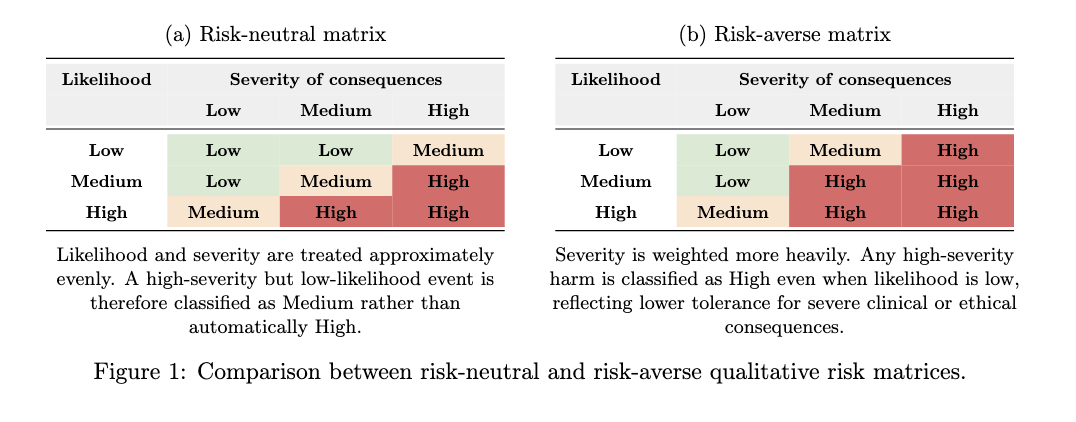
\includegraphics[width=\textwidth]{figures/risk_matrices.png}
    \caption{Qualitative likelihood-vs-severity matrices used in the risk assessment. The risk-neutral matrix (a) is used for commercial and operational risks; the risk-averse matrix (b) is used for clinical, safety and data-governance risks where severity is weighted more heavily.}
    \label{fig:risk-matrices}
\end{figure}

\subsection{Risk Assessment}

The principal risks identified in the report are recorded in \Cref{tab:risk-register} with their source or design limitation, the existing design or procedural control, and the residual limitation that must be verified during Phase 1.

\begin{table}[htbp]
    \centering
    \caption{Qualitative risk register for NeuroScreen.}
    \label{tab:risk-register}
    \footnotesize
    \begin{tabular}{p{2.6cm}p{3.6cm}cp{4cm}p{3.4cm}}
        \toprule
        \textbf{Risk} & \textbf{Source / design limitation} & \textbf{Initial} & \textbf{Mitigation / control} & \textbf{Residual limitation} \\
        \midrule
        \textbf{False negative / false reassurance} \emph{(Clinical)}
            & A ``low risk of mTBI'' output after a genuine mTBI could lead to injured athletes missing treatment.
            & High
            & NeuroScreen must use conservative thresholds, confidence scores and explicit warning statements.
            & NeuroScreen cannot rule out concussion or provide return-to-play clearance. \\
        \midrule
        \textbf{False positive / unnecessary referral} \emph{(Clinical)}
            & Conservative thresholds may incorrectly flag a non-concussed user as requiring further assessment.
            & Medium
            & Present abnormal outputs as ``further assessment recommended'' rather than as a diagnosis.
            & Some unnecessary referrals are acceptable in screening tools but may reduce trust or adoption if frequent. \\
        \midrule
        \textbf{Poor signal quality and image artefacts} \emph{(Technical)}
            & Poor fit, eyelash occlusion, glare, blur, low pupil--iris contrast, optical misalignment or ambient-light contamination may corrupt pupil and gaze measurements.
            & High
            & Use enclosed optics, fixed headset geometry, controlled NIR illumination, image-quality checks, signal-quality flag, confidence score and repeat-test logic.
            & Some users or conditions may produce no valid result; failure-to-test must be treated as safer than false reassurance. \\
        \midrule
        \textbf{Motion artefact and poor fit} \emph{(Operational)}
            & Pitch-side users may move during testing due to anxiety, instability, poor headset fit or recent injury, contaminating PLR, vergence or smooth-pursuit features.
            & High
            & IMU-based motion gating; reject or abort trials when motion exceeds threshold during critical windows; provide repeat-test prompts.
            & Motion rejection protects evidence quality but may reduce completion rate in real field use. \\
        \midrule
        \textbf{Physical user-safety failure} \emph{(Safety)}
            & Near-eye IR illumination, high display brightness, battery faults, overheating or electrical faults could expose the user to harm.
            & High
            & Controlled through the electronics safety architecture already specified: fixed illumination limits, calibrated brightness ceilings, watchdog/timeout behaviour, battery protection, fuel-gauge shutdown and conservative thermal design.
            & Controls are specified at design level but require verified bench and safety testing before Phase 1 human data collection. \\
        \midrule
        \textbf{Timing and synchronisation uncertainty} \emph{(Technical)}
            & PLR latency, pursuit phase lag and vergence timing depend on accurate stimulus and frame timing; the prototype does not yet use medical-grade hardware synchronisation.
            & Medium
            & High-frame-rate capture, timestamp logging, stimulus dwell periods, transition-frame exclusion, and validation against known timing events.
            & Timing uncertainty may bias extracted biomarkers until validated on the final integrated hardware. \\
        \midrule
        \textbf{ML, biomarker and population-validation gap} \emph{(Evidence)}
            & Model performance may not generalise across age, medication, fatigue, eye colour, iris pigmentation, prior TBI, visual history, or real pitch-side conditions.
            & High
            & Conduct governed Phase 1 dataset collection; lock model versions during validation; perform subgroup analysis; compare outputs against clinical assessment; maintain conservative claims.
            & Until clinical validation is complete, NeuroScreen can claim only decision support, not diagnostic accuracy. \\
        \midrule
        \textbf{Supply-chain and manufacturing variability} \emph{(Commercial)}
            & Measurement quality depends on camera selection, beamsplitter performance, optical alignment, display brightness, LED symmetry, calibration consistency and availability of strategic components.
            & Medium
            & Retain optical alignment, calibration, final integration and end-of-line testing in-house; use incoming inspection and second-source critical components where possible.
            & Scaling production may introduce device-to-device variability unless calibration and quality controls mature with volume. \\
        \bottomrule
    \end{tabular}
\end{table}


\section{Quality, Ethics and Sustainability}
\label{sec:ent-ethics}

\subsection{Quality Control System}

The EU conformity assessment in \Cref{sec:ent-regulatory-eu} requires a quality management system aligned with ISO~13485~\cite{iso13485}. It would, however, be unrealistic to propose full commercial quality management within the scope of the 3YP. A more appropriate strategy is a progressive quality-maturity guideline whose obligations rise with the phase of development.

\textbf{Phase 1.} This stage relies heavily on documentation of product iteration covering hardware revision, software version and operator notes. During the data-collection clinical trials, each test session must be traceable to a device identifier, protocol version, stimulus log, software build, preprocessing pipeline, model version and data-processing workflow, ensuring its defensibility with the HRA under the NHS approval pathway in \Cref{sec:ent-regulatory-uk}.

\textbf{Phase 2.} This stage assumes evidence integrity and moves to production-scale repeatability, which requires an ISO~13485-aligned QMS in which design requirements, risk controls, verification tests, supplier records, software releases and complaint feedback are formally linked~\cite{iso13485}. For this device, the highest-priority controls are optical alignment, camera focus, LED brightness, display luminance, IMU function, signal-quality thresholds, model versioning and result wording. Each unit released into Phase~2 pilots should pass an end-of-line test covering frame rate, binocular alignment, illumination symmetry, battery telemetry, thermal behaviour, Bluetooth result transmission, Wi-Fi upload and repeatability on a calibration target. Software and ML updates should move to a controlled release for each pilot period, with any change triggering regression testing and documented review. Pilot feedback, failed tests, discomfort, poor fit, confusing UI interactions and complaints should feed into a corrective-and-preventive-action (CAPA) process.

\subsection{Ethical Considerations}

\textbf{Inclusivity.} Oculomotor measurements vary with age, medication, fatigue, eye colour, iris contrast, prior TBI, visual impairment, and neurological or ophthalmological history~\cite{ortega2022medicalhistory,bergamini1998iriscolour}. The system must therefore be validated across the populations it claims to serve, as set out by Alderman et al.~\cite{alderman2024aitransparency}. For NeuroScreen, the intended user profile is restricted to 12--18 year-olds across a representative range of eye characteristics and medical and neurological history reflected in the dataset collected in Phase 1.

\textbf{Algorithmic transparency.} A non-expert operator does not need to inspect the model weights, but they do need to understand why a test was accepted, rejected or flagged based on signal-quality, motion and confidence indicators. This is sufficient transparency for the user to understand the limits of the result and when further medical assessment is required~\cite{alderman2024aitransparency,who_aiethics2021}.

\textbf{Pricing.} For a health-related product, pricing is not only a revenue model but also determines whether a device remains accessible at the point of need~\cite{who_pricing}. The commercial plan in \Cref{chapter:ent-business} deliberately does not gate emergency screening behind a recurring consumer subscription, instead relying on a one-off hardware sale with an optional institutional subscription for additional administrative features. This is ethically stronger than charging parents continuously for the right to use a device that may only be needed unpredictably after injury.

\subsection{Lifecycle, Environmental Impact and Sustainability}

A full lifecycle assessment (LCA) sits alongside the EU MDR technical file, risk management, post-market surveillance and CE-marking pathway. The appropriate framework for that future assessment is ISO~14040/14044, which defines LCA in terms of goal and scope, life-cycle inventory, impact assessment and interpretation~\cite{iso14040}.

The relevant product lifecycle has five stages: component sourcing, assembly and calibration, use, maintenance and end-of-life. Components such as electrical and electronic assemblies, camera modules, the display, PCB assemblies, optical components, the LiPo battery, enclosure materials and straps must therefore be selected with the EU RoHS restrictions on hazardous substances, REACH chemical obligations, and EU battery requirements in mind~\cite{eu_rohs,eu_reach,eu_batteries}.

Assembly and initial calibration are enforced by end-of-line testing with periodic functional checks for battery ageing, cleaning, storage effects and software updates, as set out in the quality plan above. Maintenance is supported by replaceable straps, facial interface, battery, camera modules, illumination board and (potentially) the display, with any replacement triggering device recalibration.

End-of-life can be distinguished between reusable, refurbishable and waste components. Returned Phase~1 or Phase~2 devices may still be useful for training or software testing even if unsuitable for commercial redeployment. Batteries require controlled disposal under the EU battery regulation~\cite{eu_batteries}; PCBs, cameras and display electronics enter WEEE-compliant waste streams~\cite{eu_weee}; and packaging must comply with the EU packaging-waste regulation~\cite{eu_packaging}.

The main environmental impacts are concentrated in electronics manufacture, battery replacement and disposal, and cloud data transfer. The sustainability strategy is therefore to adopt design decisions that reduce future impact: modular repair, replaceable batteries, reusable or refurbishable returned units, and compliant disposal of electronic waste. This becomes especially important in Phase~3, where wider amateur-sport distribution increases the number of devices outside direct company control.


\appendix

\include{appendix_1}
\chapter{Supporting analyses}
\label{appendix:supporting-analyses}

\section{Prior-art search methodology for \S6.3.1}
\label{appendix:prior-art-search}

This appendix documents the prior-art scan that informs the patentability analysis in \Cref{sec:ent-patentability}. It is presented as a methodological appendix, not as a substitute for a formal freedom-to-operate (FTO) opinion by patent counsel.

\subsection*{Calibration disclaimer}

This is an academic prior-art scan, not a freedom-to-operate opinion or legal advice. The search corpus is publicly indexed Google Patents, Espacenet and USPTO Public Search; no fee-based databases (Derwent, PatBase, IFI Claims, IPlytics) were consulted. All conclusions are framed as \emph{appears}, \emph{based on this scan}, \emph{likely}. An issued patent identified below is not necessarily blocking: a real FTO must read individual claims. Conversely, a journal or press disclosure is prior art for novelty under \S102 / Art.~54 EPC but is not an infringement risk.

\subsection*{Search engines}

\begin{itemize}
    \item Google Patents (\texttt{patents.google.com}) --- full-text plus citation graph; both granted and published-application records.
    \item Espacenet (EPO/WIPO/UKIPO full-text), cross-checked via Google Patents.
    \item USPTO Patent Public Search --- confirmation of US grant numbers.
    \item Justia Patents --- assignee and classification index.
    \item Secondary press/aggregator sources (Patently Apple, nweon Patent, EurekAlert, GlobeNewswire) for assignee--product linkage.
\end{itemize}

\subsection*{Search strings (representative)}

\begin{itemize}
    \item \texttt{"beamsplitter" eye tracking pupillometry patent}
    \item \texttt{"dichroic" "850 nm" eye tracking head-mounted display patent}
    \item \texttt{"hot mirror" eye tracking patent VR HMD pupil tracking}
    \item \texttt{"longpass dichroic" beamsplitter eye imaging patent pupil 750 nm}
    \item \texttt{"binocular vergence" pupillometry concussion patent headset}
    \item \texttt{"pupillary light reflex" patent headset goggles concussion screening}
    \item Assignee queries: NeurOptics, Apple Inc., Magic Leap, Oculus/Meta/Facebook, Tobii, SyncThink/Neurosync, Oculogica, Neuro Kinetics/Neurolign/Spryson, 3M, Elbit Systems, Novutz LLC, Indiana University Research and Technology Corp, Purdue Research Foundation, University of Miami.
\end{itemize}

\subsection*{Classification codes used (CPC / IPC)}

\begin{itemize}
    \item A61B 3/113 --- Objective instruments for examining eye movement.
    \item A61B 3/14 --- Arrangements specially adapted for taking photographs of the eye.
    \item A61B 5/0059 --- Detecting/measuring for diagnostic purposes by tracking eye-movement pattern.
    \item G02B 27/14 --- Beam splitting or combining systems based on path interference.
    \item G02B 27/01 --- Head-up displays / head-mounted displays.
    \item G06V 40/19 --- Sensor that detects gaze direction.
\end{itemize}

\subsection*{Date range}

Searches were not date-bounded. Hits range from 1992 (US5,345,281A) to 2025 grants (e.g.\ US12,311,584). The planned priority filing window is 2026--2027; any patent or publication pre-dating priority is potential anticipating prior art.

\subsection*{Coverage limits}

No fee-based prior-art database (Derwent, PatBase, IFI Claims, IPlytics) was consulted. All queries are keyword-based; no structured semantic search. Non-patent literature (NPL) was scanned only opportunistically through patent-database back-references and through targeted academic searches for BrainEye, FOVE-VR, and concussion-screening publications. Foreign-language patents (CN, JP, KR) were reachable via Google Patents machine translation but were not exhaustively scanned. A real FTO would require reading independent claims of each issued patent element-by-element against the proposed device's draft claim set.

\subsection*{Most-relevant references identified}

The twelve most novelty-impacting records identified are catalogued, with assignee, filing/priority date, relevance, and novelty-impact assessment, in the internal audit working file (not reproduced in this report for length reasons; available on request). The five highest-impact entries are: \citet{taboada1994}, \citet{neuropticspatent2017}, \citet{neurokineticshmd2017}, \citet{krueger2014ocular}, and \citet{syncthinkpatent2015}; each is cited in \Cref{sec:ent-patentability} above.


\backmatter
\listofreferences[unsrtnat]

\end{document}
